%%%%%%%%%%%%%%%%%%%%%%%%%%%%%%%%%%%%%%%%%
% Masters/Doctoral Thesis 
% LaTeX Template
% Version 2.5 (27/8/17)
%
% This template was downloaded from:
% http://www.LaTeXTemplates.com
%
% Version 2.x major modifications by:
% Vel (vel@latextemplates.com)
%
% This template is based on a template by:
% Steve Gunn (http://users.ecs.soton.ac.uk/srg/softwaretools/document/templates/)
% Sunil Patel (http://www.sunilpatel.co.uk/thesis-template/)
%
% Template license:
% CC BY-NC-SA 3.0 (http://creativecommons.org/licenses/by-nc-sa/3.0/)
%
%%%%%%%%%%%%%%%%%%%%%%%%%%%%%%%%%%%%%%%%%

%----------------------------------------------------------------------------------------
%	PACKAGES AND OTHER DOCUMENT CONFIGURATIONS
%----------------------------------------------------------------------------------------

\documentclass[
11pt, % The default document font size, options: 10pt, 11pt, 12pt
oneside, % Two side (alternating margins) for binding by default, uncomment to switch to one side
english, % ngerman for German
onehalfspacing, % Single line spacing, alternatives: onehalfspacing or doublespacing
%draft, % Uncomment to enable draft mode (no pictures, no links, overfull hboxes indicated)
%nolistspacing, % If the document is onehalfspacing or doublespacing, uncomment this to set spacing in lists to single
%liststotoc, % Uncomment to add the list of figures/tables/etc to the table of contents
%toctotoc, % Uncomment to add the main table of contents to the table of contents
%parskip, % Uncomment to add space between paragraphs
%nohyperref, % Uncomment to not load the hyperref package
headsepline, % Uncomment to get a line under the header
%chapterinoneline, % Uncomment to place the chapter title next to the number on one line
%consistentlayout, % Uncomment to change the layout of the declaration, abstract and acknowledgements pages to match the default layout
]{MastersDoctoralThesis} % The class file specifying the document structure

\usepackage[utf8]{inputenc} % Required for inputting international characters
\usepackage[T1]{fontenc} % Output font encoding for international characters
\usepackage{pdfpages}
\usepackage{mathpazo} % Use the Palatino font by default
\usepackage{todonotes}
\usepackage{menukeys}
%\usepackage{natbib}

% Uncomment the next two lines to use the biber command.
\usepackage[style=numeric]{biblatex} % Use the bibtex backend with the authoryear citation style (which resembles APA)
\addbibresource{reference_library.bib} % The filename of the bibliography

\usepackage[autostyle=true]{csquotes} % Required to generate language-dependent quotes in the bibliography

%----------------------------------------------------------------------------------------
%	MARGIN SETTINGS
%----------------------------------------------------------------------------------------

\geometry{
	paper=a4paper, % Change to letterpaper for US letter
	inner=2.5cm, % Inner margin
	outer=3.8cm, % Outer margin
	bindingoffset=.5cm, % Binding offset
	top=1.5cm, % Top margin
	bottom=1.5cm, % Bottom margin
	%showframe, % Uncomment to show how the type block is set on the page
}

%----------------------------------------------------------------------------------------
%	THESIS INFORMATION
%----------------------------------------------------------------------------------------

\thesistitle{8-bit Innovation: The challenges facing community based and open-source retro-computing projects} % Your thesis title, this is used in the title and abstract, print it elsewhere with \ttitle
\supervisor{Dr. Paul \textsc{Gardner-Stephen}} % Your supervisor's name, this is used in the title page, print it elsewhere with \supname
\examiner{} % Your examiner's name, this is not currently used anywhere in the template, print it elsewhere with \examname
\degree{Bachelor of Engineering (Software) (Honours)} % Your degree name, this is used in the title page and abstract, print it elsewhere with \degreename
\author{Tom \textsc{Aylen}} % Your name, this is used in the title page and abstract, print it elsewhere with \authorname
\addresses{} % Your address, this is not currently used anywhere in the template, print it elsewhere with \addressname

\subject{Software Engineering} % Your subject area, this is not currently used anywhere in the template, print it elsewhere with \subjectname
\keywords{} % Keywords for your thesis, this is not currently used anywhere in the template, print it elsewhere with \keywordnames
\university{\href{http://www.flinders.edu.au}{Flinders University}} % Your university's name and URL, this is used in the title page and abstract, print it elsewhere with \univname
\department{\href{https://www.flinders.edu.au/college-science-engineering}{College of Science and Engineering}} % Your department's name and URL, this is used in the title page and abstract, print it elsewhere with \deptname
\group{\href{http://researchgroup.university.com}{Research Group Name}} % Your research group's name and URL, this is used in the title page, print it elsewhere with \groupname
\faculty{\href{http://www.flinders.edu.au/college-science-engineering}{Faculty of Science and Engineering}} % Your faculty's name and URL, this is used in the title page and abstract, print it elsewhere with \facname

\AtBeginDocument{
\hypersetup{pdftitle=\ttitle} % Set the PDF's title to your title
\hypersetup{pdfauthor=\authorname} % Set the PDF's author to your name
\hypersetup{pdfkeywords=\keywordnames} % Set the PDF's keywords to your keywords
}

\begin{document}

\frontmatter % Use roman page numbering style (i, ii, iii, iv...) for the pre-content pages

\pagestyle{plain} % Default to the plain heading style until the thesis style is called for the body content

%----------------------------------------------------------------------------------------
%	TITLE PAGE
%----------------------------------------------------------------------------------------

\begin{titlepage}
\begin{center}

\vspace*{.06\textheight}
{\scshape\LARGE \univname\par}\vspace{1.5cm} % University name
\textsc{\Large Honours Thesis}\\[0.5cm] % Thesis type

\HRule \\[0.4cm] % Horizontal line
{\huge \bfseries \ttitle\par}\vspace{0.4cm} % Thesis title
\HRule \\[1.5cm] % Horizontal line
 
\begin{minipage}[t]{0.4\textwidth}
\begin{flushleft} \large
\emph{Author: }\\
\authorname
\end{flushleft}
\end{minipage}
\begin{minipage}[t]{0.4\textwidth}
\begin{flushright} \large
\emph{Supervisor:} \\
\supname
\end{flushright}
\end{minipage}\\[3cm]
 
\vfill

\large \textit{Submitted to the \\\deptname \\ in the \\\facname \\
in partial fulfilment of the requirements for the degree of \\\degreename\\ 
at Flinders University - Adelaide, Australia} \\[3cm]
%University requirement text

 
\vfill

{\large \today}\\[4cm] % Date
%\includegraphics{Logo} % University/department logo - uncomment to place it
 
\vfill
\end{center}
\end{titlepage}

%----------------------------------------------------------------------------------------
%	DECLARATION PAGE
%----------------------------------------------------------------------------------------

\begin{declaration}
\addchaptertocentry{\authorshipname} % Add the declaration to the table of contents
\noindent I certify that this work does not incorporate without acknowledgement any material previously submitted for a degree or diploma in any university; and that to the best of my knowledge and belief it does not contain any material previously published or written by another person except where due reference is made in the text.\\
 
\noindent Signed:\\
\rule[0.5em]{25em}{0.5pt} % This prints a line for the signature
 
\noindent Date:\\
\rule[0.5em]{25em}{0.5pt} % This prints a line to write the date
\end{declaration}

\cleardoublepage

%%----------------------------------------------------------------------------------------
%%	QUOTATION PAGE
%%----------------------------------------------------------------------------------------
%
%\vspace*{0.2\textheight}
%
%\noindent\enquote{\itshape Thanks to my solid academic training, today I can write hundreds of words on virtually any topic without possessing a shred of information, which is how I got a good job in journalism.}\bigbreak
%
%\hfill Dave Barry

%----------------------------------------------------------------------------------------
%	ABSTRACT PAGE
%----------------------------------------------------------------------------------------

\begin{abstract}
  \addchaptertocentry{\abstractname} % Add the abstract to the table of contents
  The children who grew up through the home computer revolution of the 1980s are now
  established in life, and frequently willing to invest time and money in projects and products that have nostalgic
  value for them.  This includes retro-computing projects that re-create the iconic
  home computers of the 1980s and early 1990s.
  There have been a number of community and commercially driven retro-computing projects,
  such as the Spectrum Next, Spectrum Vega, the C64mini, the C64DTV, the Ultimate64 among
  many others. The scope and ambition of these projects varies, as has their success.
  Some, like the C64DTV were commercial successes, while others, such as the Spectrum
  Vega are suffering long drawn out deaths due to a variety of problems or misadventures.
  The purpose of this research is to examine a number of these as case-studies, and to
  learn from them, so that other such projects can have an increased likelihood of success,
  and the participants can avoid some of the more unpleasant misadventures that have arisen,
  especially those involving hostile lawyers.
  This thesis acts to document the steps and stages of productisation and market release for
  such projects, and then applies these learnings directly to the MEGA65 retro-computing
  project at Flinders University, to accelerate its approach to market, and to help it avoid
  the pitfalls of past failures.  The learnings presented in this thesis are designed to be
  of use to any retro-computing project, and it is our hope that it will enable other
  projects to also have greater success, and less pain in the process. 
  \citep{CNN_c64_recall}
  

 
 
\end{abstract}

%----------------------------------------------------------------------------------------
%	ACKNOWLEDGEMENTS
%----------------------------------------------------------------------------------------

\begin{acknowledgements}
\addchaptertocentry{\acknowledgementname} % Add the acknowledgements to the table of contents
Wonderful positive statements go here.
\end{acknowledgements}

%----------------------------------------------------------------------------------------
%	LIST OF CONTENTS/FIGURES/TABLES PAGES
%----------------------------------------------------------------------------------------

\tableofcontents % Prints the main table of contents

\listoffigures % Prints the list of figures

\listoftables % Prints the list of tables

%----------------------------------------------------------------------------------------
%	ABBREVIATIONS
%----------------------------------------------------------------------------------------

\begin{abbreviations}{ll} % Include a list of abbreviations (a table of two columns)

\textbf{CPU} & \textbf{C}omputer \textbf{P}rocessing \textbf{U}nit\\
\textbf{PCB} & \textbf{P}rinted \textbf{C}ircuit \textbf{B}oard\\
\textbf{IC} & \textbf{I}ntegrated \textbf{C}ircuit\\

\end{abbreviations}

%----------------------------------------------------------------------------------------
%	DEDICATION
%----------------------------------------------------------------------------------------

\dedicatory{For/Dedicated to/To my\ldots} 

%----------------------------------------------------------------------------------------
%	THESIS CONTENT - CHAPTERS
%----------------------------------------------------------------------------------------

\mainmatter % Begin numeric (1,2,3...) page numbering

\pagestyle{thesis} % Return the page headers back to the "thesis" style

% Include the chapters of the thesis as separate files from the Chapters folder
% Uncomment the lines as you write the chapters

%% Chapter 1 - Introduction
\chapter{Introduction} % Main chapter title
\label{Chapter1} % For referencing the chapter elsewhere, use \ref{Chapter1} 
%Copied from Thesis Topic Manual
%Introduction
%The introduction should provide the following:
% background to the topic;
% brief review of current knowledge (this is not the literature review – it’s only a high level overview);
% state hypotheses;
% indicate gaps in knowledge, state aims of the thesis and how it fits into the gap;
% an outline of the following chapters.

% The introduction should follow the recommended structure:
% state the general background of the thesis topic and give some background
% provide an overview of the literature related to the thesis topic
% define the terms and scope of the thesis
% outline the current situation
% evaluate the advantages/ disadvantages of existing solutions and identify the knowledge gap
% identify the importance of the proposed research
% state the research problem/ questions
% state the research aims and/or research objectives
% state the hypotheses
% outline the experiment methodology
% outline the structure of the thesis
%----------------------------------------------------------------------------------------
%----------------------------------------------------------------------------------------
\section{Background}
A retro-computing project is a computing project that is in some way inspired or derived from a home computer the was released between about 1975 and 1990 \cite{magerkurth2004augmenting,suominen2015return}. This period is referred to as the early home computer era and it was the first time computers where specifically marketed for personal use within the home. This lead to many people having their first interaction with a computer during this period. Many people whom lived through this period have strong memories of the products they used, such as the Commodore 64, the ZX Spectrum and the BBC Micro. 

For various reasons, many people have tried, with varying amounts of success, to revive certain computer systems from the period, either by emulating the system in software on a more powerful computer, or by rebuilding the physical circuitry. Some retro-computing projects have been inspired by the home computers of the period being simpler and having less abstraction between the user and the mechanics of the computer. The MEGA65 is a retro-computing project which is currently under development and which aims to innovate the never-released Commodore 65 \cite{mega65}. 


\section{Scope of thesis}
This thesis aims to provide a body of knowledge on the process, as well as the challenges and risks associated with retro-computing projects when trying to bring new products to market. 

The general product development process has been widely explored from many different angles by various authors over time, e.g., \cite{veryzer1998discontinuous,imai1984managing,schilling1998managing,morgan2006toyota,zahay2018managerial,sommer2015improved,stark2015product,rajagopalan2017exploring,chahin2016practical}.  The general product development concept and process is beyond the scope of this thesis, which instead focuses on the issues particular to retro-computing projects.

\section{Current situation and how it can be improved}
Many retro-computing projects have brought products to the market, with varying amounts of success. The C64 Mini is a Commodore 64-inspired game console which is available for purchase from retail outlets within Australia and other countries. It received satisfactory reviews and can be considered a successful project by many metrics. Comparatively, the Vega Plus, a hand-held game console inspired by the Spectrum ZX, was an abject failure in regard to project outcomes for stakeholders. The widely varying processes and methods employed by differing projects suggests the outcomes may be more consistent and improved if a more rigorous process was followed. 

There is currently no body of knowledge specific to retro-computer projects and the productization process. If a body of knowledge could be formed it should allow future projects to achieve a more consistent outcome. This thesis aims to be the start point for that body of knowledge and it is hoped further research will follow. Part of this thesis is to highlight the common challenges and risks that retro-computing projects are likely to be exposed to, which should allow retro-computing projects to be evaluated against aforementioned risks. With a risk evaluation undertaken and the high risk areas identified, the retro-computing projects should be able to determine and enact strategies to reduce their risk exposure, this should then have the effect of improving the outcomes of the project.

\section{Research questions}
The questions this thesis aims to answer are:
\begin{enumerate}
\item What does the retro-computing project productization process look like?
\item What risk and challenges are associated with a retro computing revival project?
\item What is the MEGA65 project? 
\item How exposed to risks was the MEGA65 project in July 2018?
\item What can be done to reduce the MEGA65 project's risks?
\item Did the MEGA65 project reduce its risk after 10 months?
\end{enumerate}


\section{Hypothesis}
It is hypothesised that the body of knowledge created as part of this thesis, which includes a definition of the process to productization of a retro-computing project as well as its associated risks and challenges, will allow future retro-computing projects to achieve more desirable outcomes more consistently.


\section{Methodology}
The method which was followed to create the body of knowledge and answer the research questions is described here. 

First an in-depth case study was conducted into several retro-computing projects. Because there is a lack of peer-reviewed sources for this information, a majority of this information was sourced from websites and other publications. From these case studies a process was distilled and recorded. The challenges that beset each project were recorded and then categorised into a list of risks. 

As a way to assess the utility of the list of identified risks, a retro-computing project is evaluated twice over a 10 month period against the identified risks. This project, called MEGA65, is a retro-computing project which is currently in development, making it an ideal candidate to evaluate. After the first evaluation the MEGA65 project is provided with advice and strategies on how to reduce their risk exposure in the areas identified as high risk in the evaluation. After ten months the MEGA65 project is evaluated again and the results compared to determine if the MEGA65 project's risk expose has changed. 

To evaluate the MEGA65 project effectively, it first needed to be understood, this process involved researching the state of the MEGA65 project in July 2018 as well as researching the intended products to be released by the MEGA65 project. The products MEGA65 intends to release are captured with a use case study which looks at ways the users will interact with the products. To understand the state of the MEGA65 and its development, most of the information was conveyed via conversations with the MEGA65 team members. This is due to the nature of the development process not allowing time for documentation to be created with all of the relevant details. 

\section{Contributions}
The contributions this thesis makes to retro-computing projects is categorised as follows:
\begin{enumerate}
\item Creates a body of knowledge exploring the retro-computing project productization process.
\item Creates a body of knowledge discussing the risks and challenges associated with retro-computing projects.
\item A risk evaluation of a specific retro-computing project, the MEGA65.
\item Practical, actionable recommendations to reduce the MEGA65 project's risk exposure.
\item Evidence of the benefit of those recommendations, gathered through a follow-up risk evaluation of the MEGA65 several months after providing the recommendations.
\end{enumerate}

\section{Structure of thesis}
This thesis is structured as follows. After this introductory chapter there is a literature review in chapter \ref{Chapter2}. 

Chapter \ref{Chapter3} consists of case studies into several retro-computer projects with a focus on the process they followed and the challenges they faced in releasing a new product. After the case studies there is a discussion and synthesis of the productization process illuminated from the case studies. The challenges extracted from the case studies are then categorised into risks and these risks discussed and rated in terms of potential damage to retro-computing projects. 

Chapter \ref{Chapter4} is dedicated to explaining the MEGA65 project, its intended products and their state of development as of July 2018. This explanation takes the form of a description of the various aspects of the MEGA65 project, including the project's team characteristics, funding model and the products they are creating. Following the description of the MEGA65, there is a use case study conducted into the MEGA65 project's intended products, the MEGAphone and the desktop form-factor of the MEGA65, also called the MEGA65. 

A risk evaluation of the MEGA65 project in July 2018, provides the bulk of chapter \ref{Chapter5}. Following the evaluation, the identified high-risk areas are discussed and advice is provided to the MEGA65 project on how to reduce their risk exposure. 

Finally, chapter \ref{Chapter6} provides a second risk evaluation, taken 10 months after the first. The two risk evaluations are then compared and the changes in risk exposure are highlighted. A discussion of the results of the comparison and a conclusion follows, which ends the body of the thesis.

%%Chapter 2 - Literature Review

\chapter{Literature Review} % Main chapter title
\label{Chapter2} % For referencing the chapter elsewhere, use \ref{Chapter2} 

%----------------------------------------------------------------------------------------
%----------------------------------------------------------------------------------------
\section{Early home computer era} \label{sec: Early home computer era}
 
The mid-1970s to late-1980s was an interesting period in the history of computers. It marked the first time computers were designed and marketed for personal use in the home; the early home computer era. The term \textit{home computer} is ambiguous and not defined by any standard. In this thesis it is taken to be synonymous with a microcomputer or a personal computer (PC) from the era. A PC is classified in the \textit{Proceedings of the IEEE} from 1984 by Gupta, A. and Toong, H. as a computer that fulfils all of the following characteristics 
\cite{RN24}: 

\begin{enumerate}
\item The computer cost less than \$5000 USD at the time of sale.
\item The computing power is provided by a microprocessor from the era. 
\item The computer is sold through mass-marketing channels. 
\item The computer can run a variety of programs for different fields such as industry, business, education and at home; it is a general purpose computer, not designed for a single purpose or a single type of user.
\item The computer can handle at least one high-level language such as BASIC, FORTRAN, or COBOL.
\end{enumerate}

Since the discovery of semiconductors in the 1940s, there have been continuous efforts and advances in making electronic devices smaller, more powerful and cheaper. 1958 saw the first working Integrated Circuit (IC, also called a microchip or chip), continuing this trend 
\cite{RN36}. By 1965, Gordon E. Moore was talking about the observation that ICs are being manufactured with an increasing amount of components, which came to be popularly known as "Moore's Law" 
\cite{RN33}. In 1971, Intel developed the first microprocessor; the 4-bit 4004 on a single IC 
\cite{RN37}, shown in figure \ref{Intel4004}. A microprocessor is an entire CPU within an IC or a few ICs. The following year, Intel released the more powerful 8-bit 8008 microprocessor. Then in 1974 an even more powerful microprocessor was released by Intel, the 8080. 
\cite{RN38}. 

\begin{figure} \begin{center}
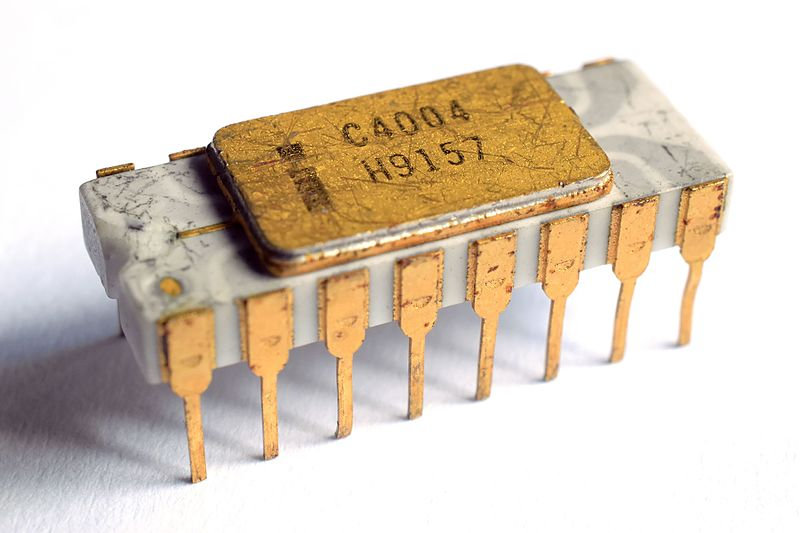
\includegraphics[width=.3\linewidth]{pics/intel_4004} 
\end{center} 
\caption{Intel 4004 microprocessor, an entire CPU on a single chip; the first microprocessor. Released in 1971.\\ \textit{\small{Picture courtesy of Thomas Nguyen}}}
\label{Intel4004}
\end{figure} 

It seems a tipping point had now been reached, the manufacturing cost of computers was low enough, their size was small enough and their performance was high enough that some manufacturers decided to start designing and marketing them to personal users. In 1974, MITS released what can be considered the first market-successful home computer 
\cite{RN41}, the Altair 8800, which used an 8080 microprocessor and is shown in figure \ref{Altair8800}.

\begin{figure} \begin{center}
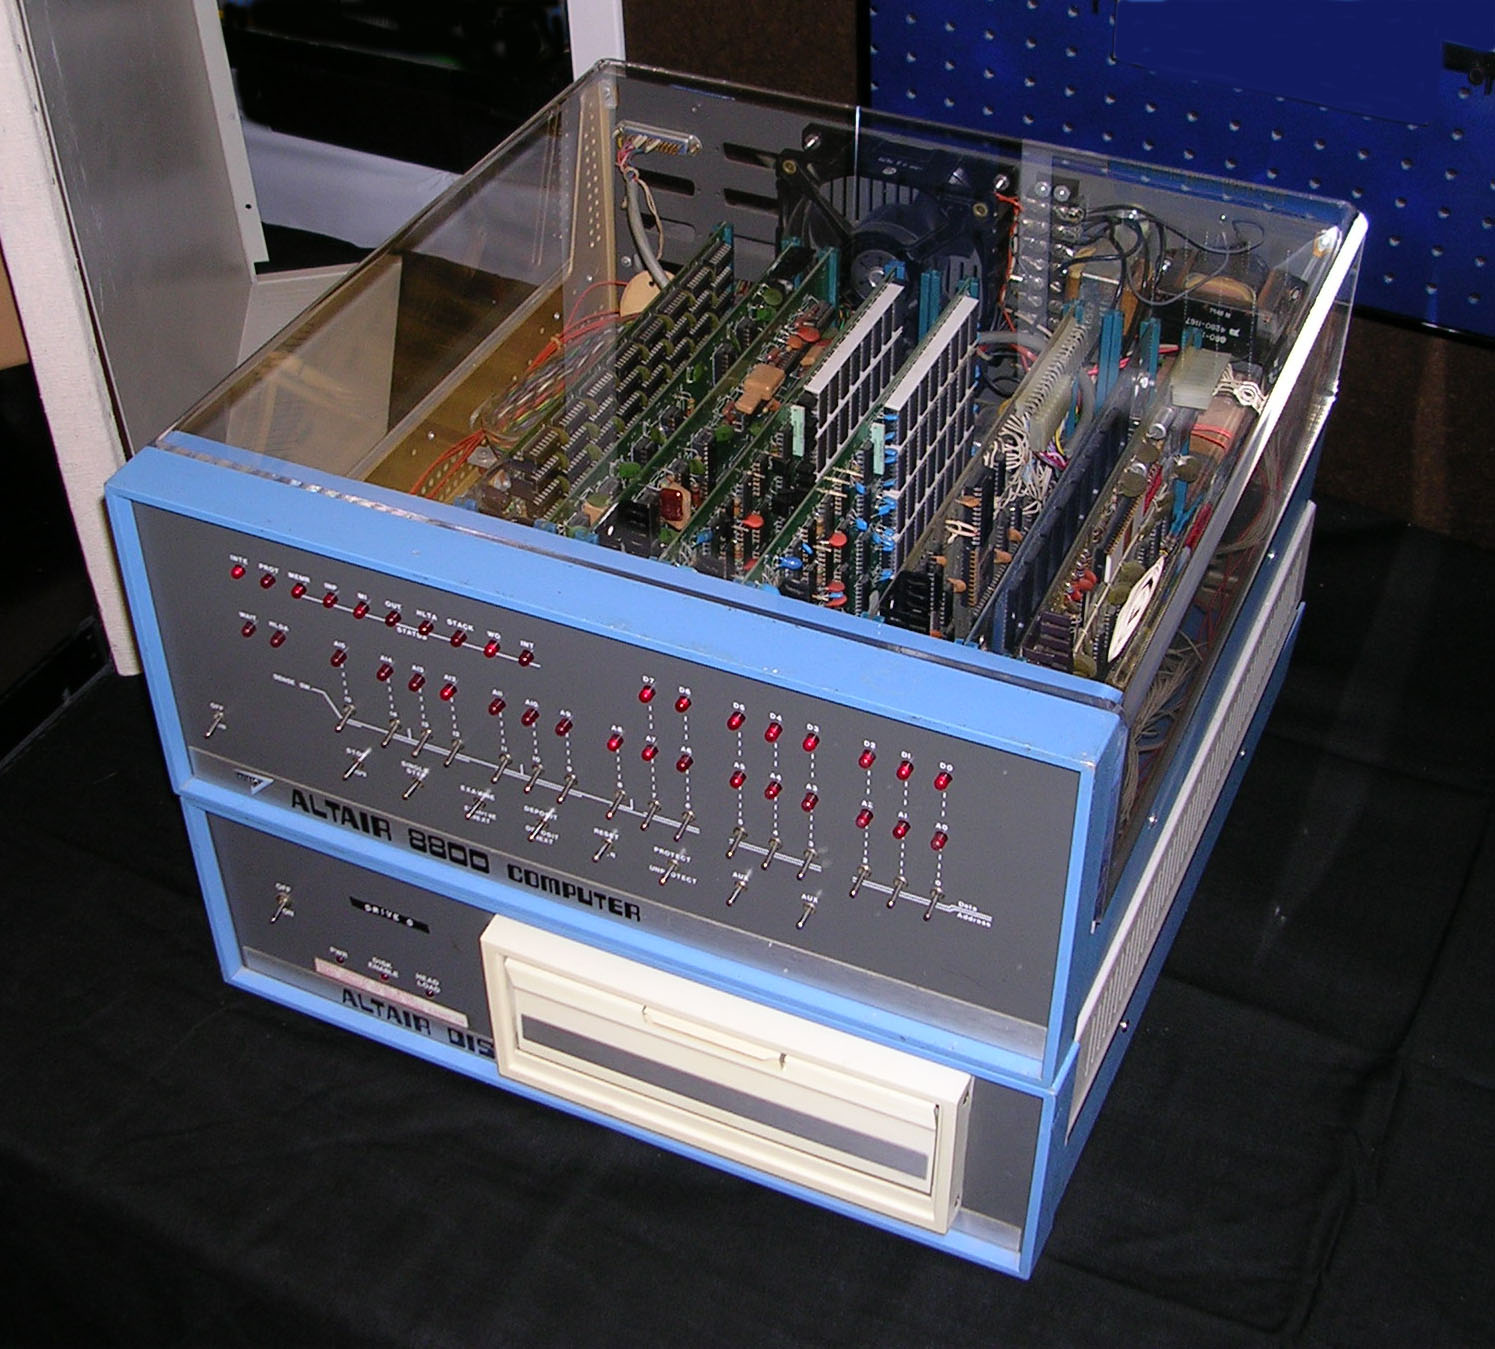
\includegraphics[width=.3\linewidth]{pics/altair_8800_computer} 
\end{center} 
\caption{MITS Altair 8800 home computer, the first market successful home computer. It used an 8-bit 8080 microprocessor and was released in 1974.\\ \textit{\small{Picture courtesy of Michael Holley}}}
\label{Altair8800}
\end{figure}

Over the next 15 or so years, a flurry of new companies sprung up offering a multitude of personal computers 
\cite{RN27}. In the same period new microprocessors where developed, further increasing their performance and new processes where developed that reduced their cost to manufacture. The most notably of these new microprocessors is the 8-bit 6502 by MOS Technology, which when released in 1975 was the least expensive microprocessor on the market by a sizeable margin 
\cite{RN40}. A sense of excitement and seemingly an expectation that computers where going to revolutionise society was abound at this time 
\cite{RN34}. Many people were having their first interactions with computers, as the home computer became more wide spread.

These early home computers had a relatively simple interface compared to modern computers. This meant there was far less abstraction between the user and the inner workings of the computer, this may have allowed their users to more readily understand the underlying mechanisms. It also meant that users had to learn at least some rudimentary programming skills to use them. Another way users where exposed to programming was from the possibility to acquire programs by typing them into their own computers out of magazines or from computer shows on TV and thus exposing them to source code. Most of the home computers in this period ran some form of BASIC, which is a family of general-purpose high-level programming languages, all derived from the original BASIC language created at Dartmouth College in 1964
\cite{RN130}. 

There were some people that questioned the usefulness of the early home computers, and with some merit, as there was a lack of software and distribution channels at the beginning of the era
\cite{RN23}. Others had unrealistic expectations of what computers would do for them, including doing tasks such as putting the rubbish out and babysitting. Home computers where mainly used in a four areas: business, science and engineering, education and in the home. Business, science and engineering uses included spreadsheets, word processing, basic graphics, databases and communication to connect to host computer or LANs. In the home the most widely reaching use of home computers was to play games 
\cite{RN24}. These 8-bit home computers were where many people first met and became interested in the potential of computers and computer programming and they helped kick off a revolution.


%----------------------------------------------------------------------------------------
%----------------------------------------------------------------------------------------
\section{Commodore 64, 128, 65}
\subsection{Commodore 64}
The Commodore 64 (C64) was one of the most successful home computers, selling over 17 million units according to Commodore International 
\cite{RN42}, the now defunct manufacturers of the Commodore 64. Earning it a Guinness World Record (formally Guinness Book of Records): 'Most computer sales'
\cite{RN43}.
It was first sold in January, 1982, for \$595 USD at launch 
\cite{RN28}. The computational power came from a 8-bit MOS Technology 6510 microprocessor, a modified version of the 6502 mentioned in section \ref{sec: Early home computer era}. It had 64 kilobytes of RAM, which was the inspiration of its name. The Commodore 64 was a dominant market presence; in a category of influential home computers, the Commodore 64 may well have been the most influential of all. It ran a version of BASIC and there was a huge software library created for it during its lifetime and there's still new software being developed for the C64 to this day.
\cite{RN82}\cite{RN83}\cite{RN84}.

\subsection{Commodore 128}
The Commodore 128 (C128) was Commodore International's evolution of the very successful Commodore 64. Released in January, 1985, It was meant to build on the success of the C64 while still being near 100\% compatible with Commodore 64 software. It was powered by a more powerful 8-bit 8502 microprocessor and had 128 kilobytes of RAM. An innovation was the inclusion of a second microprocessor, an 8-bit Zilog Z80. This second CPU allowed the C128 to run the CP/M operating system as well as the Commodore BASIC environment similar to the C64. Running CP/M allowed the C128 to access the CP/M software library, which was quite extensive. That coupled with the Commodore 64 software library gave the C128 one of the broadest range of software compared to its competitors of the day
\cite{RN32}.

\subsection{Commodore 65}
The Commodore 65 (C65) was in development in 1990-1991, when Commodore Business Machines (subsidiary of Commodore Intentional) went bankrupt in 1994. In the fallout of the collapse, a number of C65 prototypes where sold and are now a rare and valuable collectors item \cite{RN132}. The C65 was planned to be an upgrade of the C64. \textit{Compute! Gazette} reported in an article in 1989 that the C65 had a 16-bit 65816 microprocessor; a 16-bit version of the 6502 
\cite{RN31}. Years later, when the prototypes where sold on the market by liquidators, sources report a modified 65CE02 microprocessor was used instead
\cite{RN30}
\cite{RN78}. The 65CE02 was an 8-bit CPU with a limited ability to use 16-bit instructions. It had 128 kilobytes of RAM, expandable to 1 megabyte. The C65 had a "stunning" 640x400 pixel maximum resolution 
\cite{RN31} powered by a VIC-III graphics chip. It had a C64 compatibility mode, meant to allow near 100\% compatibility with the C64, but the existing prototypes have significant compatibility problems
\cite{RN30}. 

%----------------------------------------------------------------------------------------
%----------------------------------------------------------------------------------------
\section{History of the MEGA65 project}
\label{History of the MEGA65 project}
Started in December 2013 by Dr. Paul Gardner-Stephen 
\cite{RN44}, the MEGA65 project is attempting to innovate the Commodore 65, with near 100\% compatibility with C64 software. Dr. Gardner-Stephen owned a Commodore 65 prototype between 1994-2010, he also owned a Commodore 128 through the same time and when compared, preferred the C65. Dr. Gardner-Stephen also loved to tinker with these computers during the 1990 and 2000s, devising ways of accelerating the C64 CPU as an example. After deciding to sell the C65 prototype to a collector, Dr. Gardner-Stephen always had the idea of recreating the C65, and implementing some of the tricks and ideas he had worked out or heard of over the years. Then, during Dr. Gardner-Stephen's Ph.D studies, he learnt to program in VHDL and it seemed possible to realise this dream using the technology of FPGAs.

This dream was delayed due to technological issues with the FPGA boards of the time not quite being fast enough for Dr. Gardner-Stephen's vision. But by 2013, a sufficiently powerful and affordable board had been released to the market. Dr. Gardner-Stephen chose a Nexys4 development board, used by a lot of teaching institutions and designed with students in mind. This FPGA has many built in peripherals which can be used by the computer as well as its cost to performance ratio makes it ideal. The added benefit of using off-the-shelf FPGA board is that availability should be much greater compared to a PCB created just for MEGA65, which would be limited to small production runs carried out by the MEGA65 team or others using the open-source designs 
\cite{RN45}.

The MEGA65 project is completely open-source with the hardware VHDL/verilog files describing the hardware and operating system software available on a public git repository 
\cite{RN17}. Dr. Gardner-Stephen's stated goals at the inception of the MEGA65 project were as follows \cite{RN45}:

\begin{itemize}[before=\itshape]
\item Better graphics than the Apple IIgs, Atari 800 or Plus/4: 1920x1200 @ 60Hz, 256 colour palette from 4,096 colours (later from 24-bit colour palette once I create an HDMI output) via my VIC-IV video controller.
 \item    Better sprites than the C64.  Plan is for the 8 compatibility sprites, plus perhaps 32 256-colour Enhanced Sprites with hardware scaling and practically unlimited size.  Maximum number of displayable sprites will depend on the resolution of the display and the sprites on a given raster line.
 \item    Faster CPU than the SuperCPU or any available 65C816 CPU (20MHz), and ideally with enough headroom to beat a 20MHz 65C816 running in 16-bit mode.  Currently the 65GS10 runs at 96MHz, but with an effective speed more like 48MHz until I work on some planned IPC improvements, like a 16-bit cache of zero-page to make zero-page indirect instructions take as little as 3 cycles.
 \item    More RAM than a fully expanded Apple IIgs or C65 (~8.125MB).  It will initially have 128KB of chipram like the C65, plus 16MB of slowram, plus "some" ROM.
 \item    Comparable or better sound capability than the Apple IIgs.  Multiple SIDs plus digital audio channels.  Design to be finalised.
 \end{itemize}  

  
After discussions to make sure their goals where aligned, In April 2015, Dr. Gardner-Stephen and the Museum of Electronic Games and Art (MEGA) announced a partnership to make an open-source Commodore 65-like computer 
\cite{RN47}, called the MEGA65. When asked about the motivation of the project in the press, Dr. Gardner-Stephen remarked "While It is \textit{rather} pointless, it isn't \textit{completely} pointless. It's like the difference between mostly dead and completely dead in The Princess Bride.  The MEGA65 will be fun for those for whom it is fun, which is one purpose.  Also, I intend to build and use a set of MEGA65 computers in teaching" 
\cite{RN48}.

The core of  the MEGA65, which provides the computational power, comes from a innovation of a 4502 microprocessor design; the 45GS02.
In 2015 there where plans for a laptop as well as a C65-like form factor for the MEGA65, but during development the plans changed to replace the laptop with a smart phone form factor. Several other people besides Dr. Gardner-Stephen have also started working on this project including open-source community members, Flinders University students and staff. 

During development Dr. Gardner-Stephen also conceived of another potential use for the MEGA65, as a secure device for communication and general computing. This is thought possible by leveraging a characteristic of the MEGA65: simplicity, both in its hardware and software. This along with its open-source nature, allows the MEGA65 to be completely verifiable that it is secure. Some extra features have been added to facilitate a secure device, which is talked about in chapter \ref{cha: Chapter5}. The MEGA65 is currently in a prototype phase of development.

%----------------------------------------------------------------------------------------
%----------------------------------------------------------------------------------------
\section{The progressing complexity of computer hardware and software}
\label{The progressing complexity of computer hardware and software}
The story of complexity and computers starts very much the same as the story of home computers. The technological advances led to ICs being smaller, faster, cheaper and more complex. Computer manufacturers also started using more ICs in their computers, further increasing the complexity. At the same time, software for computers has been increasingly getting more complex. 

\subsection{History of CPU complexity}
An informed discussion on complexity in computer hardware cannot be made without mention of Moore's Law. Gordan Earle Moore, Northern American engineer and co-founder of Intel Corporation, wrote a seminal paper in 1965 titled \textit{Cramming More Components onto Integrated Circuits}. In this paper he observed a trend in electronics: ICs are the future of electronics and they have been getting small, faster and cheaper
\cite{RN33}. He also predicted this trend would continue into 1975, and predicted the advances in ICs would power new technologies such as home computers, automatic controls for cars and 'person portable communication equipment' or mobile phones 
\cite{RN33}. In 1975, Moore wrote another paper, \textit{Progress In Digital Integrated Electronics}, revisiting his earlier prediction. In this paper he observed 'Complexity of integrated circuits has approximately doubled every year since their introduction' 
\cite{RN52}. He also predicted this would continue into the future and it largely has, as seen in figure \ref{tran_count_over_time}. 

\begin{figure} \begin{center}
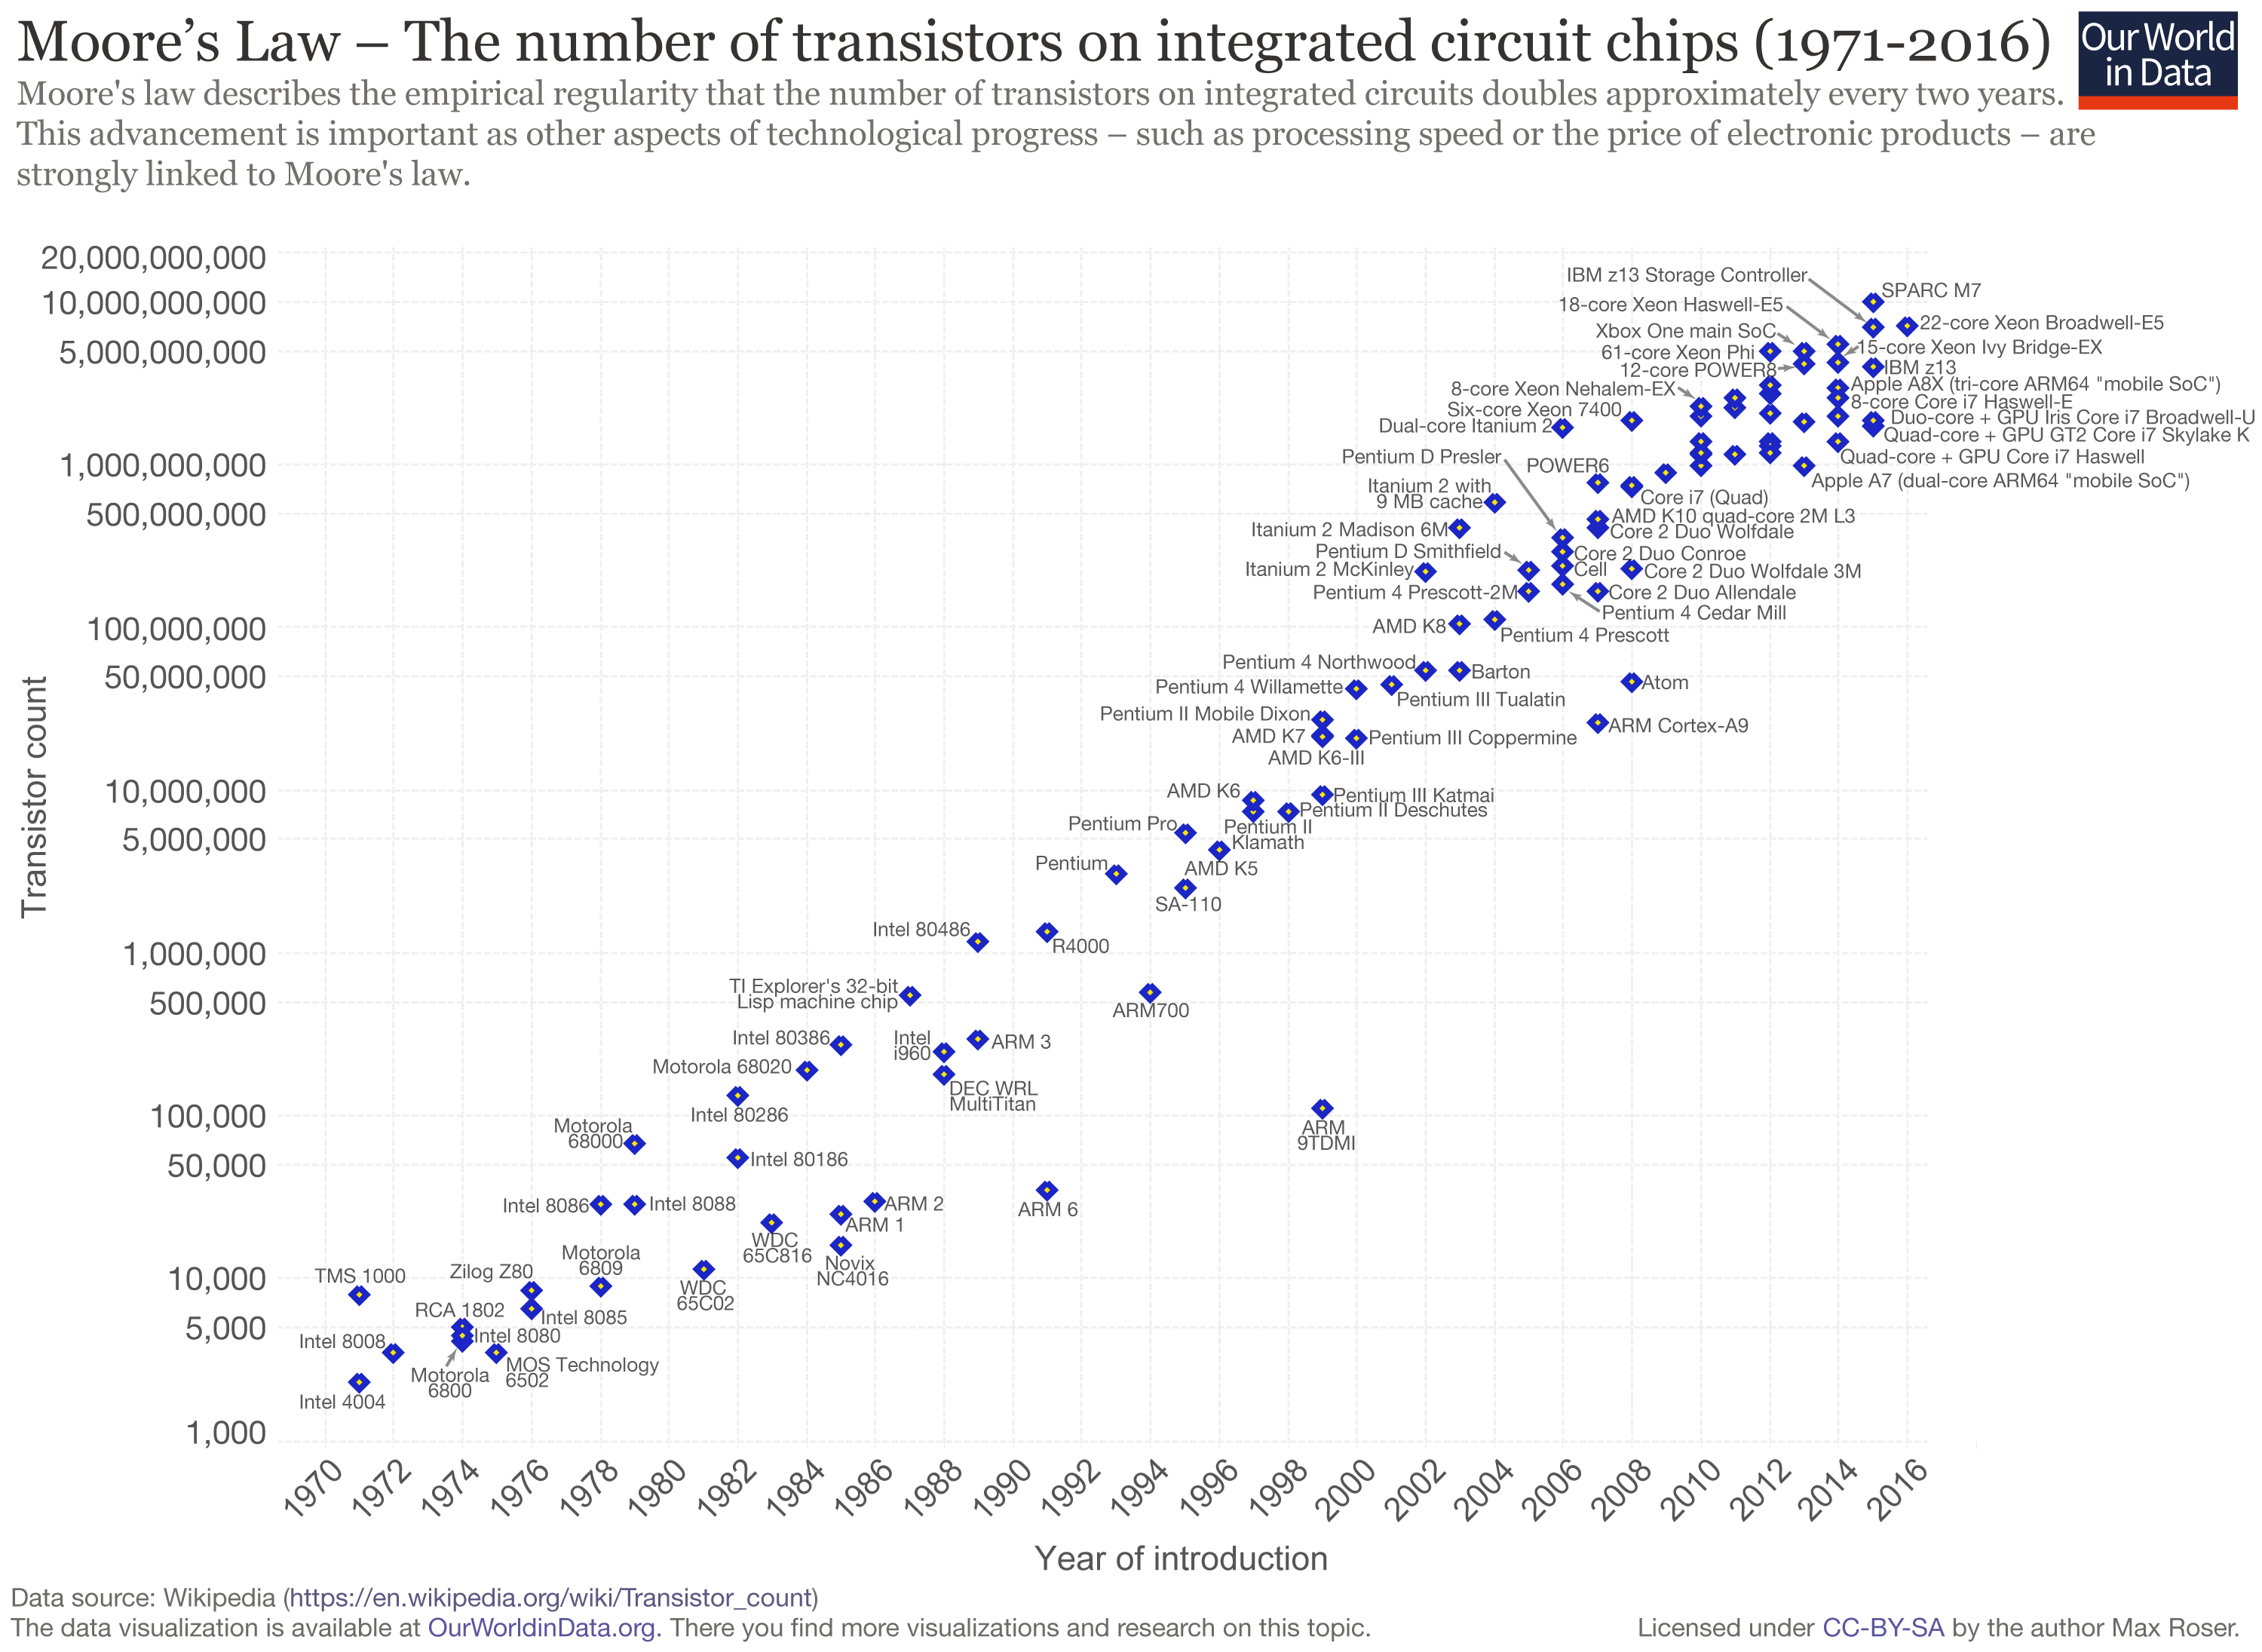
\includegraphics[width=1\linewidth]{pics/moore_law} 
\end{center} 
\caption{Plot of transistor count vs released year for microprocessors\\ \textit{\small{Picture courtesy of Max Roser}}}
\label{tran_count_over_time}
\end{figure}

So it can been seen that transistor count has increased almost in line with Moore's prediction, with some modern CPUs having upwards of 19 billion transistors 
\cite{RN80}. But is an increase in transistor count related to an increase in complexity? Yes, they are directly proportional; by the very definition of complexity, adding more transistors to an IC would increase its complexity. 

For the last few years it has become apparent that the amount of performance increase from each new generation of ICs is not as large as previously. This is due to physical limitations; the silicon wafers are merely nanometres wide already, so they simply cannot be made much smaller
\cite{RN141}. There are also physical limitations in the amount of heat dissipation that can be achieved as well as problems with current leakage. These problems have led to some speculation that Moore's law could be reaching an end 
\cite{RN49}.

\subsection{History of operating systems complexity}

Software, like hardware, has also been growing increasingly complex, driven by a demand that is growing faster than our capacity to design, test, implement and maintain it
\cite{RN85}. Many people have remarked on the steady increase in software complexity and the adverse effects it has on security, maintenance and design costs. Bruce Shneider has written extensively on computer security topics and successfully argues that 'complexity is the enemy of security' 
\cite{RN11} \cite{RN3}. Edward Ogheneovo wrote and interesting paper linking increased complexity to increased maintenance costs for software 
\cite{RN81}. Lawson takes a broader view, talking about the complexity of computer systems as a whole and how software affects that complexity 
\cite{RN55}, as well as the rise in complexity over time. Gelsinger et al. talks about the increase in software complexity driven by the need to keep up with rapid hardware changes while designing microprocessors at Intel 
\cite{RN18}. These papers are discussed more in section \ref{subsec: Complexity as the root cause of modern malware susceptibility} but the salient point linking them is that software complexity is increasing. To further argue this point, a comparison of different versions of popular operating systems is made, as seen in figure \ref{SLOC_windows} and figure \ref{SLOC_linux}. These graphs compare the Source Lines Of Code (SLOC) which is the number of lines of code in the source code before it's compiled. Other metrics were considered, such as the cyclomatic complexity of the source code or the permanent memory space required to install the software. But the availability of the cyclomatic complexity data was lacking and the SLOC was determined to be a more accurate indicator of complexity than the installation size of an operating system. This is partly due to the fact that installation size could be bloated with elements that are not that complex but require a large amount of memory space, such as video, bitmap and audio files. The reason operating systems where considered the best type of software to compare is that they (at least the versions chosen for comparison) are designed for home computers or their modern equivalents and have been is use from the early home computer era until now. 

\begin{figure} \begin{center}
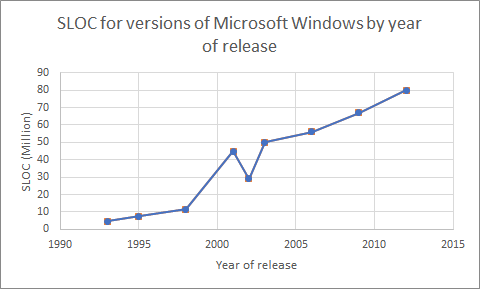
\includegraphics[width=0.8\linewidth]{pics/SLOC_windows} 
\end{center} 
\caption{Source Lines Of Code (SLOC) for different version of Windows operating system vs released year\\ \textit{\small{Data provided by \cite{RN81}}}}
\label{SLOC_windows}
\end{figure}

\begin{figure} \begin{center}
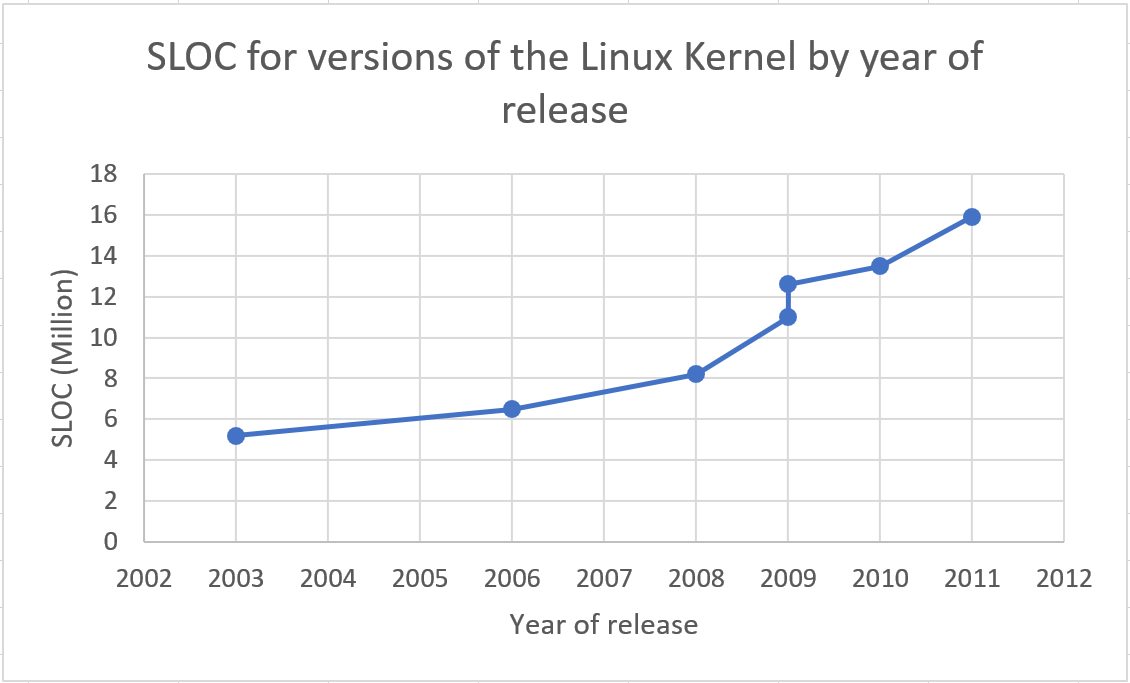
\includegraphics[width=0.8\linewidth]{pics/SLOC_linux} 
\end{center} 
\caption{Source Lines Of Code (SLOC) for different version of the Linux Kernel vs released year\\ \textit{\small{Data provided by \cite{RN81}}}}
\label{SLOC_linux}
\end{figure}

%----------------------------------------------------------------------------------------
%----------------------------------------------------------------------------------------
\section{History of computer insecurity}
\label{History of computer insecurity}
Security is described in \textit{RFC4949 Internet Security Glossary, Version 2} as a system condition where system resources are free from unauthorised access 
\cite{RN66}. In recent years computer security has been a widely discussed topic, mainly due to the damage that malicious programs, or malware, have caused. There are several Standards dealing just with this issue, which shows its importance in modern business and engineering 
\cite{RN70}\cite{RN68}\cite{RN69}. It is now common for companies to lose more from electronic theft than it is from physical theft 
\cite{RN76}. This was not always the case. It seems the inevitable fate of any new successful technology, to be manipulated by malicious actors. Computers and self-reproducing virus programs are both technologies which befell this fate.

Computer security had an interesting beginning. The terms we use today had not be ‘coined’ or where not in common usage, or even are used to mean something slightly different than they do now, such as the computer virus. So to begin, a brief discussion of the origin of some common (by today's standard) phrases.

\textbf{Bug/Debugging:} In 1947 Rear Admiral Grace Murray Hopper noticed the Mark II computer she was using was outputting unexpected results and upon inspection found a moth across a relay, shorting it out 
\cite{RN75}. While the term bug was used in electrical engineering fields, this event is credited with popularising the terms use with computer programmers. A computer system ‘bug’ is an unexpected system behaviour. In this case the relay was shorted out, causing some unexpected behaviour. 

\textbf{Virus:} Fred Cohen first uses the term in his Ph.D. paper, \textit{Computer viruses: Theory and experiments}, published in 1987. 
\cite{RN61}. It followed on from Jon Neuman’s seminal work on self-reproducing automata, Cohen describes a virus as "a program that can ‘infect’ other programs by modifying them to include a possibly evolved copy of itself" \cite{RN61}. Cohen also establishes viruses as a morally neutral technology; meaning it could be employed for good or bad deeds. Cohen mentions several beneficial uses for viruses in the paper, as well as security concern relating to viruses \cite{RN61}. The name virus comes from the fact that the program behaves similar to a biological virus, as it must attach itself to another program, similar to a biological virus attaching itself to another cell. In the time since Cohen's definition, the meaning of a computer virus has changed to mean almost exclusively a form of malware. This change in definition has been encouraged by anti-virus companies, in a bid to help sell their products 
\cite{RN64}. 

\textbf{Worm:} Similar to a virus in that it is a self-reproducing program, the difference come in the fact a worm can execute by itself where as a virus has to attach to another piece of software. Also similar to viruses in that worms are now almost always malware but they first appeared as beneficial programs \cite{RN93}.

\textbf{Malware:} A portmanteau of malicious and software, which aptly describes malware; it is malicious software designed to cause harm. Examples of malware used today are Trojan Horses, Logic Bombs, Key-loggers, Lures, Worms and Viruses.

\textbf{Ransomware:} Also known as a cryptovirus or a cryptoworm. It is another type of malware which encrypts sensitive information and demands payment from the victim to decrypt the data. Payment is normally asked for in e-money such as Bitcoin because it is much harder to trace.
\\

As computer systems have gradually been used to control and store more and more vital information and services, so have the efforts of malicious parties to break into these computer systems for their own benefit. In 1964, AT\& T, a Northern American telecommunications company started monitoring phone calls to catch people illegally using their phone lines to make long distance phone calls for free. This practise involved the use of devices to imitate the tones used by AT\& T to control their phone system. These devices could be an electronic tone generator, a version of which is seen in figure \ref{blue_box} or simply a cassette tape recording of keyboard notes
\cite{RN56}. 1970 saw the first worms created at Xerox's Palo Alto Research Centre. A series of benevolent worms where created to carry out a variety of useful task, such as display messages or use a computer for calculations when it would otherwise be idle. Due to an error, one of these worm programs misbehaved and caused every computer infected with it to crash and on re-starting the computer it would be re-infected and crash immediately 
\cite{RN93}. This event proved the potential for worms to cause massive damage to computer systems and afterwards public research was lacking for several years but it almost certainly continued in secret. In 1986, the Brain virus was found on infected computers in North America. It was designed by two brothers in Pakistan who ran a computer shop, they where worried about pirated copies of their programs and devised the Brain virus as a way to fix this problem. Once infected, a computer would display a message letting the user know they are using pirated software and gave the contact details of the brother's computer shop to get a 'vaccination' 
\cite{RN86}. Worms re-emerged into the public spotlight in 1988 with the now infamous Morris Worm, thought to have infected 10\% of the 60,000 computers predicted to be connected to the internet at the time. It achieved wide spread news coverage becoming infamous. Released on November 2, 1988, the Morris worm effectively brought the internet to a stand still 
\cite{RN90}. There where numerous other worms and viruses created around the same time. These early incidents raised awareness of malware and computer security. Several anti-virus companies formed after these events.

Since the first malware was created, the problem has simple grown. With more and more computer systems controlling important information around the world, the incentive for malicious actors to break into them has grown. As more and more people use computer systems to communicate and organise their daily activities, the incentive for malicious actors to try and deceive people into divulging sensitive information increases. There are now daily reports of malware attacks as well as sophisticated scams run entirely online. While some scams don't involve any malware, but may be simply a deceitful email asking for sensitive information, the definition of security used above is broad enough to cover these cases too. Governments of many countries now employ computer security experts to help protect themselves, as well as developing malware to use against their adversaries. A well known example of a  government-made malware is the Stuxnet virus. Stuxnet was found on an infected computer in 2010 by Sergey Ulasen. Ulasen ran a small computer security firm and a client was seeking help with a computer stuck in a reboot loop. This triggered a massive investigation by several companies which lead to the conclusion that Stuxnet was a targeted malware designed to hinder Iran's nuclear enrichment capabilities. The target as well as the amount of effort that went into Stuxnet, lead many to believe it must have been a state-sponsored malware attack, with Israel and the USA being the most likely culprits 
\cite{RN91}\cite{RN92}. The Stuxnet virus was also interesting because it was the first case of a malware 'in the wild' being used to cause physical damage, where as the harm caused by other malware seen before it was limited to computer systems. Stuxnet virus was designed to attack PLC controllers connected to frequency converter drives in one specific nuclear enrichment plant in Iran. Once these PLCs were identified, Stuxnet would then routinely run the drives at frequencies that would cause them to break. There are many, many, many more examples of malware and computer security issues, with more happening each day. Its worth noting that there has been a general trend of malware being used to steal money, the first malware seemed to have been created out of curiosity and now more often than not malware is being used to steal money or valuable information which can be sold to other criminals. The WannaCry ransomware being a salient recent example of modern malware being created to steal money 
\cite{RN94}. 

\begin{figure} \begin{center}
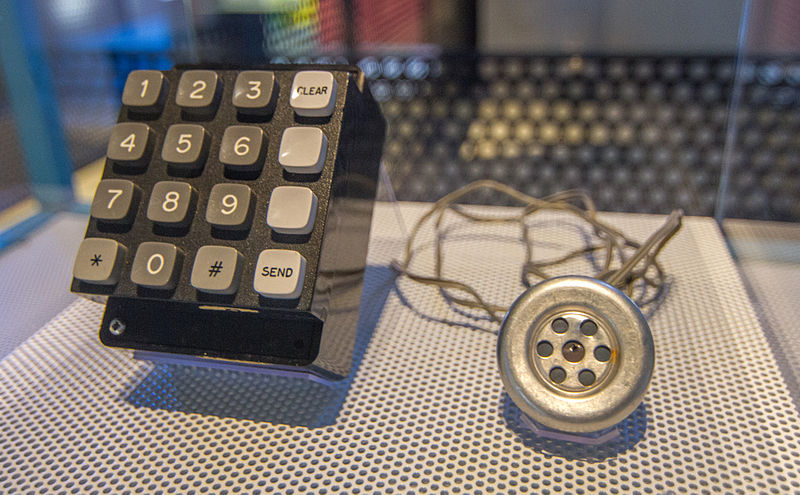
\includegraphics[width=0.8\linewidth]{pics/blue_box} 
\end{center} 
\caption{A Blue Box; electronic tone generating device used to gain access to AT\& T's phone network in North America\\ \textit{\small{Picture courtesy of Maksym Kozlenko}}}
\label{blue_box}
\end{figure}


\subsection{Complexity is the root cause of modern malware susceptibility} 
\label{subsec: Complexity as the root cause of modern malware susceptibility}
There is one common aspect linking each and every case of computer security being breached, they all use some vulnerability within the computer system (the system being inclusive of the users) to gain access they shouldn't have. These vulnerabilities can be in the software, hardware or even in the users choice or password or their habits (use of USB drives, physical security of their computer etc.). In the examples listed in section \ref{History of computer insecurity}, AT\& T had a vulnerability in their phone system in that anyone could control the system through the use of tones played down the line. It can be guessed that the idea that malicious actors would attempt do this this was not considered likely or considered at all when the system was first designed. The Brain virus exploited vulnerability found in MS-DOS operating system, which was new at the time \cite{RN86}. The Morris worm exploited weak passwords as well as vulnerability with in Unix's sendmail, fingerd and rsh/rexec commands 
\cite{RN86}. Stuxnet exploited four zero-day vulnerabilities, which is unprecedented and one of the reasons it is believed to be a state-sponsored malware\cite{RN91}. A zero-day vulnerabilities is a vulnerabilities that is not publicly known; the software manufacture is unaware of it. WannaCry exploited a flaw in the Windows operating system \cite{RN94}. So it can be concluded that malware needs a vulnerability to exploit if it is going to gain unauthorised access to a computer system. So what is a vulnerabilities?, what causes them? and how can they be avoided? These are all logical questions that follow. 

A vulnerability can be described as a way to let unauthorised actors enter a computer system, which is perhaps not that illuminating in terms of explaining what it is. This is because vulnerabilities can have so many forms, ranging from hardware design flaws such as the type that caused the Meltdown and Spectre exploits to be possible \cite{RN16}, to software flaws such as the type exploited by Stuxnet and WannaCry \cite{RN91}\cite{RN94}. There could be vulnerabilities in the users selection of password, as exploited in the Morris worm \cite{RN86}. Users can also provide other vulnerabilities in there use of external media they connect to the computer system as well as the physical security of devices connected to the computer system. This was the case with Stuxnet, as it is believed to have entered the target computer network from a USB storage device, as the computer network in question was isolated from the internet \cite{RN91}. So vulnerabilities are varied and many in their forms, but what causes them? and how can they be avoided?

So vulnerabilities are way to access a computer network through means that shouldn't be possible in a ideal world. And it follows that these vulnerabilities are only possible if they are never found or thought of by the designers and/or manufacturers and then fixed. So what would make it hard for the designers to find the aforementioned vulnerabilities? Well, if the task is simply too large, the design so complex, it's simply too hard to consider every possible avenue of access into the computer system. As talked about earlier in section \ref{The progressing complexity of computer hardware and software}, software and hardware have both been continually getting more complex to meet our demand for more functionality, power and convenience. This complexity will almost certainly lead to more vulnerabilities.

Bruce Shneider has extensively talked about what he calls a truism; that "complexity is the worst enemy of security" \cite{RN96}. Scheider first mentioned this in 1999, in his security blog \cite{RN3} and has since talked about it in at least two of his books \textit{Secrets and Lies} (2000) and \textit{Practical Cryptography} (2003) as well as in various articles and interviews. Shneider convincingly argues that good security come from getting everything right: careful analysis of source code, specifications and systems. A more complex system will require more detailed and expensive analysis, with greater chance of a vulnerability being overlooked, as there is simply more to look at. The more complex a system is: the more lines of codes make up said system, the more interactions with other systems it has, the more configuration options available and the more vulnerabilities there are. With a complex system there is more to get wrong and good security require that everything is done correctly.

Edward E. Ogheneovo wrote an illuminating paper titled \textit{On the Relationship between Software
Complexity and Maintenance Costs} in 2014. In the paper he claims software is increasing in complexity and an increase in complexity drives up the cost of maintaining the software. He successfully links  maintenance costs to the amount of bugs in the software and shows that the root cause of the bugs is complexity \cite{RN81}. 

While working at Intel during the turbulent 1980's to 2010, Patrick Gelsinger, Desmond Kirkpatrick,
Avinoam Kolodny, and Gadi Singer witnessed first-hand the increase in complexity, both in hardware being designed by themselves as well as the CAD software created to facilitate the design process. They provide an excellent recounting of this period at Intel in the paper \textit{Such a CAD!}. They illustrate clearly what is driving this increase in complexity: demand \cite{RN18}. Customers demand and expect more powerful computer products in line with Moore's Law, this is not to say most customers where aware of Moore's Law, but they where aware (within a few years of the home computer era) that computers continually got more powerful. If Intel didn't meet this demand, others would have and Intel would not have been as successful in business.

Going back to 1987 and Fred Cohen's seminal paper \textit{Computer viruses: Theory and experiments}. Cohen comes to the conclusion that the sharing of information needed in a general purpose computer, such as a home computer or PC, is in direct opposition to the goals of viral security. Which is implying that computer systems where are already becoming too complex in relation to viral security in 1987.

With all this in mind, it can be said that the root cause of malware susceptibility and computer insecurity is complexity. Which leaves the question, what can be done about it? This question is beyond the scope of this thesis but a possible answer is given in in section \ref{History of the MEGA65 project}, an open-source simple computer.
 
%%Chapter 3 - Case studies of retro computing projects
%	What does the retro computing revival project productization process look like?
%	What risk and challenges are assosiated with a retro computing revival project?


\chapter{Case studies of retro-computing projects}
\label{Chapter3}
This chapter forms a body of knowledge on retro-computer projects which are attempting to release a new product to market. This is achieved through a series of case studies into several retro-computer projects. Each case study extracts the process the project followed in releasing a new product to market. The case studies also highlight any challenges the projects faced during the productization process. 

For each case study there is a brief description of the product and the team behind it. Any information about the productization process or challenges faced during that process is recorded. From this record, a list of the process steps is extracted, as well as a list of challenges the project faced. The challenges are then categorised into risk types for each case study. At the end of the chapter the separate case study processes are combined into a list and then illustrated, see Figure \ref{case_study_process}. The separate case study risks are combined into a risk table and ranked according to the potential damage they could cause. 

%----------------------------------------------------------------------------------------
%----------------------------------------------------------------------------------------
\section{Open-source case studies}
Despite not being retro, the Arduino and Raspberry Pi where both studied because of their open-source nature and their market success. The Raspberry Pi is also influenced by retro ideas from the home computer era, such as booting straight into a programming environment as well as the creators being inspired by the BBC Micro, from the home computer era.

%%%%%%%%%%%%%%%%%%%%%%%%%%%%%%%%%%%%%%%%%%%%%%%%%%%%%%%%%%%%%%%%%%%%%%%%%%%%%%%%%%%%%%%%%%%
\subsection{Arduino}
\textbf{What is it?}\\
Arduino is a company which designs, produces and sells the Arduino range of single-board microcontrollers as seen in Figure \ref{ArduinoUno3}. These are mostly 8-bit machines with 32-bit machines being introduced later and are known for being inexpensive to purchase. The Arduino company has released all the hardware designs as open-source under a Creative Commons licence. The associated IDE (Integrated Development environment) software is also open-source and Arduino also encourage and facilitate a community of hobbyist, open-source enthusiasts and professionals 
\cite{RN133}. \\

\textbf{When was it produced?}\\
The first Arduino board was designed and made available to students at the Interaction Design Institute Ivrea (IDII) in Italy in 2005. As word spread, the board quickly became popular outside of the class and Arduino boards remain hugely popular today 
\cite{RN103}.\\

\textbf{Why was it produced?}\\
It was used to help teach the students at IDII interactive design (also known as physical computing). A co-founder of Arduino, Massimo Banzi was using another commercially available microcontroller called the BASIC Stamp to teach his class prior to the Arduino board or its inspiration, Wiring being created 
\cite{RN103}. Banzi found the Stamp didn't meet his needs for teaching and it was too expensive for the students. Banzi decided to design his own microcontroller and associated IDE to create an entire platform for users to easily achieve their goals. Banzi drew heavy inspiration from another very similar project called Wiring that was also in development at IDII before and during the creation of the first Arduino board. Wiring in turn built on another related project, Processing, which provided the starting point for the IDE used in Wiring 
\cite{RN110}\cite{RN135} \cite{RN111}. \\

\begin{figure} \begin{center}
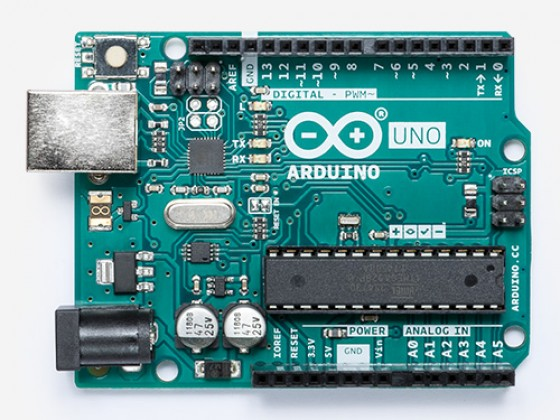
\includegraphics[width=.3\linewidth]{pics/Arduino_uno_3} 
\end{center} 
\caption{Arduino Uno Rev 3\\ \textit{\small{Picture from \url{https://store.arduino.cc/usa/}}}}
\label{ArduinoUno3}
\end{figure} 

\textbf{Process}\\
Arduino started with an idea, to create a cheap microcontroller for students and an accompanying platform to make it easy to use. From the idea stage, then a prototype was built. The prototype in this case is taken to be the microcontroller board and accompanying software Massimo Banzi and David Cuartielles developed in 2005 
\cite{RN111}. This prototype had a somewhat convoluted history, being derived from Wiring, another similar project created by a student for their thesis project 
\cite{RN110}\cite{RN111}. It's worth noting that the software or Integrated Development Environment (IDE) was (and still is) open-source and several others helped in its development, up to and after the prototype stage. Banzi and Cuartielles invited others to help with the project, an advisor Tom Igoe, a student David Mellis to help write the software and Gianluca Martino who could help facilitate the production of the board 
\cite{RN111}. After discussions with Igoe, the Arduino team decided at some point in 2005, that the target market for their product was much larger than just the students in there respectively schools. The prototype then went into a period of refinement, with the main goals of making it cheap to produce and simple to use. This included fixing some bugs in the hardware design 
\cite{RN111} and more extensive work on the IDE to included more user-friendly features. The software and hardware was also modified allow support for a cheaper chip, which is the microcontroller at the core of the Arduino board.

The Arduino team decided to produce a batch of 200 units with a prearranged agreement with two schools to buy 50 units each. The agreement meant to production run would atleast make back half of its cost, even if the other 100 boards were not sold. This reduced the risk to investors (which were Arduino team members in this case). This small production run was meant as a test to see if there was market interest in the product outside of the schools. The team then placed some paid advertisements marketing the Arduino board, as well as discussing the product with friends and colleges to spread word of mouth 
\cite{RN111}. The Arduino boards started to sell, slowly at first but it was obvious at this point that there was a market for the Arduino board.

As the Arduino is a single-board device with no case or human interface device (HID), the hardware process from working prototype to finished design was relatively simple. It consisted of just the electronic board design and parts selection with regard to price, quality and availability. A manufacturer had already been found, Smart Projects, whom was owned by Arduino team member Gianluca Martino. There was also associated software actively being worked on during the period the hardware was being refined for the production run of 200 boards mentioned earlier.

The fact that Arduino creators didn't know if half of the first production run would sell, and if it did, who would be interested in it, leads to the idea that they didn't do a lot of market research before hand. The team thought of the first production run as a test to gauge market interest
\cite{RN111}. \\

\textbf{Steps Identified}
\begin{enumerate}
\item Construct a working prototype to fulfil an idea or need.
\item Decide final product features and specifications based on prototype feedback.
\item Refine prototype to remove bugs/errors and add any features that are required for the product launch.
\item Add team members as needed to help grow the project. Focus on what skills they can provide when deciding on members.
\item Self fund a small production run of the final product.
\item Place advertisements and use word of mouth to spread awareness of the product.
\item Partner with or form agreements with distributors to increase the availability of the product.
\end{enumerate} 

\textbf{Challenges faced during productisation and beyond}\\
The biggest challenge for the Arduino company was simultaneously making a profit for the company while being open-source with their products and allowing anyone to manufacture and sell them. Arduino handled this successfully, with both the designs still being open-source and the company (Arduino LLC) still trading but as it is a private company it doesn't need to publish earnings so they could not be scrutinised. The original decision to make the designs open-source, according to Banzi 
\cite{RN111} \cite{RN103}, stemmed from the realisation that IDII was running out of money and would shut within a few years, potential endangering the Arduino project. Hernando Barragán, the creator of Wiring, claims Banzi didn't have a choice and had to make it open-source. This was because Arduino used work from the Wiring and Processing projects and both of them are open-source and require any derivative to also be open-source 
\cite{RN110}. The Arduino team partnered with a manufacturer and got the first boards produced and sold for a small profit. Arduino found that as they were the first to market (with good reason) that they still sold a lot due to lack of competition, which was a possibility considering the open-source nature of the project. But when cheaper copies started being manufactured in Taiwan and China, this initially had the effect of increasing the sales through Arduino, even though there were cheaper versions available. Arduino put this down to the competition being of a lesser quality at that time 
\cite{RN113}. Arduino also charge a fee if other producers wanted to use the Arduino name. As the market matured, Arduino expected other producers and manufactures to be able to produce the Arduino boards at a cheaper price and of similar quality, which has happened. The Arduino company now focuses more on selling their expertise as the inventors, consultancy work, enabling the Arduino community and designing and selling Arduino accessories, such as 'shields', plug in devices that add extra functionality to the Arduino range 
\cite{RN113}.\\

The other big challenge Arduino faced was from legal challenges around ownership of the Arduino Trademark. In 2009, after the initial success of the Arduino boards, the co-founders decided they needed to create a company to hold all the trademarks and created Arduino LLC in the USA, as well as trademarking the name Arduino in the USA. It was decided to focus on the USA first, but one of the team members that was working on the production of the existing Arduino boards, separately registered the Arduino trademark in Italy without telling the rest of the Arduino team until 2014. In 2014, the company which held the Italian trademark and manufactured Arduino boards, Smart Projects, hired a new CEO. Smart Projects then changed its name to Arduino SRL and stopped paying Arduino LLC royalties for using the Arduino name 
\cite{RN115}. What followed was a drawn-out legal and community battle for a couple of years. In October 2016 the two parties announced an agreement to join forces and cooperate moving forward
\cite{RN116}. The schism seems to have come from two different parts of the initial group wanting to take the company in different directions, the production team wanting to keep production in Italy and the others wanting to expand into USA and China and let many other manufactures in. \\

A minor challenge the Arduino team faced was from attacks on their integrity from people that didn't like the way Banzi treated Hernando Barragán in regard to using his open-source work to create Arduino. The perceived slight was not from the use of the open-source code, which is by definition free to use, but from the fact that Banzi chose to fork and use the code without asking Barragán to be part of the Arduino team. Barragán was a past student of Banzi and they worked closely together during Barragán's creation of Wiring for his master's thesis project. Barragán also had plans to make the Wiring board compatible with cheaper microcontrollers (the chip at the core of the Arduino and Wiring boards) which is the work Banzi and team did shortly after forking the code from Wiring.\\

\textbf{Relevant useful lessons gleamed from the study}
\begin{enumerate}
\item Open source hardware can make a profit in the short term by being first to market.
\item Open source businesses can generate profit in other ways including: consultation or selling expertise of the product, licence fees for use of trademark such as Arduino did with their name as well as designing and producing accessories.
\item It is extremely important to keep control of trademarks and other intellectual property (IP).
\item Open-source projects encourage others to participate simple by being open, this in turn creates a community of people, these open-source communities seem to naturally converge around the original creator(s). The original creator of the Linux kernel, Linus Torvalds and the communities around Arduino and Raspberry Pi are other examples of this. The original creator(s), by being the focal point, should generally be well informed on what the community is doing, this can be leveraged by hosting community-oriented services, such as forums to share ideas and knowledge which in turn should increase the popularity of the product. \\
\end{enumerate}

\textbf{Challenges faced}
\begin{enumerate}
\item Open-source business model
\item Legal challenges to ownership of Arduino trademark
\item Attack on integrity from use of open-source work
\end{enumerate}

%%%%%%%%%%%%%%%%%%%%%%%%%%%%%%%%%%%%%%%%%%%%%%%%%%%%%%%%%%%%%%%%%%%%%%%%%%%%%%%%%%%%%%%%%%%%%%%%%%%%%%%%%%%%%%%%%%%
\subsection{Raspberry Pi}
\textbf{What is it?}\\
A cheap, open-source, single-board computer which runs a version of the Linux operating system shown in Figure \ref{Raspberry_Pi}. The first version had a 32-bit processor with later version including a 64-bit processor.
\cite{RN99}.\\

\textbf{When was it produced?}\\
The Raspberry Pi version 1 Model B was first sold in February, 2012 for \$35, with Model A coming out soon after for 25 USD 
\cite{RN100}.\\

\textbf{Why was it produced?}\\
In 2006, Eben Upton, who grew up using a BBC Micro (from the early home computer era), had a desire to help kids learn computer science and related topics. He compared the BBC Micro on which he learned, which booted up straight into a BASIC command prompt, to modern devices children have access to, such as a tablet. He lamented that a child with a tablet is so far removed from the inner workings of the device that learning computer programming and related skills is a lot more difficult 
\cite{RN97}. To achieve his goal of helping kids learn about computers, Upton decided to make a small, cheap computer which would hopefully encourage kids to play and learn, as he did with the BBC Micro. Upton and several others formed a charity in 2009 with the purpose of advancing this agenda, called The Raspberry Pi Foundation. It wasn't until a few years later that Upton found a suitable chip for the Raspberry Pi. While working for Broadcom on the design team for the BCM2835 chip, Upton realised the BCM2835 would be perfect for the Raspberry Pi computer he had envisaged
\cite{RN97}.\\

\begin{figure} \begin{center}
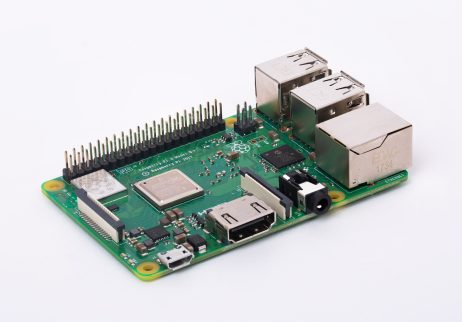
\includegraphics[width=.3\linewidth]{pics/Raspberry_Pi_3B+} 
\end{center} 
\caption{Raspberry Pi 3 Model B+\\ \textit{\small{Picture from \url{https://www.raspberrypi.org/products/}}}}
\label{Raspberry_Pi}
\end{figure} 

\textbf{Process}\\
The Raspberry Pi first started with a desire to help children engage with computers and computer topics. Eben Upton, one of the founders of the Raspberry Pi Foundation, decided the best way to achieve this was to give them access to a cheap computer that they could ``mess around''  with and learn along the way, much as he did with a BBC Micro when he was young 
\cite{RN98}. Upton built several prototypes while trying to achieve this goal. The first was built in 2006 using a microcontroller as the core and gave about the same computational power as a BBC Micro 
\cite{RN137}. Upton originally thought a highly-integrated remake of the BBC Micro would meet his goal but after discussion with like minded people, Upton abandoned this in favour of a more powerful machine 
\cite{RN98}. Upton team-up with other like minded individuals in 2009 and formed the Raspberry Pi Foundation with the stated goal to ``put the power of computing and digital making into the hands of people all over the world.'' 
\cite{RN138}. Upton and the rest of the foundation now faced the problem that all the microprocessor available at the time were too expensive to include in a computer which needed to be cheap. It wasn't until a couple of years later that Upton found a suitable chip, the Broadcom BCM2835, a System-on-Chip (SoC), which is a complete microcomputer within a chip. In 2011, the Raspberry Pi Foundation had made a new prototype, with the BCM2835 at its core. This new prototype was shown publicly in May 2011 and received a huge amount of attention 
\cite{RN140}. In this somewhat unplanned showing, the Raspberry Pi team said they would have it finished by May 2012 and it would cost \pounds 15. This self-imposed deadline put some pressure on the team to finish by their publicly stated date.  

Over the few months the prototype design was refined, with the goal of trying to keep the board within \$35 USD. During this process several features were cut to save costs 
\cite{RN98}. Upton also embarked on a campaign to secure parts at a cheap as a possible price 
\cite{RN98}. A version of the Linux OS, designed specifically for the Raspberry Pi, was also in development 
\cite{RN98}.

Once the team had the designs for the final product agreed upon, they originally planned to make 1000 unit in the first production run to gauge the market
\cite{RN139} but after the May 2011 showing received so much attention, they revised the initial run to 2,000 units 
\cite{RN98}. The funds for the original production came from donations from the trustees of the Raspberry Pi Foundation 
\cite{RN142}. The Raspberry Pi team then had to find a manufacturer and ended up finding an outfit in China which could make the raspberry at a decent price 
\cite{RN98}. Not long after securing this initial run in 2011, the raspberry pi team realised they had more demand for units than they could secure funds to manufacture, they estimated 10,000 units would need to be made for the launch. To help solve this problem, the Raspberry Pi team partners with two large companies right before the product launch, Element14 and RS. They both agreed to distribute and manufacture the Pi, so the Raspberry Pi team pivoted at this point to becoming a designing and licensing business and not a manufacturer of the Raspberry Pi 
\cite{RN98}. This partnership secured worldwide distribution and manufacturing channels, something the Upton is very proud of as he says it let the Raspberry Pi grow a lot faster 
\cite{RN98}.\\

\textbf{Steps Identified}
\begin{enumerate}
\item Construct a working prototype to fulfil an idea or need. This prototype is taken as the first with a Broadcom chip, shown publicly in May 2011.
\item Form foundation or other body to hold licenses and other IP.
\item Add team members as needed to help grow the project. Focus on what skills they can provide when deciding on members.
\item Decide final product features and specifications based on prototype feedback.
\item Refine prototype to remove bugs/errors and keep of end product cost down. Develop software needed for launch, OS and applications.
\item Get agreements for parts at acceptable prices from suppliers.
\item Launch website and have online presence, try to generate awareness through media.
\item Self fund a production run of the final product, 2000 units.
\item License out product to larger companies which can make and distribute the product better and faster
\end{enumerate} 
 
\textbf{Challenges faced during productisation}\\
The Raspberry Pi productisation process seems to have avoided most major problems, how much of this can be attributed to Upton waiting for a chip that suited the project is hard to decipher, but it most definitely helped. Whether waiting for a suitable chip is a challenge or not depends on the project.
The Raspberry team announced a release date before the final product was ready, this added a lot of pressure during that window to meet their self imposed deadline but may have helped push the project along at a faster pace 
\cite{RN97}. 
The Raspberry Pi was delayed in the first production run due to compliance laws in Europe around electronic interference compliance. The Raspberry Pi needed to be tested for electronic interference but the creators didn't realise this until it was too late to avoid delays 
\cite{RN98}. The Foundation wanted to keep the cost of a board to \$35 as they believed it would be critical to achieving their goal of allowing as many people as possible to afford one. To keep the cost down, Upton had to cut several features during the development phase 
\cite{RN98}. Upton also embarked upon an aggressive campaign to secure parts at low cost 
\cite{RN98}.\\

\textbf{Relevant useful lessons gleamed from the study}
\begin{enumerate}
\item Open source hardware can be incredibly popular. 
\item Check relevant laws and seek expert advice early as possible to avoid delays in production.
\item Keeping the cost down can greatly increase market size and device uptake. \\
\end{enumerate}

\textbf{Challenges faced}
\begin{enumerate}
\item Regulatory compliance
\item Strict product criteria on cost
\end{enumerate}

%----------------------------------------------------------------------------------------
%----------------------------------------------------------------------------------------
\section{Retro-computing case studies}
These case studies look at a group of products that are inspired by 8-bit computers from the home computer era mentioned. Two of the biggest names from that time, Spectrum and Commodore are both reproduced in modern revival projects which are studied in this section. These projects are retro revival and 8-bit so they are perfect for case studies.

%%%%%%%%%%%%%%%%%%%%%%%%%%%%%%%%%%%%%%%%%%%%%%%%%%%%%%%%%%%%%%%%%%%%%%%%%%%%%%%%%%%%%%%%%%%
\subsection{Sinclair ZX Spectrum Vega}
\textbf{What is it?}\\
The Sinclair ZX Spectrum Vega is a game console inspired by the ZX Spectrum (another hugely popular home computer from the early home computer era,  which was released in the United Kingdoms in 1982 by Sinclair Research. The ZX Spectrum Vega comes preloaded with 1000 games, most of which were written for the original ZX Spectrum. It swaps the full keyboard of the original for a directional thumb pad and 9 rubber buttons as shown in Figure \ref{Spectrum_Vega}. It has the endorsement of Sir Clive Sinclair, the founder of Sinclair Research. The Vega was created by Retro Computers and uses a hardware design created for the project and has a microcontroller at its core and custom-built software to allow it to play all games written for the ZX Spectrum 
\cite{RN119}.\\

\textbf{When was it produced?}\\
The Vega was released in April 2015, following a successful crowd-funding campaign on Indiegogo, a crowd-funding service. It cost \pounds 100  at launch but is no longer produced or sold by Retro Computers as they have run into financial and legal troubles relating to another product, the Vega+ and was recently wound up 
\cite{RN120}.  \\

\textbf{Why was it produced?}\\
The Sinclair ZX Spectrum Vega was a commercial endeavour. \\

\begin{figure} \begin{center}
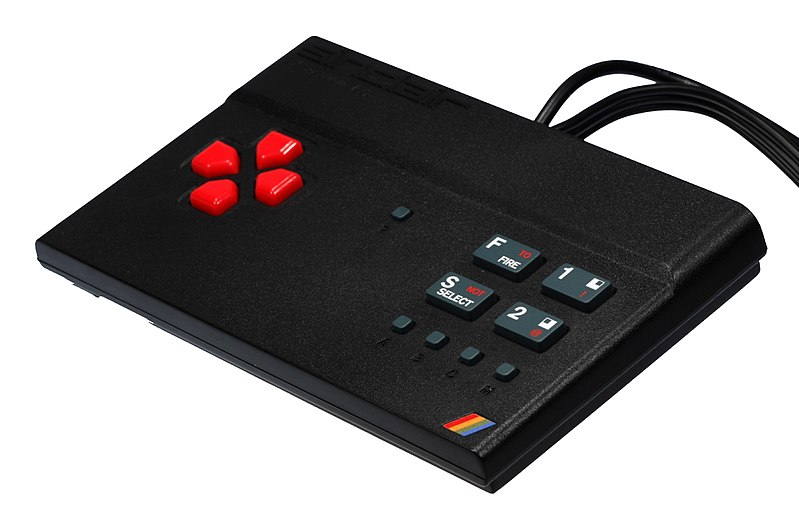
\includegraphics[width=.3\linewidth]{pics/Spectrum_Vega} 
\end{center} 
\caption{Sinclair ZX Spectrum Vega, a game console with 1000 preloaded games inspired by the ZX Spectrum from 1982. \\ \textit{\small{Picture courtesy of Marco Tangerino}}}
\label{Spectrum_Vega}
\end{figure} 

\textbf{Process}\\
\label{Vega process}
The Sinclair ZX Spectrum Vega first came to public attention due to a crowd-funding campaign launched by it creators Retro Computer (RCL) on Indiegogo in 2014. The campaign was intending to raise the capital needed manufacturer the first production run of the Vega. The campaign was successful, raising 149\% of their intended goal or \pounds 155,682. Retro Computers Limited (RCL) claimed in the campaign that the design was complete already and that RCL had agreements in place to use the Sinclair brand as well as the rights to use 1,000 games that would be shipped with the Vega. The terms of the agreement with the games rights holders was that RCL can distribute the games on the Vega but for each Vega sold a donation must be made to a charity for 10\% of the Vega purchase price. To secure the rights to use the Sinclair name, Paul Andrews, the managing director of RCL at the time, reached out to Sir Clive Sinclair to seek his approval, which was forthcoming with the provision that David Levy be able to join RCL and provide oversight on behalf of Clive. Once the crowd-funding campaign had secured funding, RCL went about finding a manufacturer and in January 2015 they announced they had formed an agreement with SMS Electronics Ltd to manufacture the Vega. Later the same month RCL announced that they have received suggestions on how to improve the Vega from various parties and they would be implementing two of them: adding extra buttons and adding an hardware interface and ability to upgrade the software. RCL also noted that the Vega had passed the required ECM (Electromagnetic compatibility) test in June 2015. Later the same month RCL posted on the Indiegogo campaign page that the first production run of the Vega had been complete but they could not legally send them to backers yet as they first needed a PEGI (Pan European Game Information) age rating. RCL announced that the first batch of Vegas were sent to backers on the 7th of August 2015.\\

\textbf{Steps Identified}
\begin{enumerate}
\item Construct a working prototype to fulfil an idea or need, in this case it was basically feature complete and finished, this included the electronics design as well as the tooling and case designs and software. 
\item Form agreement with relevant license or rights holders to use their IP.
\item Launch crowd-funding campaign to raise capital for first production run.
\item Find and form agreement with manufacturer(s) to produce product.
\item Refine prototype based on community suggestions.
\item Organise to have product tested as required by relevant laws. The Vega needed to pass an ECM test and a PEGI age rating test.
\item Launch website to sell product and have an online presence.
\item Send out finished product to backers.
\end{enumerate} 

\textbf{Challenges faced during productisation}\\
The Indiegogo campaign was successful, raising 149\% of the funding goal 
\cite{RN119}. 
Retro Computers launched a crowd-funding campaign offering a product to backers which wasn't complete yet, since this campaign, there has been a successful legal challenge that states that this type of agreement is a sales contract and such they are legally obliged to deliver the product regardless of problems that could arise before the product is complete 
\cite{RN122}. This ruling came from legal action against the Indiegogo crowd-funding campaign for next iteration from Retro Computers the Sinclair ZX Spectrum Vega Plus console. So by offering a product to backers in a crowd-funding campaign, Retro Computers exposed themselves to extra risk and it may have been better to word the crowd funding campaign differently to avoid this or just not offer the product to backers at all but rather sell it to them cheaper once it is finished (if it gets finished).\\

\textbf{Relevant useful lessons gleamed from the study}\\
Crowd-funding campaigns can be useful to raise capital but offering a as-yet unfinished product to backers exposes the campaign founders to an amount of risk in that they legally have to deliver the product and there may be unforeseen costs and challenges in producing it.\\

\textbf{Challenges faced}
\begin{enumerate}
\item Crowd-funding campaign to deliver product that had not been finished
\end{enumerate}

%%%%%%%%%%%%%%%%%%%%%%%%%%%%%%%%%%%%%%%%%%%%%%%%%%%%%%%%%%%%%%%%%%%%%%%%%%%%%%%%%%%%%%%%%%%
\subsection{Spectrum Vega+}
\textbf{What is it?}\\
The follow up of the Sinclair ZX Spectrum Vega mention earlier. It is, like it predecessor, inspired by the Sinclair ZX Spectrum and also has the endorsement of Sir Clive Sinclair, although it is reported he has very little to do with the actual running of Sinclair Research 
\cite{RN123}. The Vega Plus is a hand-held console with its own screen and internal battery as well as the ability to output its display to a TV, although this feature couldn't be made to work in a review of the Vega Plus 
\cite{RN117}. The Vega+ has a microcontroller at its core which provides the computational power 
\cite{RN143}.\\

\textbf{When was it produced?}\\
In July 2018, Retro Computers sent out a number of Vega Plus consoles to backers. No other Vega Plus consoles have been produced.\\

\textbf{Why was it produced?}\\
Like its predecessor, the Vega Plus was a commercial endeavour. \\

\begin{figure} \begin{center}
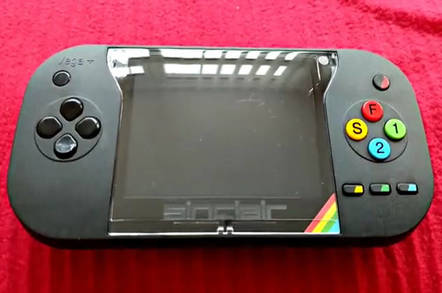
\includegraphics[width=.3\linewidth]{pics/Spectrum_vega_plus} 
\end{center} 
\caption{Sinclair ZX Spectrum Vega Plus console, the poorly received culmination of a tumultuous crowd-funding campaign  \\ \textit{\small{Picture courtesy of Craig Wootton}}}
\label{Spectrum_Vega_Plus}
\end{figure} 

\textbf{Process}\\
The Spectrum Vega+ was the next product offered by Retro Computers Limited (RCL) after the Spectrum Vega, mentioned above in section \ref{Vega process}. Like the Vega, the Vega+ used a crowd-funding campaign on Indiegogo to raise capital to fund the first production run of 2,500 units and prepare for the second production run 
\cite{RN143}. When the campaign was launched on 15th February 2016, RCL claimed they had a working prototype of the Vega+ and supplied video evidence to back up this claim 
\cite{RN145}\cite{RN143}. The campaign closed on the 27th of March 2016 having successful reached its target; it raised 366\% of the target or \pounds 512,790. 
But not long after the end of the campaign, two of the directors of RCL resigned citing ``irreconcilable differences'' between them and the remaining directors
\cite{RN146}. One of the directors, Chris Smith, was also the creator and owner of the firmware which was created to run the Vega+, when he left he took the rights to use them with him and refused RCL the rights to use it in the upcoming Vega+. This proved to be a difficult situation for RCL to recover from while under the leadership of the sole remain director, Dr David Levy. RCL eventually released a small number of the Vega+ consoles to no more than 400 of the over 4,500 backers of the campaign after Indiegogo threatened to send debt collectors after RCL to recover the funds unless backers received a Vega+ 
\cite{RN147}. RCL has now been wound-up by creditors demanding payment and no more Vega+ consoles are ever likely to be made, leaving thousands of backers without the product they paid for and hundreds of thousands of pound unaccounted for 
\cite{RN120}\cite{RN148}. By almost any metric it can be said the Vega+ project was an abject failure and such the process they used will be of little value. \\

\textbf{Steps Identified}
\begin{enumerate}
\item Construct a working prototype to fulfil an idea or need.
\item Launch crowd-funding campaign to fund first production run and prepare for second run
\item Lose rights to use prototype from first point, forced to remake the firmware because of this.
\item Add team members as needed, Levy brought in two new directors after Smith and Andrew resigned.
\item Make promises to backers about the imminent delivery of the product but don't deliver, this happened numerous times after the end of the crowd-funding campaign, which was during the development of the Vega+ with the new firmware.
\item Release a very small number of units to some backers after multiple threats of debt collectors from Indiegogo and legal challenges from backers trying to receive refunds.
\item Wind-up business and stop communicating with backers.
\end{enumerate} 

\textbf{Challenges faced during productisation}\\
The Vega Plus crowd-funding campaign and subsequent unkept promises of delivery from Retro Computers has been reported as one of the worst crowd-funding disaster stories ever. With the Indiegogo campaign raising 366\% of the funding goal, over half a million pounds (over \$900,000 AUD). Following on from a successful campaign with proven results and the backing and involvement of home computer era luminaries Sir Clive Sinclair and designer Rick Dickinson. As well as a working prototype and completed designs for the Vega Plus and the expertise within Retro Computers to finish the product. It would be fair to give the project a fair chance of success in finishing the Vega Plus and delivering them to backers. What actually occurred can not be called successful by any metric and it is amazing to compare to very poorly received results with the potential at the beginning of the campaign.

The first and biggest challenge faced was that very early into the campaign, two of the directors of Retro Computers resigned including the CTO Chris Smith who was the designer of the Vega Plus prototype and held the rights to it, which he took with him when leaving the company. This left Retro Computers having to start from scratch with the hardware design and firmware for the Vega Plus after already promising over 4000 backers they would deliver a Vega plus. This in turn lead to delays. Retro Computers made many failed promises of delivery to the backers during this time, cause much angry from the backers. Several legal actions followed, most notable a backer took Retro Computers to court claiming they broke a contract of sale with him over the Vega Plus 
\cite{RN122}. Interestingly Indiegogo's terms explicitly state that any rewards to backers are perks or gifts but the court ruled differently in part because the receipt to the backer for his pledge stated his order for a Vega Plus had been received and this formed a contract of sale between Retro Computers and the backer (not Indiegogo). Retro Computers now legally had to deliver the Vega Plus or refund the backers money, but reports from the times show Retro Computers was haemorrhaging money and didn't have a working prototype. Retro Computers then lost the rights to use the 1000 games that were included on the Vega, this was due to the license holders, Sky (Media?) withdrawing support due to the ongoing controversy surrounding the Vega Plus which was already well behind its delivery date with no progress to show. Retro Computers eventually managed to scrape together a barely functional console using a open-source spectrum emulator called FUSE (Free Spectrum Emulator) and a mere handful games, all made by a single developer that was closely associated with Retro Computers and the Vega Plus project. Retro Computers claims they sent out 400 Vega Plus consoles to backers, with no word of when the rest are coming. One concerned backer did some investigating and found the number of consoles sent out to be closer to 50. Following this, Retro Computers was wound-up by an ex-director of Retro Computers, while functioning as the director of another company, claiming that Retro Computers owns them money. So as it stands Retro Computers is closed, no more Vega Plus (or indeed Vega) consoles are likely to be made and a large amount of money has gone missing with very little to show for it. There is ongoing legal actions against various directors of Retro Computers about these issues.\\

\textbf{Relevant useful lessons gleamed from the study}
\begin{enumerate}
\item Keep control of needed intellectual property needed for the project, form agreements with holders of IP for there use in the project before making any promises of delivery of product. 
\item Don't do anything to jeopardize any current contracts, such as Retro Computers did to lose the backing of Sky and thus the ability to include the games they had promised.
\item Be honest with backers and investors as to the state of the project, this is especially true for crowd-funding backers as these campaigns generally involve a large number of people.
\item Don't make claims or promises that cannot be kept in reasonable circumstances.
\item Crowd-funding campaigns offering products to backers can possible be seen to be a contract of sale between the backers and the campaign founders. This in turn forces the campaign founder to act according to the law regarding a contract of sale, including such things as refunds and guarantees of delivery.
\end{enumerate}

\textbf{Challenges faced}
\begin{enumerate}
\item Loss of agreement for use of intellectual property
\item Crowd-funding campaign to deliver product which is not yet completed 
\item Use of 3rd party intellectual property
  \item Adverse court finding that crowd-funding pledges constituted orders and were subject to contract law
\end{enumerate}

%%%%%%%%%%%%%%%%%%%%%%%%%%%%%%%%%%%%%%%%%%%%%%%%%%%%%%%%%%%%%%%%%%%%%%%%%%%%%%%%%%%%%%%%%%%
\subsection{ZX Spectrum Next}
\textbf{What is it?}\\
The ZX Spectrum Next is a fully functional 8-bit computer that closely emulates the Sinclair ZX Spectrum from 1982. It achieves this by emulating the Spectrum in a FPGA board. The maker claim they will release the hardware design as open-source once it is complete. The case design is by Rick Dickinson the celebrated case designer of the original Spectrum series.\\ 

\textbf{When was it produced?}\\
It is currently under production. The Next is the focus of a Kickstarter crowd-funding campaign, which was launched in April 2017 and gave the original delivery date as January 2018. The campaign was well funded, raising £723,390 from over 3000 backers. \\

\textbf{Why was it produced?}\\
A commercial enterprise. \\

\begin{figure} \begin{center}
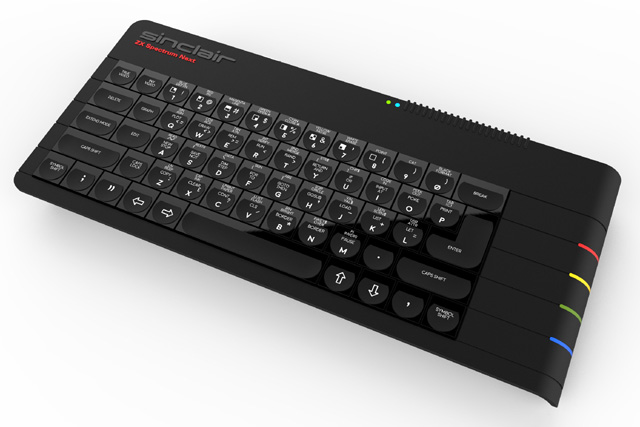
\includegraphics[width=.3\linewidth]{pics/spectrum_next} 
\end{center} 
\caption{ZX Spectrum Next, intended to be a fully functional iteration of the Sinclair ZX Spectrum. The makers claim it will be fully compatible with all software written for the original Spectrum \\ \textit{\small{Picture from \url {https://www.specnext.com/about/}}}}
\label{Spectrum_Next}
\end{figure} 

\textbf{Process}\\
The ZX Spectrum Next is an innovation of the ZX Spectrum from 1982. It is currently in the production phase of development after successfully raising \pounds 723,390 on a crowd-funding campaign on Kickstarter. When the crowd-funding campaign was launched on April 23rd 2017, the Next team had a working prototype with most of the hardware design finished, they did add some features later when the crowd-funding campaign was so successful 
\cite{RN151}. They also had CAD designs for the case and keyboard completed before the campaign 
\cite{RN149}. With the capital raised from the crowd-funding campaign they intend to fund the first production run of the Spectrum Next. Not long after the end of the campaign which was on the 23rd of May 2017, The Next team released a website to act as a Next portal to house information for the community including hardware, software, drivers and firmware for the Next 
\cite{RN154}. In April 2018, the Next team promised to have fortnightly updates on the Kickstarter page, this was in response to backers requests 
\cite{RN155}. They also mentioned they have nearly decided on a manufacturer for the keyboard and the case 
\cite{RN155}. The electronic manufacturer had been decided earlier 
\cite{RN151}. The Next team also mentioned in April 2018, their plans for the box and manual that would be included with the Next 
\cite{RN151}.\\

\textbf{Steps Identified}
\begin{enumerate}
\item Construct a working prototype without case or keyboard. 
\item Create finished CAD drawings of the keyboard and case.
\item Launch crowd-funding campaign to raise funds for the first production run.
\item Refine prototype to add new features, made possible by the crowd-funding campaign raising more than expected. 
\item Regularly make updates to backers informing them of the progress made or problems faced.
\item Launch website portal to house community information and have online presence outside of Kickstarter.
\item Decide on manufacturers or keyboard, case and electronics.
\item Have manufacturers produce sample products for testing and quality control.
\item Adjust CAD drawing and make any other changes needed based on samples from manufactures.
\item Secure components for manufacturing e.g. RAM, resistors, capacitors etc. 
\item Finish work on manual and box designs and content.
\item Agree to start final production run with manufacturers. 
\end{enumerate} 

\textbf{Challenges faced during productisation}\\
The makers have had trouble with the mechanical function of the keyboard which has delayed production while they try to fix the issue. The last given expected delivery date was the 2nd quarter of 2019. There is also evidence the firmware the Next is running is still under development. The Next team also mentions problems with the exchange rate, as the value of the pound had been falling compared to the US dollar during the production period, this made it hard for them to source all the components within their budget 
\cite{RN159}. The Spectrum Next team also had to consider the effects of Brexit 
\cite{RN157}. The chosen manufacturer of the case unexpectedly left the project due to the then manager resigning, and the new manager not considering the project worthwhile for their business 
\cite{RN158}. This caused some delay as the team had to find a new case manufacturer, the Next team was also worried about incurring storage costs because of this. If the keyboards were finished before the case then they would have to go into storage, costing the Next team extra money. It turned out that due to delays with the keyboard, this wasn't an issue. Another issue faced was due to a stretch goal (a stretch goal is an additional goal for the crowd-funding campaign that was above the first goal of funding the production), the inclusion of RAM sockets that would allow new RAM to be added without the need to solder, caused some problems as the devices are not in common usage any more and thus hard to buy or get manufactured. They did eventually find a manufacturer which still had the parts to make the sockets and that also agreed to make a small run for the Next 
\cite{RN159}. \\

\textbf{Relevant useful lessons gleamed from the study}
\begin{enumerate}
\item The time taken for quality control and testing of moving parts, such as buttons and keys, can escalate and endanger the entire project.\\
\end{enumerate}

\textbf{Challenges}
\begin{enumerate}
\item Keyboard mechanism design issues
\item Crowd-funding in currency other than US dollars made it difficult to source components
\item Brexit
\item Supplier failure to deliver
\item Sourcing old component 
\end{enumerate}

%%%%%%%%%%%%%%%%%%%%%%%%%%%%%%%%%%%%%%%%%%%%%%%%%%%%%%%%%%%%%%%%%%%%%%%%%%%%%%%%%%%%%%%%%%%
\subsection{C64 Mini}
\textbf{What is it?}\\
A mini form factor game console inspired by the Commodore 64. It also is a fully functional Commodore 64-like computer which can be control via a USB connected keyboard (not included). It has a non-functional keyboard and a functional joystick which connects to the console via a cable. The console connects to a TV to display in 720p resolution. The C64 Mini came pre-loaded with 64 game written for the Commodore 64, it also has the ability to load game ROMs from a USB flash stick. It was funded through a crowd-funding campaign on Indiegogo 
\cite{RN124}, the campaign was intended to raise funds to pay design work on the case and keyboard as well as pay for the first production run. The creators of the Mini are Retro Games, they originally planned on releasing a full-size and hand-held console (with build-in screen) form factor but during the production period, on the 28th of April 2017, they pivoted to focus on the C64 Mini form-factor with the full-size version to follow later 
\cite{RN160}. It's interesting to note that the resigned directors of Retro Computers (the company behind the unpopular Vega Plus campaign), Paul Andrews and Chris Smith (they resigned before the company went off the rails) are involved, as well as Darren Melbourne who worked on the C64 DTV 
\cite{RN127}. The Mini has a ARM SoC at its core, which runs a software emulation of the C64 
\cite{RN160}. Retro Games have stated that they will open-source the designs as much as possible once the production is complete, currentley they have not even though the C64 Mini has been released but the full-size version is still under production\\

\textbf{When was it produced?}\\
Released in the first quarter of 2018. \\

\textbf{Why was it produced?}\\
A commercial endeavour. \\

\begin{figure} \begin{center}
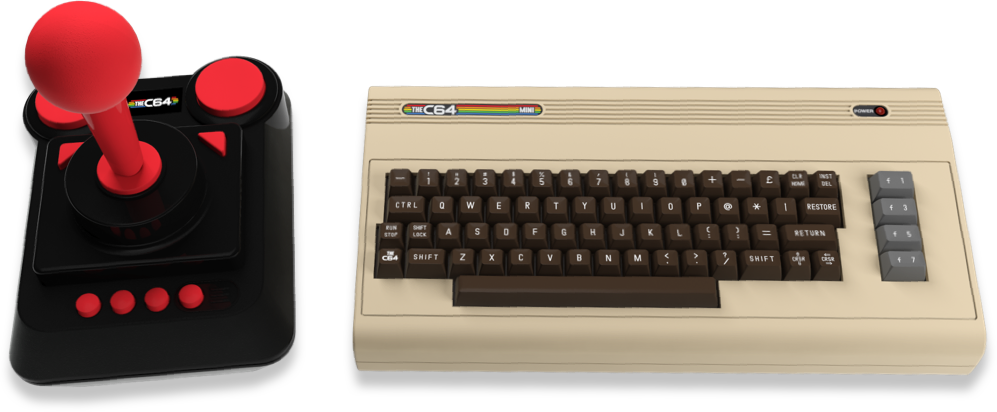
\includegraphics[width=.3\linewidth]{pics/C64_mini} 
\end{center} 
\caption{C64 mini\\ \textit{\small{Picture from \url {https://retrogames.biz/thec64-mini/}}}}
\label{C64_mini}
\end{figure}

\textbf{Process}\\
Retro Games didn't have a functional prototype at the campaign launch, it wasn't shown till August 2016, running on preproduction hardware. After campaign had finished, Retro Games tried to partner with a manufacturer and distributor to get the c64 worldwide retail release. Retro Games secured extra funds missing from crowd-funding campaign as well as focusing on c64 Mini first at partners request. Retro Games worked on circuit design for 3 form-factors of the C64 range, as well as CAD designs for case and keyboard and component selection. Retro Games also sought agreements from game developers to use their games in the Mini during production period. \\

\textbf{Steps Identified}
\begin{enumerate}
\item Launch crowdfunding campaign.
\item Create functional prototype on preproduction hardware.
\item Find partner to invest, manufacture and distribute.
\item Re-evaluate with partner best business direction (Retro Games focused on C64 Mini form-factor)
\item Secure game rights.
\item Finish circuit designs for final product and component selection and sourcing. Design with compliance in mind.
\item Create CAD drawings of case and keyboard.
\item Create manual and box design.
\item Test pre-production units and make amendments to product or processes as needed.
\item Start production run and send to backers.
\item Retail release.
\end{enumerate} 

\textbf{Challenges faced during productisation}\\
The crowd funding campaign did not meet the target goal of \$150,00 USD, reaching 67\% of the target or \$100,611 USD. Retro Games delayed their production schedule because of this, but ultimately they reached an agreement with an international distributor and manufacturer which allowed them to continue without seeking further funding
\cite{RN125}. This collaboration with the aforementioned partner also lead Retro Games to rethink their plans, they pivoted to focus on the C64 mini version entirely and get that complete first before moving to the full size version. \\

\textbf{Relevant useful lessons gleamed from the study}\\
Regular communication with backers is important for a successful crowd-funding campaign, this includes listening to them and responding to their concerns and queries. Paul Andrews and Chris Smith must have been aware there could be potential backlash over their involvement in the Vega Plus quagmire (they were both directors of Retro Computers when the Vega Plus campaign was launch but left a few months later). They remained honest (to the best of my knowledge) about the situation and who they were and probably of most importance, gave regular weekly updates to backers describing progress made and relevant news as well as progress pictures whenever possible. They also, on several occasions, publicly answered specific questions from backers, which would go a long way to alleviating fears and concerns from the backers about a repeat of the Vega Plus campaign.  \\

\textbf{Challenges}
\begin{enumerate}
\item Failure to reach crowd-funding goal
\end{enumerate}


%%%%%%%%%%%%%%%%%%%%%%%%%%%%%%%%%%%%%%%%%%%%%%%%%%%%%%%%%%%%%%%%%%%%%%%%%%%%%%%%%%%%%%%%%%%
\subsection{C64 DTV}
\textbf{What is it?}\\
A single-board Commodore 64 clone housed within a joystick, comes preloaded with 30 games. It was, unsurprisingly from the name, inspired by the Commodore 64. It features an ASIC (Application-specific Integrated Circuit) at its core 
\cite{RN129} and has the possibility of after market modification due to exposed solder points on the board
\cite{RN126}. The C64 DTV was born from another project, the C-One which was also created by the DTV's designer, Jeri Ellsworth. The C-One is a single-board C64 clone made using FPGA technology.\\

\textbf{When was it produced?}\\
First released in 2004 with version 1, which support only NTSC Broadcasting Television standard. Version 2 came out in 2005 with additional PAL support\\

\textbf{Why was it produced?}\\
A commercial endeavour. \\

\begin{figure} \begin{center}
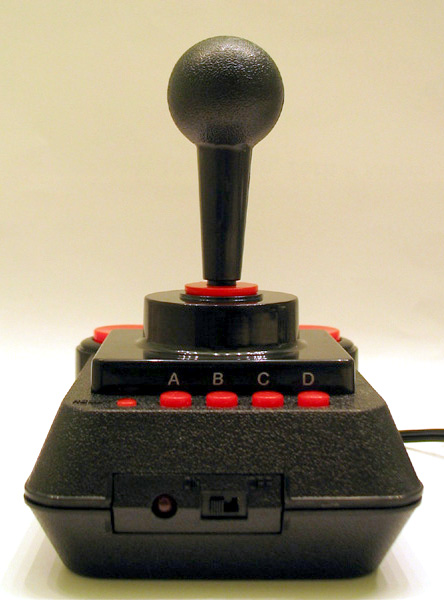
\includegraphics[width=.3\linewidth]{pics/C64_DTV} 
\end{center} 
\caption{C64 DTV or C64 Direct-to-Television \\ \textit{\small{Picture courtesy of Christian Wirth}}}
\label{C64_DTV}
\end{figure}

\textbf{Process}\\
The C64 DTV was an innovation of an earlier product, the C-One. The C-One is a single-board C64 clone that uses FPGA technology. The DTV is a smaller version of the C-One which fits into a accompanying joystick case, as shown in Figure \ref{C64_DTV}. The DTV is aimed at letting users play Commodore 64 games, of which 30 were included. The DTV does not support the ability to load game ROMs after purchase but it is possible with some after-market modifications 
\cite{RN161}.\\

\textbf{Steps Identified}\\
\begin{enumerate}
\item Construct a working prototype to fulfil an idea or need, the prototype here is taken as being the prototype which lead to the C-One. 
\item Partner with others that can help turn the prototype into a product, the C-One.
\item partner with others that have skills to develop a games console based off the C-One.
\item Design and create the C64 DTV case including joystick and PCB based off the C-One.
\item Form partnership to market and distribute product.
\end{enumerate} 

\textbf{Challenges faced during productisation}\\
The C64 DTV was derived from another similar product, the C-One. Jeri Ellsworth designed an enhanced version of the Commodore 64 as a way to teach herself about programming FPGAs. Ellsworth then partnered with Individual Computers to turn her FPGA design into a product, the C-One. Other manufactures and retailers saw potential in the C-One and asked Ellsworth if she would consider making a smaller version that would fit in a joystick, with a focus on enabling users to play games, shown in Figure \ref{C64_DTV}. Unfortunately it seems very little was published about the process from turning the C-One into the C64 DTV or from earlier efforts to complete the C-One.\\

\textbf{Relevant useful lessons gleamed from the study}\\
\begin{enumerate}
\item Retro games can sell quite well, nostalgia is a powerful incentive.
\item Extra features included in the device can help boost sales, these can be features that are not normally available but the device can be hacked or modified by the user to make them available. There are reports of user buying the DTV simply to access the C64-like computer running at its core.
\item ASICs are a technology that could be applied to this area.
\item There is a larger market for consoles that focus on playing games than other uses of a 8-bit computer.
\end{enumerate}

\textbf{Challenges}
\begin{enumerate}
\item None identified
\end{enumerate}

%------------------------------------------------------------------
%------------------------------------------------------------------
\section{Retro-computing productization: process}
\label{sec: Retro-computing process}
This section consolidates the processes collected from the case studies above. A discussion of any interesting or useful conclusions drawn from the comparison follows.\\

\subsection{Combined process from case studies}
The following is a combination of the processes identified in the case studies. The steps that are common to all or most case studies are included, as well as two possible funding models.\\

\textbf{Combined Process}
\begin{enumerate}
\item Construct a working prototype.
\item Control IP.
\item Research relevant laws and regulatory obligations and make design changes to accommodate as well as budgeting for any costs likely to be incurred in future testing.
\item Decide final product features and specifications based on prototype feedback.
\item Add team members as needed to help grow the project. Focus on what skills they can provide when deciding on members.
\item Create CAD designs for case, keyboard and any other parts that need to be custom made for the final product.
\item Launch crowd-funding campaign or raise funds through private investors or businesses for first production run.
\item Refine prototype to remove bugs/errors and add any features that are required for the product launch.
\item Launch website to give a web presence and foster a community.
\item Find manufacturer for electronics, plastics (case, keyboard etc.) and source components.
\item Partner with or form agreements with distributors to increase the availability of the product and market the product.
\end{enumerate} 

Most of the discovered processes from the case studies agreed on an outline of a process to productization, which is listed above. One of the points of difference between the processes identified in the individual case studies is how much of the design work was complete before announcing the release of the product to the public, either through a crowd-funding campaign or other method. The decision to announce earlier in the design process may be due to businesses constraints, if the project is in need of funds to continue, then announcing early may be worth the increased risk. The risk in announcing early is due to uncertainty in several factors: currency changes, law changes such as 'Brexit', unknown costs for manufacturing and design changes. The other main point of difference was to use a crowd-funding service to raise capital or to rely of private investor and/or business partnerships or a mixture of both. With regard to a crowd-funding campaign, it has been proven to be possible to be successful but a successful campaign, such as the Next, Vega and Vega+ had several common features. Successful in this context relates solely to the campaign's fund raising effort, not the end result generated from the funds. The 3 campaigns named, all had a lot of information about the product as well as a working prototype to show in video. All 3 campaigns also posted regular updates as well as responding to community requests and/or concerns.

It is hoped that the process described here will be useful for new retro computing projects and form a basis for further research in this area. \\

\begin{figure} \begin{center}
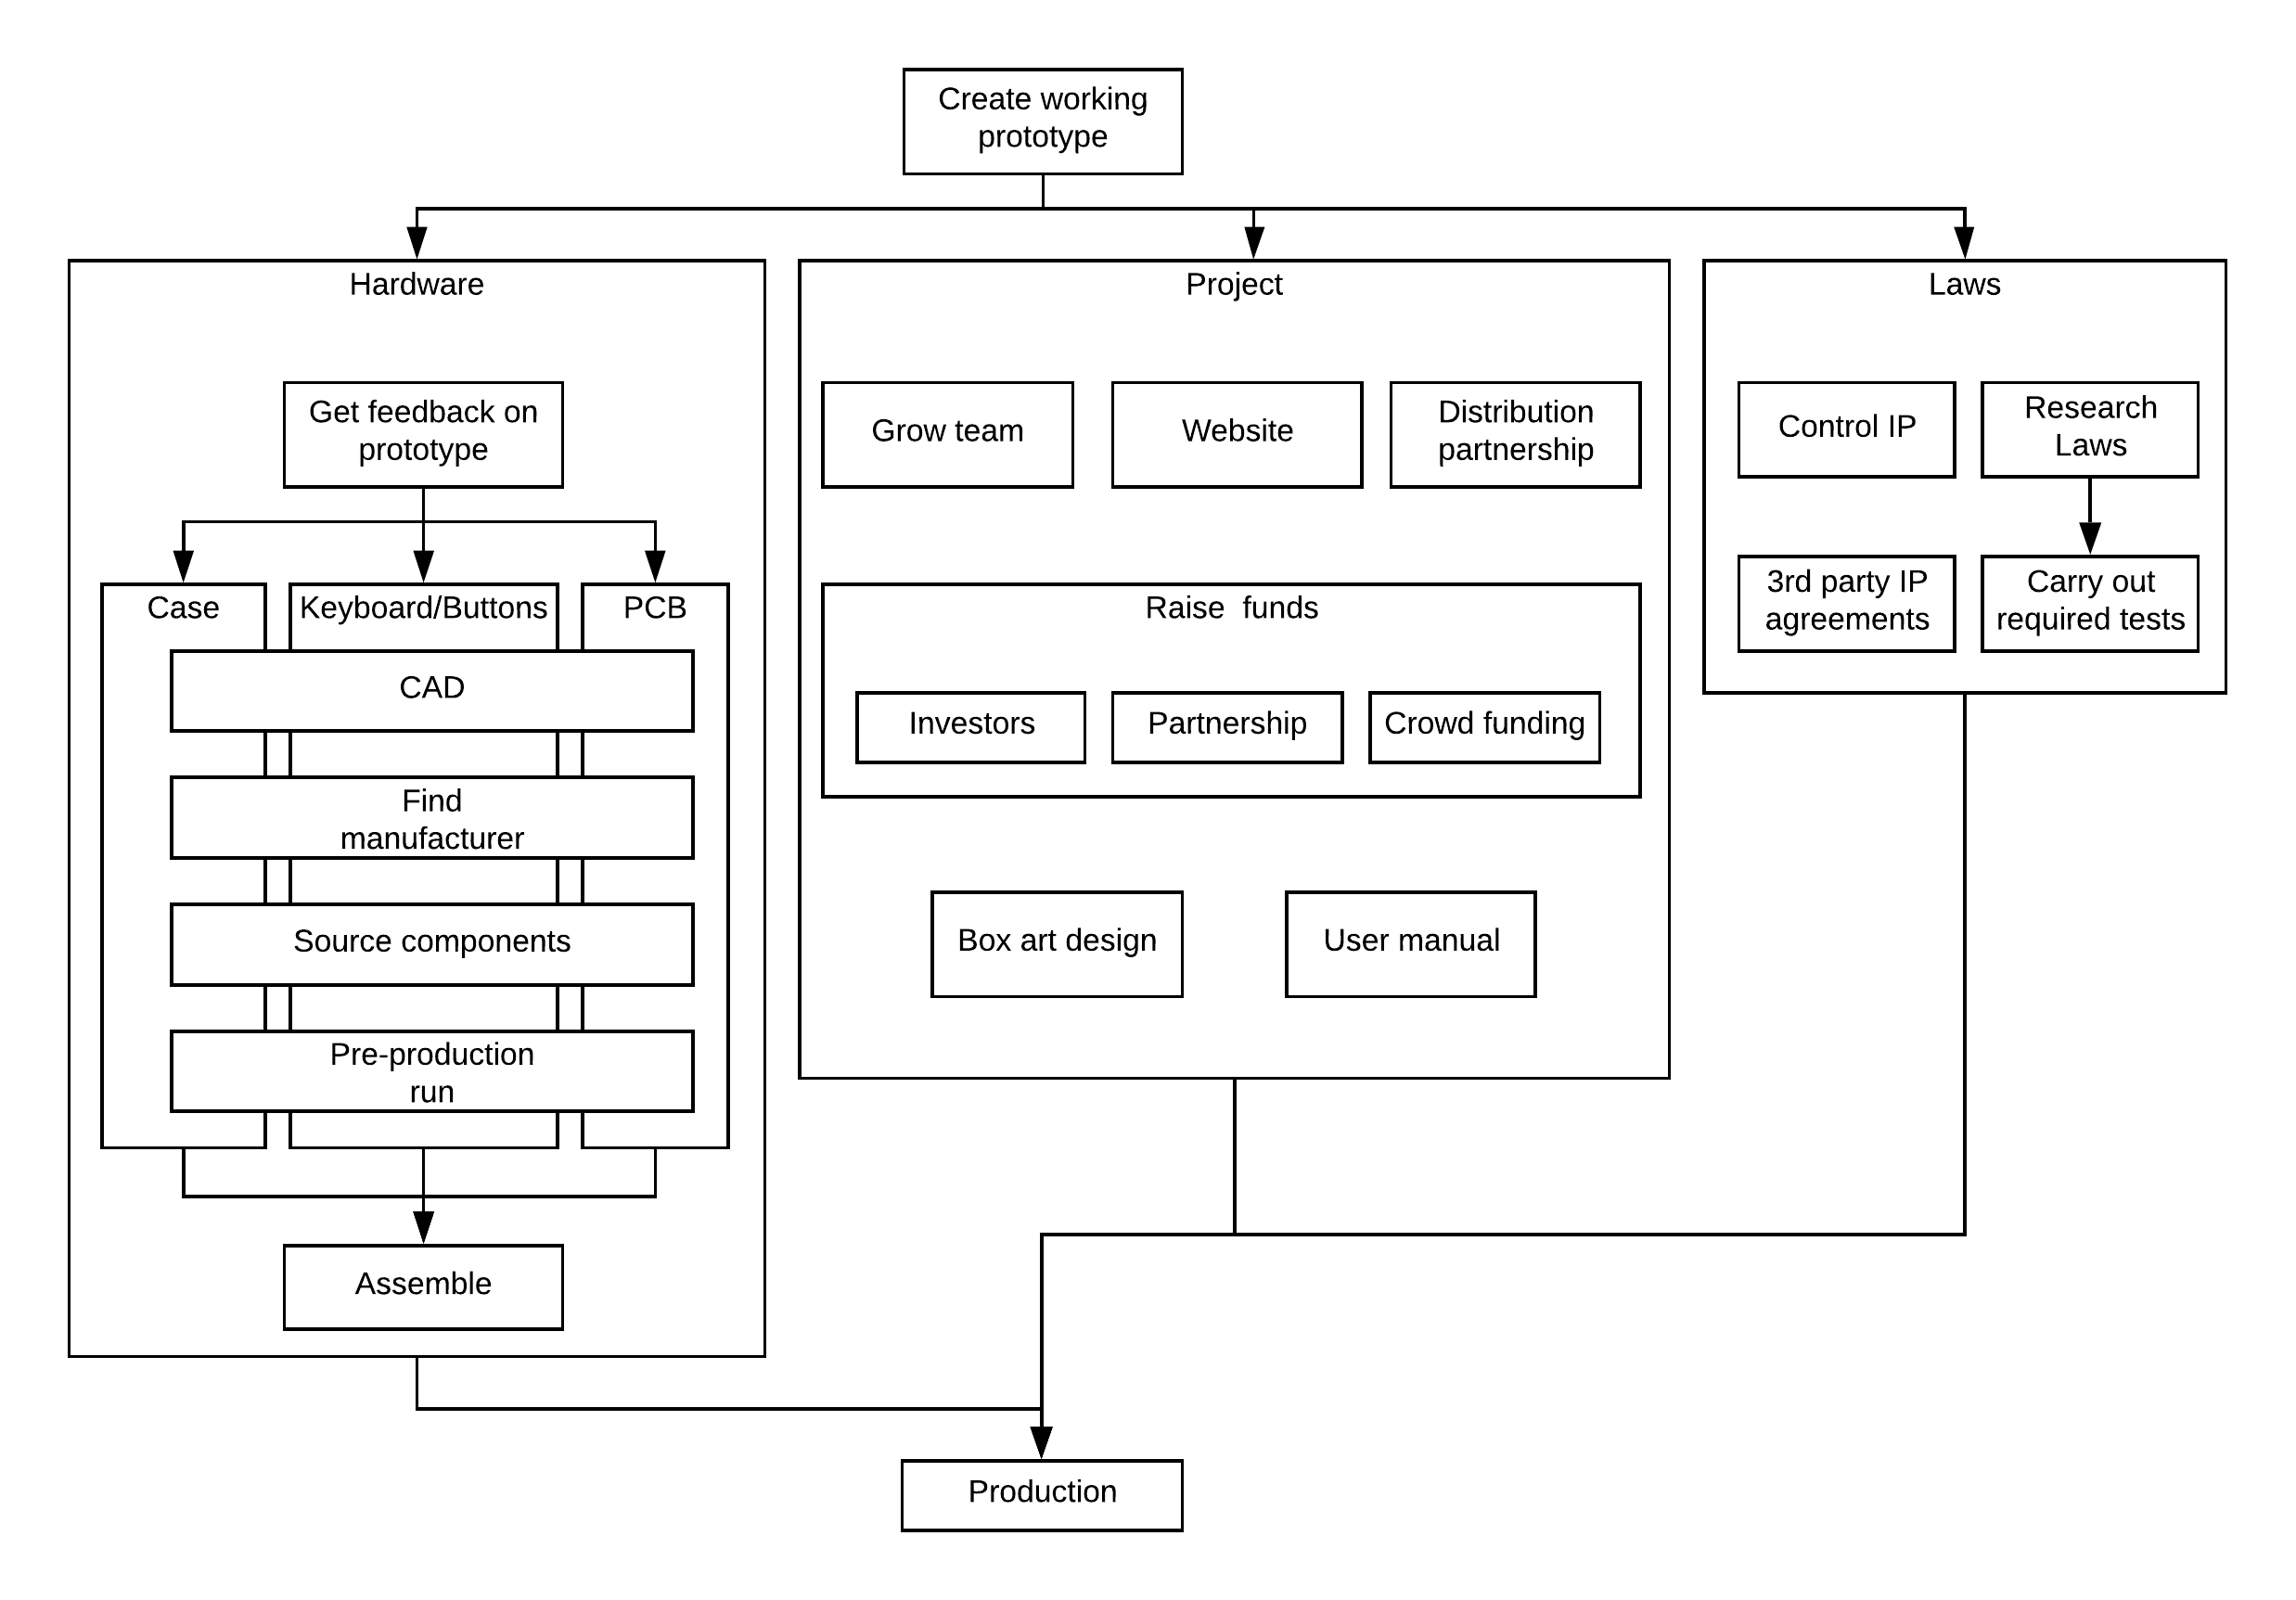
\includegraphics[width= 1\linewidth]{pics/case_study_process} 
\end{center} 
\caption{Retro-computer productization process. Small rectangles are tasks, larger rectangles are task areas.}
\label{case_study_process}
\end{figure} 

%------------------------------------------------------------------
%------------------------------------------------------------------
\section{Retro-computing productization: associated risks}
\label{sec: Retro-computing risks}
The challenges identified in the case studies are categorised into risks and ranked to produce a list of risks that are relevant to retro-computer projects. It is intended these risks be considered along side the typical project risks, which have been well researched and documented in previous research efforts. 

For each identified risk, the challenges within the case studies which fit within the risk category are mentioned. A description of the risk is given, and the factors which affect its potential damage and likelihood of occurring are also discussed.

The risks are ranked by their worst-case potential damage to the project and are shown in figure \ref{risk list}. The ranking is based off the following definitions:
\begin{enumerate}
\item Negligible 	- Slight time delay or cost on project.
\item Marginal 		- Moderate time delay or cost on project. 
\item Critical 		- Extensive time delay or cost to project.
\item Catastrophic 	- Project cannot proceed.
\end{enumerate}

\subsection{Laws and regulations}
This risk category is related to the laws and regulations of specific markets within which a retro-computing project wants to operate and sell products. The potential damage from this risk comes from the delays and additional costs that complying with these laws and regulations may attract. This could be due to a project not being aware of required testing and as such not planning and conducting the required tests in a timely manner. Additionally, there could be further costs and delays if the product fails aforementioned tests and requires changes to the product in order to pass the test or tests. The worst-case scenario would involve the product failing a required test and the product being unable to be changed to pass. 

Several case studies ran into problems complying with the required laws or regulations specific to the markets they wanted to enter. The Raspberry Pi experienced some delays because the team didn't think their product needed to undergo electronic emissions testing when in fact it did. By the time the team realised this was the case, it was too late to avoid any delay and still undergo the testing. The C64 Mini project also experienced a delay due to age-rating testing and certification.  

A factors which affects the potential damage caused by this risk is how far along the productization process the project has progressed before the project becomes aware of all the required laws and regulations which they must abide by. If a product is practically complete and ready for release on the market, then any changes could be catastrophic. Inversely, if a product is still in the design phase when the required laws and regulations are researched, then any changes may be easily undertaken with minimal cost.

\subsection{Brexit-like event}
Brexit is the unofficial name given to the event of the United Kingdom leaving the European Union. This is a very specific event and will not need to be considered soon, as Brexit will have been finished. The Brexit-like event is used here to illustrate the type of large policy changes that can affect retro-computing projects if their customers, partners or their team is situated in a country undergoing an event such as Brexit. Large scale trade wars and economic recessions are other similar large scale events that should be considered. 

In the case of Brexit, it is causing some concern for the Next team that a post-Brexit environment may have unforeseen laws and regulations they need to abide by to sell in European countries. 

The factors which affect the likelihood of a Brexit-like event are too numerous to be discussed here in full, but the global political landscape and volatility in markets such as the share market can be useful indicators. One factor which affects the potential damage is the geographic region in which the event is occurring and if the retro-computing project in question is located in or intends to sell into that region.

\subsection{Crowd-funding}
There were several challenges associated with crowd-funding which were highlighted during the case studies. The specific areas are covered in depth below. 

\subsection{Crowd-funding: Contract of sale}
This risk is associated with any retro-computing project that uses crowd-funding to generate funds. The risk comes from the potential for backers of the campaign starting legal proceedings against the campaign founders. These legal preceding are spurred by backers not receiving what they believe they are entitled to, namely the product offered to backers of the campaigns. This could be because the product was never delivered, delivered late or there were significant changes to the product. The most visible example of this risk came from the case study of the Vega Plus project.  

A factor which affects the potential damage caused by this risk is the amount and value of the items promised to backers of a crowd-funding campaign. If the backers are promised several relatively expensive products for backing then the potential damage is greater as each backers may bring a lawsuit seeking higher damages than if the promised products were less valuable. 

The likelihood is increased by several factors, the amount and quality of the interactions between the campaign founders and the backers is one of them. If the campaign founders, the retro-computing project in this case, regularly post updates on the progress that is being made and interact honestly and are upfront about any problems, then the likelihood is reduced. If on the other hand the founders do not interact with the backers or repeatedly make promises which they do not keep, then the likelihood is increased.

This risk was given a catastrophic rating as the legal problems resulting from this event occurring could have stopped any of the crowd-funded projects in the case studies from being complete. Although it is arguable that they got to the state where backers were successfully suing the campaign founders, then there's a good chance the project was already in trouble.\\

\subsection{Crowd-funding: Currency}
This risk is associated with the choice of currency chosen for a crowd-funding campaign. A crowd-funding campaign is normally set to a specific currency at the beginning, the risk comes from the chosen currency losing value in the time period before it's to be spent. The Spectrum Next case study uncovered this risk. 

A factor which increases the likelihood of this occurring is the choice of currency, certain currencies are historically more stable. Retro-computing projects conducting research into recent currency trends before making a decision on currency, could reduce the likelihood of this even occurring. The markets and their respective currencies in which the funds are to be spent is another factor.

The potential damage is increased with time, the longer between the receiving and the spending of the funds increases the damage as the value of the currency has more time to change. 

\subsection{Crowd-funding: Failure to meet fund-raising goal}
This risk is describing the event of a retro-computing project running a crowd-funding campaign to completion, but not reaching their pre-determined funding goal. This can lead to a retro-computing project not having the required funds to continue. This risk was highlighted by the C64 Mini case study.

A factor which affects the likelihood of this event occurring is the quality, amount and trustworthiness of the media content used describing the retro-computing project. If potential backers decide that the retro-computing project has a high chance of success, then they are more likely to fund the campaign. To make this decision they would normally rely on the videos, written descriptions and other content the crowd-funding campaign founders would produce. Other factors include how much attention and media coverage the campaign receives, and how big of a market there is for the new product. 

The potential damage caused by this risk is affected by the retro-computing projects funding model. If the project has the ability to generate funds from private investors or it can form a partnership with another business which can provide the funds, then the damage can be negligible. If the retro-computing project has no other way to fund its endeavours, then the harm can be catastrophic. 


\subsection{Sourcing old components}
The use of old components can bring increased risk due to lack of supplies, manufacturing techniques or tools required to produce them. Old components is taken to mean components that are no longer frequently used to build modern electronic devices. Some retro-computing projects like to incorporate old components because those components were used on the computers which inspired them. The Spectrum Next experienced this problem, it's inspiration, the ZX Spectrum used ICs connected via sockets for RAM. This allowed the RAM to be changed without the use of tools. 

Factor which affect the likelihood of this risk occurring are the components frequency of use in production, availability of supplies, amount being produced currently among others. The general rule being that the rarer a component is, the more it will cost to purchase or manufacture. As time goes by, the likelihood will increase for any particular component, this is due to components being made redundant as new designs emerge.

The potential damage is increase for retro-computing project in which the aforementioned component is critical to the product. If the component cannot be replaced with an alternative as it would stop the retro-computing project of reaching their goal of recreating or innovating a home computer, then the damage can be catastrophic. Alternatively, if the component forms parts of a feature which is not critical, then potential damage may be negligible as the feature could possible be removed without stopping the project reaching their goal.


\subsection{Use of 3rd party intellectual property}
This risk is associated with the use of 3rd party intellectual property (IP) and the potential for the rights holders to undertake legal challenges against that use. All of the retro-computing projects from the case studies used or attempted to use 3rd party games with their software. Every project studied handled this very well, except for one stand-out failure, the Spectrum Vega Plus. 

The likelihood of this event occurring is affected by the rights holders attitude towards the use of their intellectual property. Retro-computing projects may find investigating recent legal challenges and how other projects have used the specific intellectual property beneficial. Some intellectual property used in previous retro-computing projects and home computer era computers, have ambiguous owners or have been regularly shared without challenge from the owners. This can make obtaining an agreement with the owners impossible or potentially unnecessary, but doesn't reduce the likelihood of the risk occurring. An agreement with the right holders will dramatical reduce this risk. The amount of IP also affects the likelihood, the more rights holders which are affected, the higher the chance of this event occurring. The popularity and potential profit a retro-computing project generates is also a contributing factor, if a project is hugely successful and profitable then it is more likely the right holders mount legal challenges.

The potential damage is affected by the features of the retro-computing product that are reliant on the 3rd party IP. If the IP is used as a critical component of the product, then the damage from its forced removal could be catastrophic. If the IP is a minor feature or a component which can be replaced with a similar component, then the damage is reduced.


\subsection{Open-source business}
This risk is caused by a project trying to be both open-source and profitable, the open-source nature of the designs can make it easier for competition to enter the market. The Arduino project gave insight into how an open-source business can be successful. If a project changes the way income is generated, as the product grows in popularity, it be profitable. In the beginning of a products life-cycle an open-source project can generate income in much the same way as a more traditional proprietary-based technology business. By being the first to market an open-source project can beat any production competition and generate an income. Over time, if the product is popular enough, competitors may enter the market and use the open-source designs to manufacture their own products and reduce the possible income for the original project. By being ready to respond to this possibility by altering the business model and focussing more on accessories for the product, commissioned constancy work or speaking at presentations as examples, the retro-computing project can still make a profit.

The likelihood for this occurring is affected by the amount of designs from within a retro-computing project are open-source. If everything is open-source, the likelihood is increased due to the lessened cost to a competitor trying to produce the product. The likelihood is also increased if the retro-computing product produced is popular. The more popular it is, the more potential for profit a competing manufacturer could generate.

The potential damage is affected by the structure of the retro-computing project's team and its ability to adapt to changes. If a retro-computing project team is too entrenched around generating profit from selling an open-source product and to slow to change when competition emerges, then the damage can be catastrophic.  


\subsection{Loss of use of intellectual property}
This risk is describing the event of intellectual property (IP) being withdrawn from use by its owners. This IP could have been created by team members of the project whom have changed there mind on allowing its use, or from 3rd parties how have given their agreement to use the IP but then have withdrawn it. The damage is caused by the legal challenges which can stem from the continued use of the IP, from the losses incurred in removing any IP from memory, documentation or marketing. This risk is most obvious from the Vega Plus case study, in which the CTO left with their design of the prototype shown in the crowd-funding videos. The Arduino case study highlighted a case where the Arduino team had to endure legal challenges against the use of the Arduino trade mark. 

This risk is dependant on the amount of IP used in the project and more importantly who holds ownership or who has agreement to use aforementioned IP. If the IP holder is an individual and their is no agreement in place to use the IP, or if the agreement allows the withdrawal of aforementioned IP without good reason, then the risk is increased. Inversely, if an entity associated with the project, such as the Raspberry Pi foundation, is the entity which holds ownership of the IP, then the risk is significantly reduced. An open-source ethos would also reduce the likelihood significantly as an open-source design is not possible to withdraw the right to use it. \\

\subsection{Supplier failure}
This risk describes the event of a supplier with which a retro-computing project has formed an agreement, not supplying what was agreed, either by being late, the supplied goods being wrong in some regard or the supplier being unable to provide any goods. This risk is not unique to retro-computing projects but is included because a case study into the Spectrum Next showed they experienced a delay when a manufacturer suddenly decided to not produce their product.

The potential damage and likelihood of this event occurring is specific to each supplier and each purchase. The likelihood of this event occurring can be reduced by using reputable, established suppliers as well as undertaking due diligence into suppliers before entering into agreements. The potential damage occurred is dependant on the nature of the purchase which the supplier failed to deliver as well as the nature of the failure. If the purchase was of a high critical component that the project needs to move forward, then the potential damage can be critical. If the purchase was for an incidentals part which could be easily obtained from numerous suppliers then the potential cost would be negligible.\\


\subsection{Open-source fair use}
This risk is associated with the use of open-source work and the potential for damage to reputation from the way in which the open-source work is used and the treatment of the open-source works creator(s). The Arduino project experienced a slight challenge from certain individuals that considered the way in which Banzi used the open-source work that formed the start of the Arduino project, as unethical. This mainly stems from the fact that Banzi was the supervisor of a student's project that Arduino was started from. Individuals expressed that they felt it was unethical to use the work without inviting the student in question to join the Arduino team.  

The likelihood is affected by the amount of open-source work from creators outside of the retro-computing project that is used within the project. More open-source work increase the likelihood. Another factor is relationship between creator and the retro-computing project, the closer the relationship the higher the likelihood.

The potential damage is relatively small for this risk, compared to the others, as it only has to do with loss of reputation and community backlash which may affect sales of a retro-computing project products but will likely not stop a project completely.  \\

\subsection{Physical production problems}
This risk is to do with the problems that can occurring during the design, manufacture or construction of a retro-computing product and the additional costs they can cause. As new components are manufactured and tested, problems can be highlighted which need to be addressed before the product can be sold. These problems can cause delays and incur extra costs to a project. The Spectrum Next experienced a delay due to the mechanism of the keyboard buttons. The Spectrum Vega Plus had a problem with the design and construction of their buttons, causing delays. 

This likelihood of this event occurring is increased by the amount of physical components and buttons required for a product. Also the nature of the buttons or other HID component, if it is a more standard component, following common practises, it will be less likely to suffer this event.

The potential damage is critical and affected by factors such as the manufacturing process used, the cost of tools or moulds needed and the amount of HID components or other physical components are needed as well as their complexity.\\ 

\begin{figure} \begin{center}
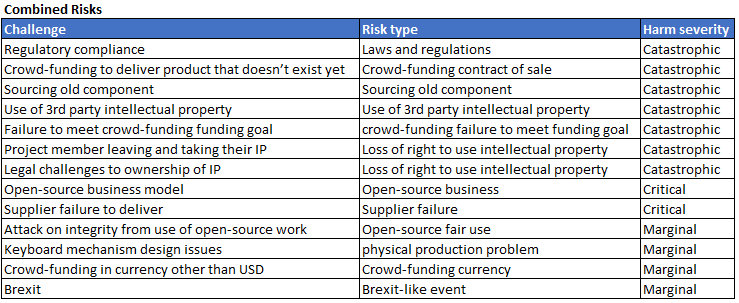
\includegraphics[width= 1\linewidth]{pics/risk_list} 
\end{center} 
\caption{Combined list of risk associated with a retro-computer project}
\label{risk list}
\end{figure} 

%%Chapter 4 - MEGA65: A retro revival project
%What does the retro computer productization process look like?

\chapter{MEGA65: A retro revival project}
\label{Chapter4}

This chapter outlines the current state of a retro revival project, the MEGA65, mentioned in chapter \ref{Chapter2}. By first giving a description of the intended products of the project as the project members intend. Then a use case study of the MEGA65 is carried out to further describe the product, it's intended markets and to elicit requirements to realise the use cases. This detailed information about the MEGA65 project is then used in the next chapter, chapter \ref{Chapter5} to evaluate the project against the risk list that was obtained from the case studies in chapter \ref{Chapter3}.
%----------------------------------------------------------------------------------------
%----------------------------------------------------------------------------------------
\section{MEGA65}
The MEGA65 is a innovation of the Commodore 65 built using FPGA technology at its core, more details are given in section \ref{History of the MEGA65 project}. The MEGA65 is planned to have two separate form factors: a hand-held game console with 2 cellular modem sockets to allow for telephony, called MEGAphone and a desktop form-factor inspired by the look of the Commodore 64. During development of the MEGA65, the MEGA65 team got into discussions with the Museum of Electronic Games and Art (MEGA) and came to an agreement with MEGA that they will handle the physical development of the MEGA65 desktop version. Both form-factors are to have the same FPGA chip and FPGA implementation. This means they are the same computer at the core and can run the same software, in fact both form-factors are intended to ship with the same software, both custom software made specifically for the MEGA65 and 3rd party software. Both form-factors are collectively referred to as the MEGA65. The MEGAphone is to be developed further at Flinders University, with the original MEGA65 team members as well as involving students from the university. The desktop version is to have its physical development handled by MEGA. Physical development refers to the Printed Circuit Board (PCB) housing the FPGA and other components, the case and keyboard. 

\subsection{MEGA65 team}
- make up of team
- project funding
- 

\subsection{Hardware}
Desktop
- 3.5 " floppy drive
- keyboard, full size etc
- SD card

MEGAphone
- touch screen interface
- d-pad, buttons
- cellular modems sockets
- speakers
- battery

\subsection{Software}
The MEGA65 has had a range of custom software created for it, this section aims to list and describe that software. This will help further describe the MEGA65 as a product as well as give some explanation of the functions available to these pieces of software which will be helpful to carry out the use case studies.\\

\textbf{Kickstart - the Hypervisor}\\
Kickstart is the name of the hypervisor. It is unusual because it is also like a BIOS and boot-loader in a modern operating system, as well as a hypervisor. It was custom built for the MEGA65 and fits in 16 KB. On start up, the hypervisor loads the BASIC ROM, BASIC formed the entire operating system on the Commodore 64. Kickstart also handles kernel operations as such it handles all the freeze operations for the Freeze menu. The hypervisor also contains a few utilities housed within FPGA RAM, these can be run from the hypervisor by holding down the two Shift keys on reboot. One of these utilities is a config menu, which allows changing of certain settings. Another is the FDISK utility which can format a SD into the required MEGA65 format, ready for first use.\\

\textbf{The Freeze Menu}\\
The Freeze menu is a program which allows for a variety of useful features. It can be entered into from any program by holding down the Restore key for 1/2 a second. When run, the Freeze Menu stops the current process or freezes it, and saves the state of the computer. This allows programs to be saved and swapped with other programs, then swapped back to, resuming from the original point, this feature is common in modern computers but it wasn't available on the C64. The idea was to get some of the same functionality as a 'freeze cartridge', a popular type of device in the Home Computer era. Some of the features available from the Freeze Menu are:
\begin{enumerate}
\item Restore and return to program which was running when Freeze Menu was run, by pressing F3.
\item Task switching.
\item View, select and load from disk images stored on a SD card.
\item Toggle video mode between NTSC and PAL.
\item Change CPU frequency between pre-set values: 1 MHz (C64 speed), 2 MHz (C128 speed), 3.5 MHz (C65 speed), 40 MHz (MEGA65 speed).
\item Change state of machine such as change register values which store the current amount of lives in a video game. This allows 'freeze cartridge' like 'cheats' to be used.
\item Setting options to set protected ROM and to enable the cartridge port.
\item Allow inspection of memory and allows changes to it. Action replay-like freeze cartridges used features like this to modify games. This is functional but missing some features which are listed below.
\item Audio mixer. It is functional but very basic.
\end{enumerate}

\textbf{Matrix Mode}\\
An out-of-band machine state inspection tool which allows the user to inspect the RAM, ROM, and CPU, I/O registers.\\

\textbf{Secure Mode}\\
Is a special mode to allow the untrusted components of the MEGA65 to be excluded from the current working environment. This includes the cellular modem and SD card among others. Figure \ref{secure_compartment} shows the secure compartment and the untrustworthy components.\\


\begin{figure} \begin{center}
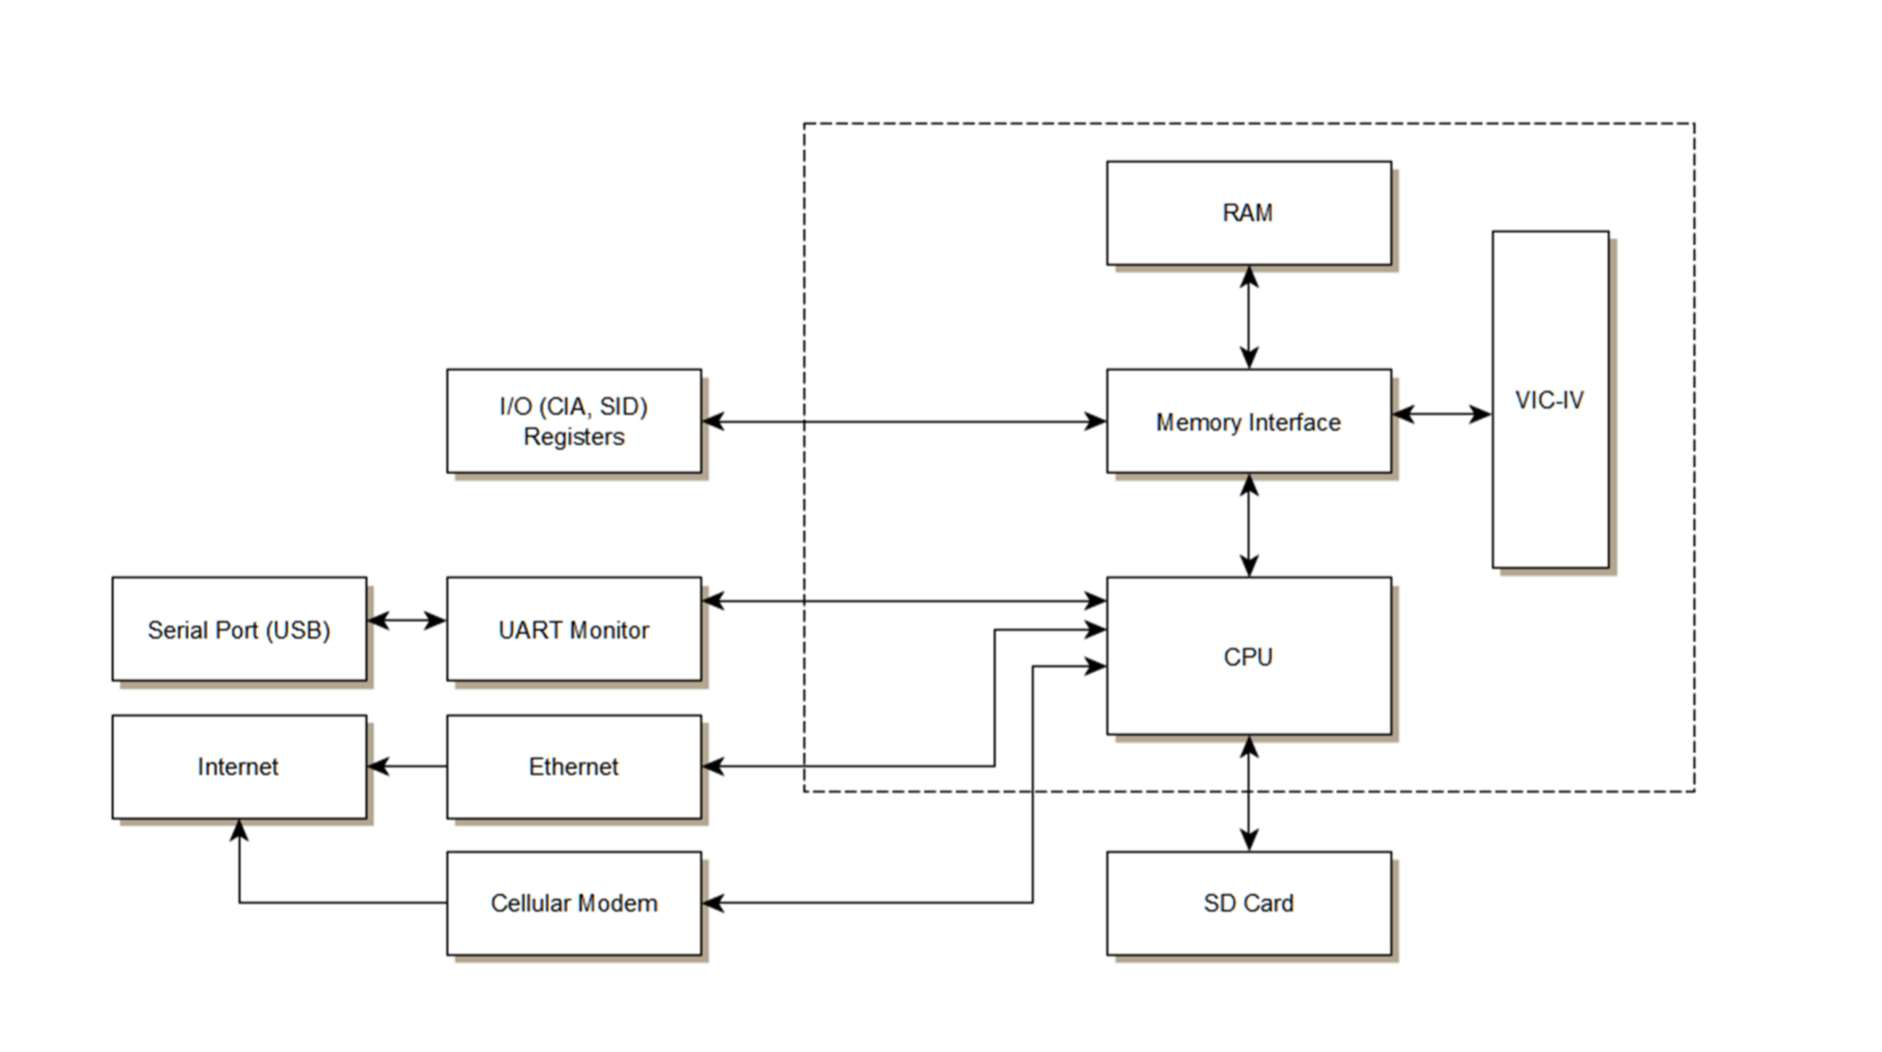
\includegraphics[width=.3\linewidth]{pics/secure_compartment} 
\end{center} 
\caption{Secure compartment of the MEGA65. All untrustworthy components are outside of the container.\\}
\label{secure_compartment}
\end{figure}

\textbf{Applications}\\
This section talks about the application that have been made by MEGA65 project members for the MEGA65. The current plan is for both form factors to be able to run the same software and include the same software on release. There should be no problem with taking the SD card from one machine and running it in the other, as an example.\\

\textbf{MegaWAT} \\
MegaWAT is an open-source slide presentation and editing application \cite{RN163}. It features:
\begin{enumerate}
\item Text editing with colours, attributes and typeface selection
\item Multiple slides
\item Presentation mode
\item Load and save
\item Changeable screen colour
\end{enumerate}

\textbf{MEGA65 IDE}\\
There is also a MEGA65 IDE, which currently only allows viewing of text files. It does currently support viewing of multiple files at once, up to 5 in separate windows, which it can be switched between and the files scrolled through.\\

\textbf{Telephony software}\\
This application allows phone calls to be made over a cellular modem, which the MEGAphone will have sockets to install two of them. \\


\section{Use case study}
This sections lists and discusses use cases for the MEGA65 in both its form-factors, the desktop computer and the hand-held console. It is hoped that by studying the way the MEGA65 might possibly be used and extracting the features required to fur fill each use case, that a clear description of the MEGA65 can be formed. The requirements can then be used to help capture the current state of the MEGA65 in terms of its development. This list can then help with decision making regarding the minimum viable product for the MEGA65, but that is outside the scope of this thesis. The use cases where first decided upon by determining some roles or actors from the MEGA65's target market, with help from MEGA65 team members. These actors are described below, as well as a brief look at there likely use cases as seen in figure \ref{MEGA65_use_cases}.

\subsection{Actors}
\textbf{Gamer}\\
The Gamer's goal is to be able to play retro games. The amount of games and the ability to add more games as well as controller options such as an external joystick are all important to this actor.\\

\textbf{8-bit Programmer}\\
The 8-bit Programmer referred to as just Programmer from here on, has a goal of being able to run 8-bit programs in a C64 or C65 environment. They are interested in any features which will add compatibility such as support for different opcodes or new video modes. \\

\textbf{Tech Enthusiast}\\
The Tech Enthusiast's goal is to try new technology and experience rare or peculiar technological devices, this group also contains 'modders' or 'hackers', people that like to change products they have been purchased. They are interested in any of the features but especially in the features that will add something unique or the ability to modify the product easily.\\

\textbf{Privacy Motivated}\\
The Privacy Motivated actor's goals is to be able to securely communicated and carry out a variety of tasks. They are interested in features that will let them thwart any malicious attempts to obtain data. Features that will allow the actor to perform check as increase trust of the security of the device will also be highly valued. \\

\textbf{Educator}\\
The Educator's goal is to teach computer skills and/or topics to others. They are interested in simple computer systems, as this will help highlight the fundamentals of a computer. They are interested in being able to easily write and run code. They are also interested in presenting slides and using 8-bit applications for teaching purposes.\\

\begin{figure} \begin{center}
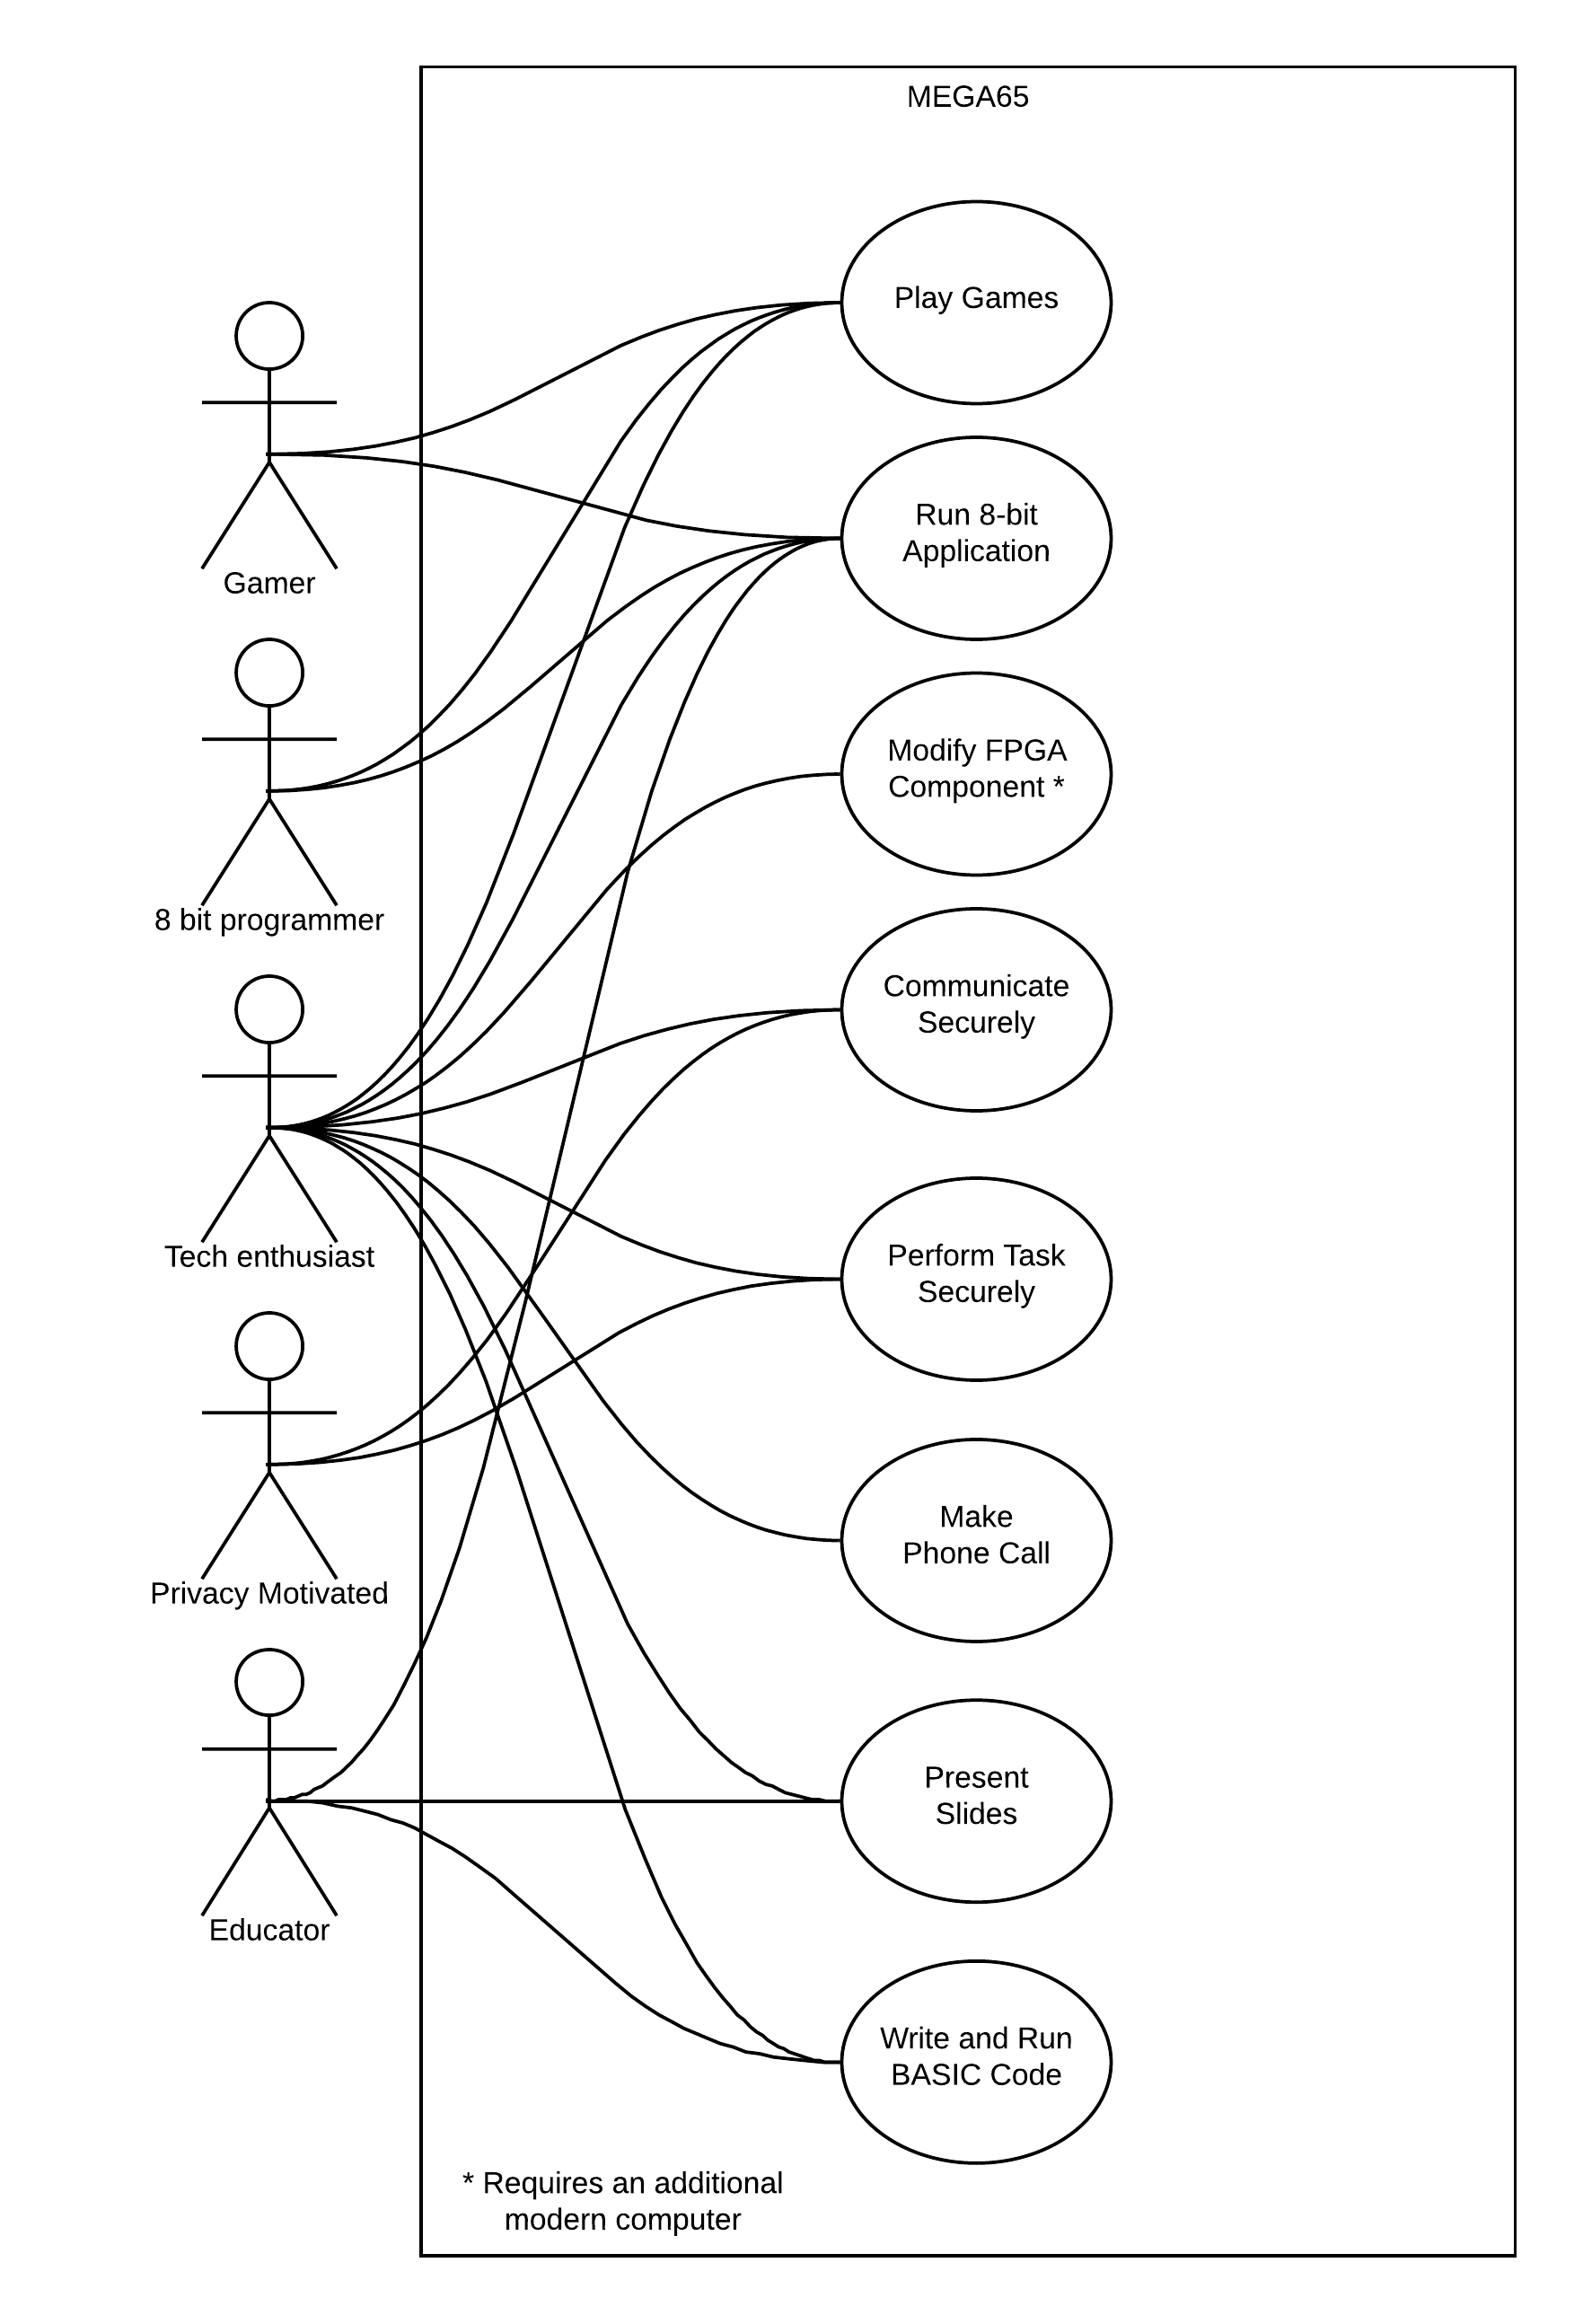
\includegraphics[width=.6\linewidth]{pics/MEGA65_use_case} 
\end{center} 
\caption{MEGA65 Use Cases for the target market\\}
\label{MEGA65_use_cases}
\end{figure}

\subsection{Use case narratives}
This section describes the use cases in a narrative form. The narrative tries to cover all the likely ways to interact with the MEGA65. Where the narrative is for a specific form-factor of the MEGA65 it will be stated, otherwise assume it is for both form factors. \\

%%%%%%%%%%%%%%%%%%%%%%%%%%%%%%%%%%%%%%%%%%%%%%%%%%%%%%%%%%%%%%%%%%%%%%%%%%%%%%%%%%%%%%%%%%%%%%%%%%%%%%%
\textbf{Play Games}\\
The SD card is physically inserted into the MEGA65 before use, either by the actor or during production. The SD card must contain the games/s to be played and a version of BASIC which is compatible with the game/s to be played, e.g. Commodore 64 BASIC is need to play a Commodore 64 game.

The actors turns on the MEGA65 and then enters the Freeze Menu once the MEGA65 has booted. From the Freeze Menu, the actor navigates to the SD card disk image viewer and loads the image with the desired game on it. While still in the Freeze Menu the actor changes the computer mode to Commodore 64 and then leaves the Freeze Menu. The actor then leaves the Freeze Menu and loads and runs the game from BASIC command prompt. Once the game has loaded, the actor plays the game using the keyboard on the desktop form factor or the buttons and d-pad (directional pad, 4-way button commonly used on games consoles to control movement) on the MEGAphone form factor. The actor changes the volume of the game sounds.\\

\textbf{Variations}\\
After playing briefly the actor wants to change the CPU mode to the Commodore 64 speed, so the actor enters the Freeze Menu and then changes the CPU mode to the Commodore 64 speed. The actor then leaves the Freeze Menu, resuming the game at the point where the Freeze Menu was entered earlier. 

The actor wishes to control the game using an external joystick. Actor enters Freeze Menu from the game. Actor physically connects joystick via joystick port. Actor resumes game from Freeze Menu and test joystick, if it works then no more needs to be done, if not, it is most likely that the actor needs to enable the joystick controls from the MEGA65 settings. To do this the actor enters the Freeze Menu and saves the state of the current game being played. Then the actor restarts the MEGA65 and enters the Hypervisor menu and from there the configuration menu and then actor enables the joystick controller option. The actor then leaves the Hypervisor and once the MEGA65 has finished booting, the actor enters the Freeze Menu and loads the saved state of the game they where playing. 

Upon loading the game, the actor notices some strange behaviour in the graphics, they appear to be odd colours and are flashing in a strange way. The actor thinks this is most likely due to the video mode being used is the wrong type for the game. The actor enters the Freeze Menu and changes the display mode from NTSC to PAL and then leaves the Freeze Menu, resuming the game, which now looks as expected.\\

\textbf{Requirements needed to meet narrative}\\
Physical Hardware
\begin{enumerate}
\item SD card drive
\item SD card
\item power switch
\item Ability to navigate through menus and play games i.e human interface device. For the desktop form factor this would be a full sized keyboard. For the MEGAphone form factor menu interactions, it could be either buttons or a touch screen or both. Playing a game would require the d-pad and at least one button on the MEGAphone.
\item Speaker
\item Volume controller/s
\item Joystick port
\end{enumerate}

Software\\
\begin{enumerate}
\item SD card drive firmware and/or FPGA components to enable reading from SD card
\item Relevant version of BASIC 
\item Game software
\item Freeze Menu - ability to view SD card contents and load images
\item Freeze Menu - ability to enter Freeze Menu from any program
\item Stable MEGA65 FPGA components with ability to boot and run game when supplied with the relevant BASIC ROM
\item human interface device firmware/drivers created, installed and configured to work with relevant hardware
\item speaker drivers
\item volume control drivers 
\item Freeze Menu - ability to change CPU modes to decrease speed to Commodore 64 levels
\item Freeze Menu - ability to "freeze" a program and then reload its state on request
\item Joystick drivers
\item Hypervisor - ability to turn on/off joystick support
\item Freeze Menu - ability to change display mode between NTSC and PAL
\item video controller capable of doing both NTSC and PAL display modes
\end{enumerate}

%%%%%%%%%%%%%%%%%%%%%%%%%%%%%%%%%%%%%%%%%%%%%%%%%%%%%%%%%%%%%%%%%%%%%%%%%%%%%%%%%%%%%%%%%%%%%%%%%%%%%%%
\textbf{Run 8-bit Application}\\
This use case is practically the same as the Play Games use case except an application is loaded from the SD card not a game. The actor would not want to use a joystick and the application may not need sound. One difference is the application may be more responsive and faster when the MEGA65 is run at the fastest speed. Another difference is the MEGAphone would require a keyboard to effectively use most applications.\\

\textbf{Requirements needed to meet narrative}\\
Physical Hardware
\begin{enumerate}
\item SD card drive
\item SD card
\item power switch
\item Ability to navigate through menus and applications i.e human interface device. For the desktop form factor this would be a full sized keyboard. For the MEGAphone form factor menu interactions, it could be either buttons or a touch screen or both. Controlling an application would require a keyboard.
\item MEGAphone - keyboard port
\end{enumerate}

Software\\
\begin{enumerate}
\item SD card drive firmware and/or FPGA components to enable reading from SD card
\item Relevant version of BASIC 
\item 8-bit application software
\item Freeze Menu - ability to view SD card contents and load images
\item Freeze Menu - ability to enter Freeze Menu from any program
\item Stable MEGA65 FPGA components with ability to boot and run application when supplied with the relevant BASIC ROM
\item human interface device firmware/drivers created, installed and configured to work with relevant hardware
\item Freeze Menu - ability to change CPU modes to increase speed
\item Freeze Menu - ability to "freeze" a program and then reload its state on request
\item keyboard drivers
\end{enumerate}

%%%%%%%%%%%%%%%%%%%%%%%%%%%%%%%%%%%%%%%%%%%%%%%%%%%%%%%%%%%%%%%%%%%%%%%%%%%%%%%%%%%%%%%%%%%%%%%%%%%%%%%
\textbf{Update FPGA bitstream}\\
This use case is unique in that it needs another computer to perform to modifications to the FPGA components. That process will not be covered here as it doesn't relate to the MEGA65 specifically. This use case will start after the FPGA component has been successfully modified.

Connect the MEGA65 to modern computer with modified component stored on it. 
upload new component.
Use MEGA65 with new component.\\

\textbf{Requirements needed to meet narrative}\\
The requirements relating to the additional computer required to carry out the FPGA modifications are not listed here.\\
Physical Hardware
\begin{enumerate}
\item FPGA connection USB
\item power switch
\item Ability to navigate through menus and applications i.e human interface device. For the desktop form factor this would be a full sized keyboard. For the MEGAphone form factor menu interactions, it could be either buttons or a touch screen or both.
\end{enumerate}

Software\\
\begin{enumerate}
\item SD card drive firmware and/or FPGA components to enable reading from SD card
\item Relevant version of BASIC 
\item Freeze Menu - ability to view SD card contents and load images
\item Freeze Menu - ability to enter Freeze Menu from any program
\item Stable MEGA65 FPGA components with ability to boot and run application when supplied with the relevant BASIC ROM
\item human interface device firmware/drivers created, installed and configured to work with relevant hardware
\end{enumerate}

%%%%%%%%%%%%%%%%%%%%%%%%%%%%%%%%%%%%%%%%%%%%%%%%%%%%%%%%%%%%%%%%%%%%%%%%%%%%%%%%%%%%%%%%%%%%%%%%%%%%%%%
\textbf{Securely Communicate}\\
Turn on MEGA65.

securely make phone call
user selects to encrypt phone call in telephony software

text message
use text message app, enable encryption

data transfer
add file to text message\\

%%%%%%%%%%%%%%%%%%%%%%%%%%%%%%%%%%%%%%%%%%%%%%%%%%%%%%%%%%%%%%%%%%%%%%%%%%%%%%%%%%%%%%%%%%%%%%%%%%%%%%%
\textbf{Run program in secure environment}\\
Actor wants to type up a private document and then encrypt it. Turn on MEGA65. after booting actor enter "Matrix mode" and requests a secure container to work in? actor inspects state of machine to check for suspicious activity or malware. 
actor enters freeze menu and loads image from SD card with MEGA65 IDE or other text editing application. Actor enter text in a secure environment and then encrypts the text while still in the secure environment. Actor leaves "matrix mode" and releases the secure container.\\

\textbf{Requirements needed to meet narrative}\\
Physical Hardware
\begin{enumerate}
\item SD card drive
\item SD card
\item power switch
\item Ability to navigate through menus and applications i.e human interface device. For the desktop form factor this would be a full sized keyboard. For the MEGAphone form factor menu interactions, it could be either buttons or a touch screen or both. Entering text would require a keyboard.
\item MEGAphone - keyboard port
\end{enumerate}

Software\\
\begin{enumerate}
\item SD card drive firmware and/or FPGA components to enable reading from SD card
\item Relevant version of BASIC 
\item text editing software
\item Freeze Menu - ability to view SD card contents and load images
\item Freeze Menu - ability to enter Freeze Menu from any program
\item Stable MEGA65 FPGA components with ability to boot and run application when supplied with the relevant BASIC ROM
\item human interface device firmware/drivers created, installed and configured to work with relevant hardware
\item keyboard drivers
\item Matrix mode
\item ability to create secure compartments
\item ability to encrypt a text document
\end{enumerate}

%%%%%%%%%%%%%%%%%%%%%%%%%%%%%%%%%%%%%%%%%%%%%%%%%%%%%%%%%%%%%%%%%%%%%%%%%%%%%%%%%%%%%%%%%%%%%%%%%%%%%%%
\textbf{Make Phone Call}\\
This use case is only applicable to the MEGAphone form factor, it is assumed there is a 4G cellular modem installed with an active SIM card also installed.

The actor turns on the MEGAphone, after booting the actor enters the Freeze Menu and navigates to the SD card disk image viewer. The actor selects and loads the image with the telephony software on it. The actor then leaves the Freeze Menu and runs the telephony software with a BASIC command. Once the telephony software has loaded, the actor selects a phone number from the saved contacts list. MEGAphone begins a call to the given number, the actor can hear the other person on the call and be heard. The actor adjusts the receiving volume to better hear the other caller.\\

\textbf{Requirements needed to meet narrative}\\
Physical Hardware
\begin{enumerate}
\item SD card drive
\item SD card
\item power switch
\item Ability to navigate through menus and telephony software i.e human interface device. For the MEGAphone form factor, it could be either buttons or a touch screen or both. For the desktop form factor a keyboard would be the control method
\item cellular socket
\item 4G cellular modem
\item volume control/s
\item speaker
\item microphone
\end{enumerate}

Software\\
\begin{enumerate}
\item SD card drive firmware and/or FPGA components to enable reading from SD card
\item Relevant version of BASIC 
\item telephony software
\item Freeze Menu - ability to view SD card contents and load images
\item Stable MEGA65 FPGA components with ability to boot and run application when supplied with the relevant BASIC ROM
\item human interface device firmware/drivers created, installed and configured to work with relevant hardware
\item cellular modem drivers
\item speaker drivers
\item microphone drivers
\end{enumerate}

%%%%%%%%%%%%%%%%%%%%%%%%%%%%%%%%%%%%%%%%%%%%%%%%%%%%%%%%%%%%%%%%%%%%%%%%%%%%%%%%%%%%%%%%%%%%%%%%%%%%%%%
\textbf{Present Slides}\\
actor boots MEGA65 and loads megaWAT from SD card. runs megaWAT from BASIC command and uses program as desired. Actor changes to the fastest CPU setting to reduce waiting times when loading slides.\\

\textbf{Requirements needed to meet narrative}\\
Physical Hardware
\begin{enumerate}
\item SD card drive
\item SD card
\item power switch
\item Ability to navigate through menus and applications i.e human interface device. For the desktop form factor this would be a full sized keyboard. For the MEGAphone form factor menu interactions, it could be either buttons or a touch screen or both. Entering text on slides would require a keyboard.
\item MEGAphone - keyboard port
\end{enumerate}

Software\\
\begin{enumerate}
\item SD card drive firmware and/or FPGA components to enable reading from SD card
\item Relevant version of BASIC 
\item megaWAT software
\item Freeze Menu - ability to view SD card contents and load images
\item Freeze Menu - ability to enter Freeze Menu from any program
\item Stable MEGA65 FPGA components with ability to boot and run application when supplied with the relevant BASIC ROM
\item human interface device firmware/drivers created, installed and configured to work with relevant hardware
\item Freeze Menu - ability to change CPU modes to increase speed
\item keyboard drivers
\end{enumerate}

%%%%%%%%%%%%%%%%%%%%%%%%%%%%%%%%%%%%%%%%%%%%%%%%%%%%%%%%%%%%%%%%%%%%%%%%%%%%%%%%%%%%%%%%%%%%%%%%%%%%%%%
\textbf{Write and Run BASIC Code}\\
actor turns on mega65 and after it boots straight into BASIC command prompt. Actor uses a keyboard to enter BASIC code and then runs the code.\\

\textbf{Requirements needed to meet narrative}\\
Physical Hardware
\begin{enumerate}
\item SD card drive
\item SD card
\item power switch
\item Ability to navigate through menus and applications i.e human interface device. For the desktop form factor this would be a full sized keyboard. For the MEGAphone form factor menu interactions, it could be either buttons or a touch screen or both. Entering code would require a keyboard.
\item MEGAphone - keyboard port
\end{enumerate}

Software\\
\begin{enumerate}
\item SD card drive firmware and/or FPGA components to enable reading from SD card
\item Relevant version of BASIC 
\item Freeze Menu - ability to view SD card contents and load images
\item Stable MEGA65 FPGA components with ability to boot and run application when supplied with the relevant BASIC ROM
\item human interface device firmware/drivers created, installed and configured to work with relevant hardware
\item keyboard drivers
\end{enumerate}

\section{MEGA65 state as of July 2018}
This section highlights the state of the MEGA65 at the beginning of this thesis project. This is useful to help illustrate the MEGA65 project as a whole as well as to indicate its current state of completeness. This was achieved by using the requirements gathered from the use case study above, to eliciting from MEGA65 team members the state of the MEGA65.

\begin{table}[h!]
  \begin{center}
    \caption{MEGA65 state of completeness as of July 2018}
    \label{tab:table1}
    \begin{tabular}{l|l} % <-- Alignments: l=left, c=centre, r=right
      \textbf{Requirement} & \textbf{Can the MEGA65 meet requirement?}\\
      \hline
      Read from SD card 									& yes \\
      Power switch											& yes \\
      Navigate through menu with HID						& yes via keyboard; no for megaphone without external keyboard\\
      Can produce audio										& yes: megaphone no \\
      Can receive audio from cellular modem					& no 	\\
      ability to adjust speaker volume						& yes \\
      Can connect external joystick							& yes \\
      Can connect external keyboard							& yes \\
      Can connect USB cable for FPGA data transfer			& yes \\
      Ability to change CPU speeds							& yes \\ 
      Commodore 64 CPU speed available						& yes \\
      35-50 MHz CPU speeds available						& yes \\
      ability to 'freeze" a program then resume it			& yes \\
      Matrix mode											& no \\
      ability to request a secure compartment				& no \\ 
      ability to encrypt a text document					& no \\ 
      game software											& yes \\
      8-bit application										& yes \\
      text editing software									& yes \\
      megaWAT software										& no \\
      BASIC ROM												& yes \\
      telephony software  									& partial \\
  	  text messaging software								& partial \\
  	  ability to encrypt phone calls						& no \\
  	  ability to encrypt text messages and attached files	& no \\
    \end{tabular}
  \end{center}
\end{table}

talk about each point if needed

summary of the MEGA65/chapter 
%%Chapter 5 - Evaluating the MEGA65 project against known risks
%

\chapter{Evaluating the MEGA65 project in July 2018 against known risks}
\label{Chapter5}
This chapter aims to provide useful advice to the MEGA65 project with the aim of reducing the project's risk. To achieve this, the detailed snapshot of the project's progress at the point in time of July 2018, chapter \ref{Chapter4}, is evaluated to determine its risk levels in the known risks identified in the case studies in chapter \ref{Chapter3}. The layout of this chapter is that each risk identified in the risk list is given a section and within each section the MEGA65 project is scrutinised to determine its risk level to that specific risk. At the end of the chapter a conclusion is drawn on the MEGA65 project's risk level as of July 2019. For the identified high risk areas, some advice that could reduce the project's risk level is given. This advice is in the form of alternate solutions or methods of doing things and their potential risk reduction. The risks to the MEGA65 project are determined by following the guidelines given in \textit{AS ISO 31000:2018 Risk management — Guidelines} 
\cite{RN164} and categorised using the definition of damage listed in the table at the start of chapter \ref{Chapter3}. The risk is determined using the risk matrix figure \ref{riskmatrix}.

\begin{figure} \begin{center}
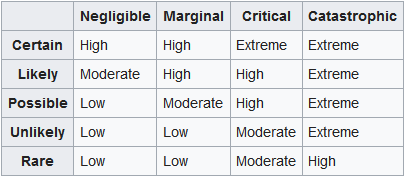
\includegraphics[width=.3\linewidth]{pics/riskmatrix} 
\end{center} 
\caption{Risk matrix showing levels of risk for given likelihood and harm severity.\\}
\label{riskmatrix}
\end{figure}

%----------------------------------------------------------------------------------------
%----------------------------------------------------------------------------------------
\section{Law and Regulations}
The MEGA65 products, the MEGAphone and the desktop version, will have to comply with the relevant laws and regulations of the countries in which they are sold in. These laws and regulations are specific to each country, but the general definition and intent of the laws and regulations is similar in lots of places around the world, at least in regard to electronic consumer products. This similarity in laws and regulations comes, in part, from international organisations and standards being adopted or used as a starting point for country specific standards. While the potential damage to a project is catastrophic as it could force a project to be abandoned in the most extreme cases, the uncertainty is fairly low as the laws and regulations are placed in the public domain before being enacted and should be unambiguous. Two cases of laws and regulations causing problems where identified during the case studies. The Raspberry Pi was delayed due to electronic interference testing and the Spectrum Vega was delayed due to age rating testing. While both of these examples are European specific, they similar nature of the laws and regulations of many market places make them relevant for a large portion of the world. \\

The MEGA65 project is rated as a marginal level of damage to the project from a law and regulation related risk. This is due to the projects ability to adapt to change quite well and it doesn't have a strict time or cost constraints. If a product was found to breach electronic interference laws for example, the MEGA65 team would be able to redesign and test the new product with only marginal delays in time and cost. The MEGA65 team is aware of this risk and of the most notable examples of these laws, such as electronic interference and age rating testing, but not of the specific laws of each market they are intending to operate in. The project has indicated that they are intending to carry out specific research into the laws and regulations of certain markets. Until this research has been conducted, the project has been rated at a likely level of probability of occurring.  \\

Likelihood - Likely   \\
Potential damage - Marginal \\
Risk - High \\


\subsection{Brexit-like events}
There are no foreseeable Brexit-like events that would be likely to affect the MEGA65 project. Brexit itself is unlikely to affect the MEGA65 project as the project is largely based in Australia, with the desktop version being made in Germany. The potential market for the MEGA65 in the United Kingdom is small and there will likely be some level of agreement with current laws and regulations within the United Kingdom to reduce to the disruption to the market during the transition out of the EU. The project has been rated as unlikely to experience this type of risk. The potential damage to the MEGA65 project was rated as marginal. \\

Likelihood - Unlikely \\
Potential damage - Marginal \\
Risk - Low \\


\section{Project Constraints}
The MEGA65 project is not bound to tight constraints on project cost. The desktop form factor may be subject to more tight constraints but overall the project was started as a hobby and continues in part as a learning tool for students at Flinders University. The funding model is also largely not dependant on selling the product to generate a profit. The MEGA65 project is then rated as a unlikely probability of occurring and a marginal risk. \\

Likelihood - Unlikely \\
Potential damage - Marginal \\
Risk - Low \\


\section{Crowd-funding}
The MEGA65 is considering using crowd-funding to raise funds but importantly they will wait until the design and component selection is complete before launching the campaign.

\subsection{Contract of sale}
The fact the the MEGA65 team are waiting until much later in the productisation process to launch the crowd-funding campaign greatly reduces the risks associated with it. The risk comes from forming a contract of sale between MEGA65 project and backers of the crowd-funding campaign and that contract not being fur filled. This could lead to legal proceedings against the MEGA65 project. The fact that the MEGA65 project won't do this until a much later stage in productisation means the chance that the MEGA65 project will fail to deliver the product is greatly reduced. This is due to the uncertainty factor being reduced as a lot of the design and component selection is done as such is not uncertain but certain. The MEGA65 project is rated as a an unlikely probability that it would cause a critical amount of damage to the project. \\

Likelihood - Unlikely \\
Potential damage - Critical \\
Risk - Moderate \\


\subsection{Currency}
If the MEGA65 team does decide to go the crowd-funding route they will need to decide on what currency to operate in. The risk here is the currency exchange rate drops after receiving the funds and now the actual purchasing power of the funds may be reduced. This risk is increased with time, the longer you hold onto the funds without spending them the more chance the exchange rate will fluctuate. As the MEGA65 team will wait until the product is much further along in the productisation process before crowd-funding this time period will be significantly reduced. There are also some currency which are more stable, in general, and research into these would also reduce the risk by allowing the MEGA65 team to use a stable currency to raise funds in. Another aspect to consider is the currency in which the majority of the funds will be spent i.e. if most of the parts and components are coming from USA companies then it may make sense to use the USD as the crowd-funding currency. The MEGA65 project is rated as unlikely to experience these risks and it would most likely produce a marginal level of damage if it did occur. \\

- identify the main currency in which purchase are to be made, 

Likelihood - Unlikely \\
Potential damage - Marginal \\
Risk - Low \\


\subsection{Failure to meet goal}
Due to the funding model of the MEGA65 project their is a lot more flexibility in the way the project moves forward after this event, if it did occur. The MEGA65 project has no strict criteria on cost or time to release and should only suffer a delay in time if it did not reach the predetermined campaign goal of a crowd-funding campaign. The MEGA65 project is rated as having a possible chance of this occurring, this depends heavily on the reception of the MEGA65 products to the public and how much publicity the campaign receives. The MEGA65 project is rated as likely to receive a negligible amount of damage from this event, should it occur. \\

Likelihood - Possible \\
Potential Damage - Negligible \\
Risk - Low \\


\section{Sourcing old components}
The MEGA65 project plans to use a 3.5" floppy disk drive as a component in the desktop version of the MEGA65. This is because the Commodore 65 prototype featured an internal 3.5" floppy disk drive. This use of old components brings increased risk due to the part not being in mass-production or common usage as such the availability of stock may be limited and the price may increase dramatically if the component is rare or becomes rare. The risk becomes even greater if the component is no longer in production and it needs to be manufactured for the project. This risk also increases with time as it is almost certain, given a long enough time period, that every component will become obsolete and thus expensive to purchase or produce. The MEGA65 is certain to be exposed to this risk. The project is rated as having a marginal amount of damage caused due to the 3.5" inch floppy still being in production and available to purchase. \\

Likelihood - Certain \\
Potential Damage - Marginal \\
Risk - High  \\

MEGA65 plans to use floppy drives, mention this in chapter 4 too!

- advise to pre purchase components 
- pre-purchasing components

700 floppy drives in warehouse in Germany

\section{Use of 3rd party intellectual property}
THE MEGA65 project has exposure to this risk in several areas. Due to the nature of the MEGA65 project and retro revival projects in general being inspired by products from the past, there is commonly intellectual property that the revival projects want to use or imitate to better replicate their inspiration. This is true for the MEGA65 project, being inspired by the Commodore 64 and 65, there are several areas in which being similar to these machine would greatly help the MEGA65 project. They are listed here:

\begin{enumerate}
\item Commodore logo on Commodore key
\item Commodore 64 software including games
\item Commodore 64 character set
\item Commodore 64 BASIC ROM
\item Commodore kernel ROM
\item Use of Commodore name
\end{enumerate}

\textbf{Commodore logo on Commodore key} \\
The Commodore 64 and 65 featured a special Commodore key with a commodore icon on it (sometimes referred to as "C="). The MEGA65 desktop form factor will need a key to function as the Commodore key if it to run Commodore 64 software. It would help users of the MEGA65 understand what the key is used for if the icon on it made users think of the Commodore key. An exact copy of the Commodore icon would fulfil this perfectly but it is a trademark, along with the Commodore name, as such they both carry risk in using. The MEGA65 project is certain to encounter this risk and there is a critical amount of potential damage that could be caused in using the Commodore icon. \\

Likelihood - Certain \\
Potential Damage - Critical \\
Risk - Extreme \\


\textbf{Commodore 64 software including games}\\
The software in question is specifically applications such as games, text editors or other a productivity software as some non-exhaustive examples, not the kernel or BASIC environment software. The MEGA65 aims to be compatible with as many Commodore 64 software titles as possible. This allows a more authentic experience for those seeking to recreate their Commodore 64 experiences. To achieve this the MEGA65 needs software to run on it and specifically it needs the software from the home computer era, created for the Commodore 64, to truly recreate the experience. This software is intellectual property as such its use without an agreement brings risks from legal action taken by the IP holders to protect their property. The MEGA65 project is planning on only including with their products, 3rd party software with which they have implicit agreement from the rights holders to use their intellectual property. This could either be from the rights holders stating their software is free to use to the public or through the MEGA65 team reaching out to the rights holders and them forming an agreement. Because of this the MEGAG65 project has been rated as having a rare likelihood of experiencing this event. The potential damage caused by this event comes in three parts: \\
a) The loss of user experiences and value to the user of the MEGA65 \\
b) The loss of time spent removing games from memory, documentation and promotional material \\
c) The loss of time and money responding to legal challenges and rulings \\
The MEGA65 project would be expected to experience negligible damage from a) and b). The damage from c) would be marginal as the MEGA65's market is likely to be small so any potential losses to rights holders would also be small which would suggest and legal ruling awarding the rights holders for loss of earnings would also be small. \\

Likelihood - Rare \\
Potential Damage - Marginal \\
Risk - Low \\

\textbf{Commodore 64 character set}\\
The MEGA65 requires a set of character bitmaps stored in memory, this is used to display text on the screen. The Commodore 64 character set would be ideal for this purpose as it is readily available from numerous website and would help the MEGA65 replicate the Commodore 64 more closely. The Commodore 64 character set is intellectual property, as such its use in the MEGA65 project brings risk. The MEGA65 project currently does not have an agreement to use the Commodore 64 character set. There is a certain likelihood of this occurring and a marginal level of damage that could occur. \\

Likelihood - Certain \\
Potential Damage - Marginal \\
Risk - High  \\


\textbf{Commodore 64 BASIC ROM}\\
The MEGA65 requires a BASIC ROM which will provide the BASIC environment into which it boots into on start up. This ROM, of which there are numerous versions specific to differing versions of BASIC, should be a ROM which provides the greatest amount of compatibility with Commodore 64 and 65 software, as the user will derive greater facility from it. The Commodore 64 BASIC ROM would be the ideal candidate but it is intellectual property and will attract risk if used. The MEGA65 project currently does not have an agreement to use the Commodore 64 BASIC ROM. The MEGA65 project is certain to experience this risk with the potential damage being critical. \\

Likelihood - Certain \\
Potential Damage - Critical \\
Risk - Extreme \\


\textbf{Commodore 64 kernel ROM}\\
The MEGA65 requires this ROM for basic functionality and it is of critical importance to the compatibility of the MEGA65 with Commodore 64 software that the kernel used function as the Commodore 64 kernel does. The ideal candidate kernel if only the functionality of the MEGA65 is considered, is the Commodore 64 kernel. This kernel is intellectual property as such it will attract a risk if used without an agreement with the rights holder. The MEGA65 project does not currently have an agreement with the rights holder. The potential damage from this risk is from the rights holder undertaking legal action against the MEGA65 project. The likelihood of this event occurring is considered unlikely as the ROM has been available online for decades with no noticeable attempt to control its distribution. The potential damage is catastrophic as the MEGA65 could not function without a kernel and if the Commodore 64 kernel was not able to be used suddenly, the MEGA65 would effectively be useless until a replacement was found. \\

Likelihood - Unlikely \\
Potential Damage - Catastrophic
Risk - Extreme


This is the main problem area:
- MEGA65 wanted to use a Commodore logo on the Commodore keyboard key
ask Paul if they had agreement to use commodore icon
recommend they don't use Commodore icon but a similar design

- MEGA65 NEEDS to use BASIC ROM/s to function as a Commodore compatibly computer
ask paul if they have agreement
recommend they don't use 3rd party BASIC ROM and consider producing their own

- games and applications licence

\section{Open-source business}
The MEGA65 project will be exposed to this risk, which is related to competitors being able to produce and sell the MEGA65 with no money being generated for the MEGA65 team. This means it can be harder to operate as a traditional electronics business in which its products are propriety and they can discourage competitors using there designs with legal challenges. The MEGA65 project is likely to not have a large market, as such the cost to enter the market is quite high compared to the potential profits. This will help reduce the likelihood of this occurring as long as the assumption that the MEGA65's market is small, remains true. The MEGA65 project is rated as possible for the likelihood of this occurring and a critical level of damage could be caused. \\

Likelihood - Possible \\
Potential Damage - Critical \\
Risk - High \\


\section{Loss of intellectual property}
This relates to the loss of agreement to use intellectual property that is require for the MEGA65. This occurred the most dramatically in the Vega Plus case study where the CTO left RCL and refused to let them use his prototype, which they had shown in their promotional videos. The MEGA65 is entirely shielded from this due to the open-source nature of the designs used throughout the entire project. No team member owns any part of the design as such they cannot withdraw their agreement for MEGA65 to use it. The MEGA65 project is rated as having a rare chance (the lowest) of occurring this event and of it doing negligible damage.  \\

Likelihood - Rare \\
Potential Damage - Negligible \\
Risk - Low \\


\section{Supplier failure}
The MEGA65 is exposed to this risk where ever they purchase from a 3rd party. The potential damage and likelihood of this event occurring is specific to each supplier and each purchase. The likelihood of this event occurring can be reduced by using reputable established suppliers as well as undertaking due diligence into suppliers before entering into agreements.



\section{Open-source fair use}
should not be a concern for MEGA65

ask paul if they used any open-source components


\section{Physical production problems}


\section{Advice on how to reduce MEGA65 project risk exposure}
In this section practical, actionable advice will be given on how to MEGA65 project can reduce their exposure to the risks identified in chapter \ref{Chapter4}. Using the risk evaluation of the MEGA65 project as of July 2018 as a starting point, this section aims to reduce the risk by focusing on the highest risk areas and suggesting strategies to reduce the risks.

 
%%Chapter 6 - Re-evaluating the MEGA65 project against known risks
% 	Did the MEGA65 project reduce its risk after 10 months?

\chapter{Risk evaluation of the MEGA65 project in May 2019}
\label{Chapter6}
After a 10 month period, the MEGA65 project was re-evaluated against the risks identified in Chapter \ref{Chapter3}. This period of time gave the project sufficient time to act on the suggestions given at the end of Chapter \ref{Chapter5}. By re-evaluating the MEGA65 project and comparing the result with the evaluation from July 2019, it is hoped that a conclusion can be drawn on whether the MEGA65 project reduced its risk exposure or not. 
%----------------------------------------------------------------------------------------
%----------------------------------------------------------------------------------------

\section{Laws and regulations}
The MEGA65 project has undertaken some research into the laws and regulation which need to be upheld in some of their key markets in which they expect to operate. With the knowledge gained from the research, the uncertainty in the relevant laws and regulations is reduced, as such the overall risk to the project is reduced. Not every market was researched, and the unknown markets still expose the project to risk if the MEGA65 where to be sold within it. The MEGA65 project is rated as having an unlikely chance of occurring and if it causing a marginal level of potential damage. \\

\begin{tabular}{l|l} % <-- Alignments: l=left, c=centre, r=right
    	\textbf{Category} 	&	\textbf{Rating} \\
      \hline
     Likelihood			&	Unlikely \\
     Possible Damage 	& 	Marginal \\
     Risk 				&	Low		\\	
    \end{tabular}


\section{Sourcing old components}
During the interim 10 months the MEGA65 project purchased 700 3.5" floppy disk drives and has them in storage in Germany. These disk drives are to be used as components during the assembly of the MEGA65 desktop version. This action of purchasing a large surplus of stock allows the MEGA65 project to avoid this risk in the medium term. When the stock runs out the risk will increase, as such the risk is largely tied to the MEGA65's popularity and sales volume. If the MEGA65 becomes hugely popular then this risk could increase dramatically. If the MEGA65 sells as expected by the MEGA65 project team, then 700 drives will be sufficient for the medium to long term. The potential damage the MEGA65 project is rated as marginal and the chance of it occurring possible. \\

\begin{tabular}{l|l} % <-- Alignments: l=left, c=centre, r=right
    	\textbf{Category} 	&	\textbf{Rating} \\
      \hline
     Likelihood			&	Possible \\
     Possible Damage 	& 	Marginal \\
     Risk 				&	Moderate		\\	
    \end{tabular}


\section{Use of 3rd party intellectual property}
The MEGA65 project has enacted some of the suggestions from Chapter \ref{Chapter5}. The steps undertaken in the identified risk areas are discussed below.

\subsection{Commodore logo}
The MEGA65 team decided to use their own design for the logo on the Commodore keyboard key. They have created and used the design for the pre-production run of the desktop form factor. This new design should completely remove the potential for this risk to effect the MEGA65 project.

\subsection{Commodore 64 character set}
The MEGA65 have decided to replace the Commodore character set with one they have created themselves from other freely available character sets and their own work. By removing the Commodore character set the risk is eliminated. 

\subsection{Commodore BASIC ROM and kernel ROM}
The MEGA65 team have decided to created their own BASIC and kernel ROMs. This reimplementation is currently under way and can provide basic functionality at this stage. By removing the Commodore ROMs from the MEGA65, the risk is entirely eliminated. \\

\begin{tabular}{l|l} % <-- Alignments: l=left, c=centre, r=right
    	\textbf{Category} 	&	\textbf{Rating} \\
      \hline
     Likelihood			&	Rare \\
     Possible Damage 	& 	Negligible \\
     Risk 				&	Low		\\	
    \end{tabular}


\section{Open-source business}
The MEGA65 team have not trademarked the MEGA65 name and are operating under the assumption that the MEGA65 will not be hugely popular. The MEGA65 team have been made aware of the strategies listed in Chapter \ref{Chapter5}, these strategies are only sensible if the MEGA65 becomes hugely popular and cannot be enacted to much benefit before. Because the MEGA65 team is aware of these strategies the MEGA65 project's potential damage and chance of occurring are both lowered compared to July 2018. \\

\begin{tabular}{l|l} % <-- Alignments: l=left, c=centre, r=right
    	\textbf{Category} 	&	\textbf{Rating} \\
      \hline
     Likelihood			&	Unlikely \\
     Possible Damage 	& 	Moderate \\
     Risk 				&	Low		\\	
    \end{tabular}



%%Chapter 7 - What is required to bring the MEGA65 to a MVP and market?
%What is required to bring the MEGA65 to a MVP and market?

\chapter{What is required to bring the MEGA65 to a MVP and market?}
\label{Chapter7}
This chapter discusses the possible features the MEGA65 should included to meet the expectations and needs of users. It looks at both form-factors of the MEGA65, the hand-held console and well as the desktop computer form-factor. After listing the features likely to be wanted by users and determining a MVP (Minimum Viable Product), this chapter discusses the work needed to be done to bring the MEGA65 to the stage of a MVP.

%----------------------------------------------------------------------------------------
%----------------------------------------------------------------------------------------

\section{Use cases}
This sections lists and discusses use cases for the MEGA65 in both its form-factors, the desktop computer and the hand-held console. By studying the way the MEGA65 might possibly be used and extracting the features required to fur fill each use case and then ranking them in order of importance, it is possible to create a list of features will be of high value to users of the MEGA65. This list can then help with decision making regarding the MVP of the MEGA65. The importance field is a rating of how important to the user the use case is likely to be from low, medium, high and critical. 

\textbf{Play Pre-installed Game Use Case} \\
\textbf{Importance} - high. \\
\textbf{Goal} - The user wants to play a game from the selection of games which are on the MEGA65, in either form-factor, on release. \\
\textbf{Story} - User turns on the MEGA65 and navigates to game selection menu, selects game and begins to play using the built-in controls. User wants to be able hear the game sounds and adjust sound volume. Once user is done, they wish to be able to quit the game and return to the MEGA65 menu system and have the ability select another game and play it. \\
\textbf{Features required} \begin{enumerate}
\item Functional and stable OS.
\item Pre-installed games on the MEGA65 with relevant licences obtained to use them.
\item Menu system to display installed games and to allow selection of a game.
\item Functional speaker and volume controls.
\item In-built controls are functional, responsive and ergonomic.
\item In-game menu system which allows user to quit the game and return to MEGA65 main screen. 
\item Case is ergonomic where it is to be held (hand-held version only).\\
\end{enumerate}


\textbf{Play Game Which is Stored on External Media Use Case} \\
\textbf{Importance} - high. \\
\textbf{Goal} - The user wants to play a game which currently resides on external media. \\
\textbf{Features required} \begin{enumerate}
\item Functional and stable OS.
\item External port to connect to users external media.
\item Menu system to display installed games and to allow selection of a game.
\item Functional speaker and volume controls.
\item In-built controls are functional, responsive and ergonomic.
\item In-game menu system which allows user to quit the game and return to MEGA65 main screen. 
\item Case is ergonomic where it is to be held (hand-held version only).\\
\end{enumerate}


\textbf{Attach and Use External Joystick Use Case}
\textbf{Actor} - A user who wants to use an external joystick to play games or control another program.
\textbf{Goal} - The user connects and is bale to use the an external joystick to interact with the MEGA65.




%


%----------------------------------------------------------------------------------------
%	THESIS CONTENT - APPENDICES
%----------------------------------------------------------------------------------------

\appendix % Cue to tell LaTeX that the following "chapters" are Appendices

% Include the appendices of the thesis as separate files from the Appendices folder
% Uncomment the lines as you write the Appendices

%\include{Appendices/AppendixA}
%\include{Appendices/AppendixB}
%\include{Appendices/AppendixC}

%----------------------------------------------------------------------------------------
%	BIBLIOGRAPHY
%----------------------------------------------------------------------------------------
%\bibliographystyle{ieeetr}
%\bibliography{reference_library}

% To have the biber command work uncomment the next line and comment out the other bibliography lines.
\printbibliography

%----------------------------------------------------------------------------------------

\end{document}  
